% Copyright (c) 2016, Mario Preishuber. All rights reserved.
%
% Notation: <option description> (<options>)
%
% Specify
%   - layout (onecolumn, twocolumn),
%   - thesis type (bachelor, master),
%   - language (english, naustrian)
%   - indicate that you want to use the university seal as background of the
%     titlepage (seal)
%   - indicate that you want signature fields (signatures)
%   - chapter headings to be on the next page or the next recto, verso page
%     (openany, openright, openleft) (standard memoir option, passed through)
\documentclass[onecolumn, openright, master, english, signatures]{dbrgrptt}
\usepackage[round-precision=2,round-mode=places,scientific-notation=engineering]{siunitx}
\usepackage[nameinlink]{cleveref}
\usepackage{listings}
\usepackage{multirow}
\usepackage{csvsimple}
\usepackage{rotating}
\usepackage[numbers]{natbib}
\usepackage{tikz}
\usetikzlibrary{arrows, fit, positioning, shapes}
\tikzset{%
  block node/.style={rectangle,draw,align=center, minimum width=1.5cm, minimum height=1.0cm},
  cpu node/.style={rectangle,draw,align=center, minimum width=1.5cm, minimum height=1.0cm, fill=black!30},
  cache node/.style={rectangle,draw,align=center, minimum width=1.5cm, minimum height=1.0cm, fill=green!30},
}

\definecolor{red}{RGB}{221,17,68}
\definecolor{orange}{RGB}{239,133,53}
\definecolor{yellow}{RGB}{255,202,40}
\definecolor{green}{RGB}{124,168,43}

\tikzstyle{cache-load}=[draw=green, line width=0.5mm, rectangle, rounded corners=0.5mm, minimum size=4mm, scale=0.7]
\tikzstyle{cache-store}=[fill=yellow, draw=yellow, line width=0.5mm, rectangle, rounded corners=0.5mm, minimum size=4mm, scale=0.7]
\tikzstyle{memory-load}=[draw=orange, line width=0.5mm, circle, scale=0.7]
\tikzstyle{memory-store}=[fill=red,draw=red, line width=0.5mm, circle, scale=0.7]


\hypersetup{
    colorlinks=false,
    pdfborder={0 0 0},
}

\begin{document}

%%%%%%%%%%%%%%%%%%%%%%%%%%%%%%%%%%%%%%%%%%%%%%%%%%%%%%%%%%%%%%%%%%%%%%%%%%%%%%%%
% Titling page / Initialization
%%%%%%%%%%%%%%%%%%%%%%%%%%%%%%%%%%%%%%%%%%%%%%%%%%%%%%%%%%%%%%%%%%%%%%%%%%%%%%%%

\thesistitle{%
Towards cache-optimal address allocation:%
% ~How fast could your code have run if you had known where to allocate memory?%
~How slow is your code?
}%
\thesisdate{\today}%
\thesisauthor{Mario Preishuber}{01120643}%
\setsupervisor{Univ.-Prof. Dr. Christoph Kirsch}%

% pages after this command (and before \mainmatter) are numbered roman
\frontmatter%

\hypersetup{pageanchor = false}%

%%%%%%%%%%%%%%%%%%%%%%%%%%%%%%%%%%%%%%%%
% titlepage / Titelseite
\maketitle%

%%%%%%%%%%%%%%%%%%%%%%%%%%%%%%%%%%%%%%%%
% statement of authentication / Verfassungserklaerung
\authenticationstatement%

%%%%%%%%%%%%%%%%%%%%%%%%%%%%%%%%%%%%%%%%
% acknowledgments / Danksagung
\acknowledgments{
Es ist an der Zeit einigen Begleitern auf meinem Weg dankzusagen.
\\~\\
% Christoph Kirsch
Ein großes Dankeschön gebührt meinem Betreuer \emph{Prof. Christoph Kirsch} für die Betreuung durch mein Bachelor- und Masterstudium. Du hast meine Entwicklung voran getrieben und mich stets zu Höchstleistungen motiviert; du hast mir Türen geöffnet von denen ich nicht zu träumen gewagt hätte; für diese wertvollen Erfahrungen möchte ich dir danken.
\\~\\
% Mama & Papa
Am Ende meines Studiums angekommen, möchte ich mich bei meiner \emph{Familie} bedanken. Insbesondere gilt der Dank meinen Eltern, Günther und Helga, für ihr Vertrauen und ihre Unterstützung. Danke, dass ihr mir dieses Studium ermöglicht habt.
\\~\\
% Alexander Miller
Dankeschön auch an \emph{Alexander Miller} für die wertvollen Diskussionen, welche dieses Projekt vorangetrieben haben.
\\~\\
% Thomas Hütter
Abschließend möchte ich mich noch bei \emph{Thomas Hütter} bedanken; für die unzähligen Stunden, die wir mit Projekten verbracht haben.
\\~\\
\textbf{Danke.}
}

%%%%%%%%%%%%%%%%%%%%%%%%%%%%%%%%%%%%%%%%
% abstract / Kurzfassung
\abstract{%
% motivation
The latency of accessing data stored in the main memory is a known problem in computer systems.
% problem statement
We are interested in finding metrics that characterize the performance of a program for a given cache.
% methods & approach
We analyze the characteristic of \emph{load} and \emph{store} instructions, called the \emph{memory access trace}, of two well known benchmark suites, namely SPEC 2006 and V8.
For our analysis about the potential performance improvement in terms of memory access performance and memory usage we modify the addresses used by a memory access trace.
% results & conclusion
Our analysis illustrates that for some benchmarks we are able to improve the memory usage and the memory access performance by a factor of at least two.
Nonetheless, the chosen metrics illustrate tendencies for improvement rather than unique characteristics.
}

%%%%%%%%%%%%%%%%%%%%%%%%%%%%%%%%%%%%%%%%
% table of contents / Inhaltsverzeichnis
\setcounter{tocdepth}{5}
\tableofcontents%

\hypersetup{pageanchor = true}%
%

%%%%%%%%%%%%%%%%%%%%%%%%%%%%%%%%%%%%%%%%%%%%%%%%%%%%%%%%%%%%%%%%%%%%%%%%%%%%%%%%%%%%%%%%%%%%%%%%%%%
% Main content
%%%%%%%%%%%%%%%%%%%%%%%%%%%%%%%%%%%%%%%%%%%%%%%%%%%%%%%%%%%%%%%%%%%%%%%%%%%%%%%%%%%%%%%%%%%%%%%%%%%

\mainmatter%

%%%%%%%%%%%%%%%%%%%%%%%%%%%%%%%%%%%%%%%%%%%%%%%%%%%%%%%%%%%%%%%%%%%%%%%%%%%%%%%%%%%%%%%%%%%%%%%%%%%
%%%%%%%%%%%%%%%%%%%%%%%%%%%%%%%%%%%%%%%%%%%%%%%%%%%%%%%%%%%%%%%%%%%%%%%%%%%%%%%%%%%%%%%%%%%%%%%%%%%
%%%%%%%%%%%%%%%%%%%%%%%%%%%%%%%%%%%%%%%%%%%%%%%%%%%%%%%%%%%%%%%%%%%%%%%%%%%%%%%%%%%%%%%%%%%%%%%%%%%
%%%%%%%%%%%%%%%%%%%%%%%%%%%%%%%%%%%%%%%%%%%%%%%%%%%%%%%%%%%%%%%%%%%%%%%%%%%%%%%%%%%%%%%%%%%%%%%%%%%
\chapter{Introduction}\label{cha:introduction}
% motivation
Caches are based on two major observations: Data that is accessed once is likely (1) that nearby data is accessed in near future (\emph{spatial locality}~\cite{jacob2010memory}) and (2) that the same data is accessed again in near future (\emph{temporal locality}~\cite{jacob2010memory}).
To address spatial locality so-called \emph{cache lines} have been introduced.
A cache line is the smallest unit of data that can be loaded from the main memory.
All cache lines of a cache are of the same size and dependent on the cache line size the values of multiple addresses fit in one cache line.
A program accesses the data stored in the main memory via \emph{addresses}.
An address is a unique identifier for a certain amount of data, e.g. 8 byte are a common amount of data accessible by one address~\cite{patterson2011computer}.
%
There are two different types of memory accesses, reading and modifying.
Reading data is realized by executing a \emph{load} instruction.
A load instruction reads the data of an address and stores the read value into one of the \ac{CPU}s registers for further computations.
The process of reading the data first tries to read the data from cache.
If the data of the requested address is in the cache it is read from there.
Otherwise the data has to be read from the main memory.
Data is loaded from the main memory, stored in the cache, and finally loaded into one of the \ac{CPU}s registers.
To modify data, a \emph{store} instruction has to be executed.
If the data to modify is already in the cache the main memory is not accessed.
Otherwise, the data has to be loaded from the main memory into the cache first.
Independent of the access type, if the accessed data is available in the cache this is called a \emph{cache hit}, otherwise when the data is not in the cache this is called a \emph{cache miss}.
%
Since, a cache is limited in space and typically the data required for the execution, which is called the \emph{working set}~\cite{denning1968working}, is larger then the cache size, eventually the cache will run out of space.
Whenever the cache is full and an address is accessed that is not in the cache it is required to free up space.
For this reason every cache implements an \emph{eviction policy} to decide on an eviction candidate.
The eviction candidate is written back to the main memory to make space for the requested data, it is \emph{evicted}.
The choice of the eviction policy aims to satisfy temporal locality, e.g. a common eviction policy is to evict the least recently used address.
%
The fact that data is grouped together is so-called \emph{cache lines} influences the cache performance significantly.
Assume iterating over an array.
In such a case the performance might be excellent, because these are perfect conditions for spatial locality and temporal locality.
However, assume iterating over a dynamically allocated linked list.
Compared to an array it is not ensured that the list elements are stored contiguous in memory.
It is more likely that elements are distributed across the whole address space.
In a worst case scenario each iteration forces a cache miss.
This issue is a consequence of the \emph{memory layout} generated by the allocator through dynamic allocations.

% problem statement
We are interested in the following problem: given a trace of load and store instructions, can we find metrics that characterize the trace performance for a given cache and implement an execution engine for computing their quantities?

% methods & approach
For the purpose of this work we focus on the sequence of load and store instructions of a program, the so-called \emph{memory access trace} (short \emph{trace}).
We analyze traces of the SPEC 2006 benchmarks and the V8 benchmarks.
For each trace of a benchmark the following four metrics are computed:
(1) the \emph{accesses} represents the number of accesses on an address,
(2) the \emph{access distance} is defined as the number of accesses on other addresses between to accesses on the same address,
(3) the \emph{liveness interval length} represents the timespan an address is in use, and
(4) the \emph{overlapping liveness} is defined as the number of overlapping liveness intervals at a certain point of the execution.
In this work each store instruction indicates the beginning of a liveness interval.
A liveness interval ends with the last load instruction before the next store instruction, i.e. an address might consist of multiple liveness intervals.
%
First, our analysis observe the sequence of load and store instructions of a benchmark.
Next, the observed trace is analyzed according to the four metrics, \emph{accesses}, \emph{access distance}, \emph{liveness interval length}, and \emph{overlapping liveness}.
After the metrics have been saved the procedure for the performance analysis starts.
The performance analysis uses different \emph{allocators} to modify the addresses used by the trace.
The modification of the used addresses is called \emph{trace transformation}.
Each transformed trace is executed on four simulated caches.
The simulated caches differs in the applied eviction policy and their information about the executed trace.
During the execution, the number of main memory accesses, the number of cache misses, and cache hits are counted to determine the performance of a trace for a certain simulated cache.

% conjecture
Our conjecture is that the four metrics \emph{accesses}, \emph{access distance}, \emph{liveness interval length}, and \emph{Overlapping Liveness} characterize the performance of a program.
Furthermore, we are convinced that caches may be more effective if memory is reused quickly and independently of where the data is located.


%%%%%%%%%%%%%%%%%%%%%%%%%%%%%%%%%%%%%%%%%%%%%%%%%%%%%%%%%%%%%%%%%%%%%%%%%%%%%%%%%%%%%%%%%%%%%%%%%%%
%%%%%%%%%%%%%%%%%%%%%%%%%%%%%%%%%%%%%%%%%%%%%%%%%%%%%%%%%%%%%%%%%%%%%%%%%%%%%%%%%%%%%%%%%%%%%%%%%%%
%%%%%%%%%%%%%%%%%%%%%%%%%%%%%%%%%%%%%%%%%%%%%%%%%%%%%%%%%%%%%%%%%%%%%%%%%%%%%%%%%%%%%%%%%%%%%%%%%%%
%%%%%%%%%%%%%%%%%%%%%%%%%%%%%%%%%%%%%%%%%%%%%%%%%%%%%%%%%%%%%%%%%%%%%%%%%%%%%%%%%%%%%%%%%%%%%%%%%%%

\chapter{Theoretical Foundations}\label{cha:theoretical-foundations}

%%%%%%%%%%%%%%%%%%%%%%%%%%%%%%%%%%%%%%%%%%%%%%%%%%%%%%%%%%%%%%%%%%%%%%%%%%%%%%%%%%%%%%%%%%%%%%%%%%%
% Hardware Model
%%%%%%%%%%%%%%%%%%%%%%%%%%%%%%%%%%%%%%%%%%%%%%%%%%%%%%%%%%%%%%%%%%%%%%%%%%%%%%%%%%%%%%%%%%%%%%%%%%%

\section{Hardware Model}\label{sec:hardware-model}

This section deals with the applied hardware model. The model used is reduced to the minimal required core components of a modern computer system. It consists of three components as illustrated in \Cref{fig:hardware-model}. The three components are the central processing unit, a cache, and the main memory.

\begin{figure}[!ht]
  \centering
  % +-----+ store  +---------+ store  +-------------+
% |     |------->|         |------->|             |
% | CPU |        |  Cache  |        | Main Memory |
% |     |<-------|         |<-------|             |
% +-----+  load  +---------+  load  +-------------+
\begin{tikzpicture}
% CPU
\node (cpu)[stdnode, minimum width=2cm, minimum height=2cm] at (1,1) {CPU};
% Cache
\node (cache)[stdnode, minimum width=2cm, minimum height=2cm] at (5,1) {Cache};
% Main Memory
\node (memory)[stdnode, minimum width=4cm, minimum height=2cm] at (10,1) {Main Memory};


% Communication between CPU and Cache
\draw [arrow] (2,1.5) -- (4,1.5);
\node [above,align=center] at (3,1.5) {Cache\\Store};
\draw [arrow] (4,0.5) -- (2,0.5);
\node [below,align=center] at (3,0.5) {Cache\\Load};

% Communication between Cache and Main Memory
\draw [arrow] (6,1.5) -- (8,1.5);
\node [above,align=center] at (7,1.5) {Memory\\Store};
\draw [arrow] (8,0.5) -- (6,0.5);
\node [below,align=center] at (7,0.5) {Memory\\Load};

\end{tikzpicture}

  \caption{Hardware Model}
  \label{fig:hardware-model}
\end{figure}

\subsection{Central Processing Unit}
The \emph{\ac{CPU}} is the heart of a computer system. The purpose of a \ac{CPU} is to process and execute a given program. A \emph{program} consists of a sequence of instructions which operate on data. It is processed sequentially, that is, instruction by instruction. An \emph{instruction} is a command with the purpose to perform a specific action, e.g. to add two numbers or to modify data. \emph{Data} is the information required by a program that is necessary for its execution, e.g. values for computations. The \ac{CPU} consists of a limited number of so-called \emph{registers}. A \emph{register} is an extremely small and extremely fast memory unit which allows the \ac{CPU} to execute computations. Registers are the only memory unit where the \ac{CPU} is able to apply arithmetic operations. The actual size of a single register and the number of registers available for computations depend on the architecture of the hardware.

For the purpose of this work, only instructions reading or writing data are taken into account. In order to read data, a \emph{load} instruction is required; in order to write data, a \emph{store} instructions is applied. These two instructions access the data of a program stored at the main memory, e.g. for the purpose of a calculation it might be necessary to get some data from the main memory and save its result at the main memory for later usage. Such data can be accessed by executing a load or store instruction on main memory. However, there are several more instructions available on modern computer systems, e.g. arithmetical operations.

\subsection{Main Memory}
The \emph{main memory} is a storage containing all data required to execute a program. In general, the \ac{CPU} has to load data from the main memory and store data in main memory to process a program. Furthermore, even the program itself is stored at the main memory during its execution. Each instruction of a program has to be loaded before the \ac{CPU} is able to execute it. In case of a load instruction, the \ac{CPU} first loads the instruction itself. Then the CPU interprets the instruction to find out what to do, e.g. execute a load of data. Last the \ac{CPU} execution the instruction, e.g. it loads the actually required data into some of the available registers.

The main memory is structured in equally sized chunks of memory, that are for example the size of 8 byte. These are then called a \emph{word}. Each of these memory chunks can be accesses by the \ac{CPU} via a unique identifier, its \emph{physical address}. To simplify a programmers life and make programs easier portable, \emph{virtual addresses} have been introduced. A virtual address (short \emph{address}) maps a physical address. Each program on a computer is given its own virtual address space which starts at address 0; this is an important assumption. In reality the first physical address of a program is very unlikely to be 0. This mapping of physical addresses to virtual addresses which always start at address 0 makes programs easier portable. For the purpose of this work, it is important to keep in mind that load and store instruction operate on addresses, e.g. \texttt{load \&address} where \texttt{\&address} represents the address of the data that is to be loaded.

\subsection{Cache}
A \emph{cache} is a small high-speed memory which temporarily holds data of the addresses used by the currently processed program. The concept of caches has been introduced by Smith \cite{smith1982cache}.

Caches are based on two major observations, namely \emph{Temporal locality} and \emph{Spatial locality}.\emph{Temporal locality} means that if data is accessed it is likely that the same data is accessed again in the near future. \emph{Spatial locality} means that if data is accessed it is likely that other data near by is also accessed in the near future. Speaking about \emph{accessing an address} is equivalent with \emph{accessing data stored at an address in the main memory}. The same accounts for cached addresses. For the \ac{CPU} a cache is invisible. Regardless of whether or there is a cache or not the \ac{CPU} always just wants to access a certain address. If there is cache present it simply takes less time to load the value of an address into the \ac{CPU}s register. This is because caches are high-speed memory units.

A \emph{cache hit} occurs whenever the \ac{CPU} wants to access an address which is already in the cache. Then no main memory access is required. The data is directly accessed via cache.

A \emph{cache miss} occurs whenever the \ac{CPU} wants to access an address that is not currently in the cache. Such a situation requires to load the data of the requested address from the main memory into the cache. Before the value stored at this address is loaded into one of the registers. Such an operation is expensive as explained in \Cref{sec:performance}.

The \emph{cache policy} decides which address has to be \emph{evicted}, i.e., which address has to be written back into the main memory in order to make free space available. Since caches are limited in the number of addresses that can be temporarily, stored a cache will eventually run out of space. In case the cache is full and a cache miss occurs it is required to make space available to load the requested address. There are different algorithms trying to make an appropriate chose of the address that is to be evicted. For more details see \Cref{sec:caches}

%%%%%%%%%%%%%%%%%%%%%%%%%%%%%%%%%%%%%%%%%%%%%%%%%%%%%%%%%%%%%%%%%%%%%%%%%%%%%%%%%%%%%%%%%%%%%%%%%%%
% Memory Access Trace
%%%%%%%%%%%%%%%%%%%%%%%%%%%%%%%%%%%%%%%%%%%%%%%%%%%%%%%%%%%%%%%%%%%%%%%%%%%%%%%%%%%%%%%%%%%%%%%%%%%

\section{Memory Access Trace}\label{sec:memory-access-trace}

The \emph{\ac{trace}} represents all memory accesses for a given program. More precisely, the \ac{trace} is a sequence of load and store instructions observed by analyzing a given program. Furthermore, for the purpose of this work is does not matter which value is stored at a certain address. Therefore, the stored values are all dropped. This results in a sequence of tuples consisting of the instruction type, which is either \emph{load} or \emph{store}, and an address. \Cref{fig:mat-example-trace} shows an example of a \ac{trace}, addresses are annotated with \texttt{\&} known from programming languages like C.

\Cref{fig:mat-example-c-code} shows a simple C program which sums up three numbers. First, all used variables are declared. Afterwards, the variables \texttt{sum}, \texttt{x}, and \texttt{y} are initialized with the values \texttt{0}, \texttt{1}, and \texttt{2}. Followed by the first computation, the value of \texttt{x} is added to \texttt{sum}s value and stored in \texttt{sum}. Next, the variable \texttt{z} is initialized with value \texttt{3}. Then, \texttt{sum} is increased by the value of \texttt{y}. Finally, the computation is completed by adding the value of \texttt{z} to \texttt{sum}.

\begin{figure}[!ht]
  \centering
  \begin{tabular}{c}
  \lstinputlisting[language=C]{figs/code/memory-access-trace/mat.c}
  \end{tabular}
  \caption{C code example of summing three numbers.}
  \label{fig:mat-example-c-code}
\end{figure}

\Cref{fig:mat-example-assembly-code} shows a snippet of assembly code generated by compiling the code of \Cref{fig:mat-example-c-code}. For compilation GCC 4.8.5 on Ubuntu 16.04 for AMD Opteron\texttrademark Processor 6376 with x86\_64 Architecture has been used. Since the declaration of the variables is only important for the compiler, no assembly code is generated for: \texttt{int sum, x, y, z;}. Therefore, the first line of assembly code shown in \Cref{fig:mat-example-assembly-code} represents the code generated for the C code \texttt{sum = 0;}. However, the compiler has not generated a store operation, instead the following code appears \texttt{movl \$0, -16(\%rbp)}.

This assembly instruction consists of three parts. The first part shows the instruction that should be executed. In the example above \texttt{movl} represents this instruction. \texttt{movl} moves a \emph{long} value into a register. A long value is on the x86\_64 architecture the size of 32 bit. The second part represents the value that should be moved. In the example from above a constant value is moved. The fact that \texttt{0} is a constant value is indicated by the \texttt{\$} character. The third part represents the address to which the value should be moved to. In the example from above the target address is \texttt{-16(\%rbp)}. In this case, \texttt{rbp} is a register indicated by the \texttt{\%} character. Further, \texttt{\%rbp} is a so-called \emph{general-purpose} register of size 64 bit. By now it is enough to know that this register holds a memory address which is used as base to compute the actual target address. \texttt{-16} is the offset used to compute the actual target address.
\Cref{fig:mat-example-assembly-code} only consists of two different types of instructions. The \texttt{movl} instruction is explained above. The other operation is used as follows \texttt{addl \%eax -16(\%rbp)}. The meaning of this instruction is to add the value stored at \texttt{-16(\%rbp)} to the value currently stored at the register \texttt{\%eax} and store the result at \texttt{\%eax}. As indicated by the \texttt{l} character at the and of the instruction name, this instruction operates on values of size 32 bit.

\begin{figure}[!ht]
  \centering
  \begin{tabular}{c}
  \lstinputlisting[firstline=13, lastline=22]{figs/code/memory-access-trace/mat.s}
  \end{tabular}
  \caption{Assembly code snippet generated by compiling the code of \Cref{fig:mat-example-c-code} with GCC 4.8.5 on Ubuntu 16.04.5 for AMD Opteron\texttrademark~Processor 6376 with x86\_64 Architecture.}
  \label{fig:mat-example-assembly-code}
\end{figure}

Comparing the assembly code of \Cref{fig:mat-example-assembly-code} with the C code of \Cref{fig:mat-example-c-code}, the correlating instruction can be identified.
Obviously, the first three assembly instructions correlate to the three assignments of the C code.
It might be unexpected that the \texttt{movl} instruction is used instead of a store instruction.
However, moving a value to a certain location is semantically equivalent to a store.
Nevertheless, there are three addresses used, each with an offset.
These offsets increase exactly by the same size: four (-16, -12, and -8).
The operation \texttt{movl} operates on 32 bit which are 4 byte.
Hence, the variables \texttt{sum}, \texttt{x}, and \texttt{y} are stored contiguously in memory.

\begin{figure}[!ht]
  \centering
  \begin{tabular}{c}
  \begin{lstlisting}
sum = 0; | movl $0, -16(%rbp)
  x = 1; | movl $1, -12(%rbp)
  y = 2; | movl $2, -8(%rbp)
  \end{lstlisting}
  \end{tabular}
  \caption{Assignments: C code (left) and generated assembly code (right).}
  \label{fig:mat-example-comp-assignment}
\end{figure}

Different to assignments an addition leads to two lines of assembly code as illustrated by \Cref{fig:mat-example-comp-addition}.
The first instruction loads the value of \texttt{x} (stored at address \texttt{-12(\%rbp)}) into register \texttt{\%eax}.
Since the \ac{CPU} can apply arithmetic operations exclusively on registers, it is required to load the value of \texttt{x} into a register before computing the sum.
Again the \texttt{movl} instruction is used to load the data.
As before, the semantics of the \texttt{movl} is equivalent to a load instruction.
The second instruction generated is the actual computation.
The generated \texttt{addl} instruction operates on 32 bit, as well as the \texttt{movl} instruction.
Indicated by the last letter of the instruction name, \texttt{l}.
\texttt{addl} takes the value store in the register \texttt{\%eax} and adds the value store at the address \texttt{-16(\%rbp)}.
The result of this computation is stored in the \texttt{\%eax} register.

\begin{figure}[!ht]
  \centering
  \begin{tabular}{c}
  \begin{lstlisting}
sum = sum + x; | movl -12(%rbp), %eax
               | addl %eax, -16(%rbp)
  \end{lstlisting}
  \end{tabular}
  \caption{Addition: C code (left) and generated assembly code (right).}
  \label{fig:mat-example-comp-addition}
\end{figure}

After the addition, the assignment of variable \texttt{z} follows.
This assignment works exactly the same as discussed at the beginning of this section.
The same accounts for the remaining two additions (\texttt{sum = sum + y;} and \texttt{sum = sum + z;}).
The explanations above illustrate the generate code for the simple example of \Cref{fig:mat-example-c-code}.
Furthermore, the behavior of the code is discussed.
Moreover, there are already tiny hints about the memory accesses.
The next step is to take look at the \ac{trace} used in this work.

\Cref{fig:mat-example-trace} presents the \ac{trace} observed by the example of \Cref{fig:mat-example-c-code}.
For reasons of better human readability the variable names of the C code are kept.
To illustrate that the \ac{trace} operates on the addresses the C like character \texttt{\&} is used as prefix of an address.
All information expect the kind of access and the accessed address is dropped.

\begin{figure}[!ht]
  \centering
  \begin{tabular}{c}
  \lstinputlisting{figs/code/memory-access-trace/mat.trace.manual}
  \end{tabular}
  \caption{Memory access trace of the assembly code shown in \Cref{fig:mat-example-assembly-code}.}
  \label{fig:mat-example-trace}
\end{figure}

\Cref{fig:mat-example-comp-assignment-all} compares the assignment of the C code with the generated assembly code and the resulting \ac{trace} of these instructions.
Assignments are straight translated into stores within in the \ac{trace}.
In order to facilitate the procedure, the stored value is dropped so that only the accessed address remains in the \ac{trace}.

\begin{figure}[!ht]
  \centering
  \begin{tabular}{c}
  \begin{lstlisting}
sum = 0; | movl $0, -16(%rbp) | store &sum
  x = 1; | movl $1, -12(%rbp) | store &x
  y = 2; | movl $2, -8(%rbp)  | store &y
  \end{lstlisting}
  \end{tabular}
  \caption{Assignments: C code (left), generated assembly code (middle), and \ac{trace} (right).}
  \label{fig:mat-example-comp-assignment-all}
\end{figure}

\Cref{fig:mat-example-comp-addition-all} presents the \ac{trace} for the addition \texttt{sum = sum + x;}. The move instruction \texttt{movl -12(\%rbp), \%eax} loads the value of \texttt{x} into a register, which translates as expected into a load instruction in the \ac{trace}.
The addition itself translates into two instructions within the \ac{trace}.

\begin{figure}[!ht]
  \centering
  \begin{tabular}{c}
  \begin{lstlisting}
sum = sum + x; | movl -12(%rbp), %eax | load  &x
               | addl %eax, -16(%rbp) | load  &sum
                                      | store &sum
  \end{lstlisting}
  \end{tabular}
  \caption{Addition: C code (left), generated assembly code (middle), and \ac{trace} (right).}
  \label{fig:mat-example-comp-addition-all}
\end{figure}

An striking observation is that there are no arithmetic operations in the \ac{trace}, which makes sense, since this representation of a program shows all the interaction with the main memory.
However, this does not mean that while translating the assembly code to its \ac{trace} arithmetic operations could be skipped.
Nevertheless, not only the move instructions could lead to a main memory access.
\Cref{fig:mat-example-addition-detail} shows a main memory access that is achieved via reading the value stored at address \texttt{-16(\%rbp)} for the computation.
Such an instruction leads to a \texttt{load} within the \ac{trace}.
Since the result of a computation is saved somewhere there is also a \texttt{store} observable in \ac{trace}.

\begin{figure}[!ht]
  \centering
  \begin{tabular}{c}
  \begin{lstlisting}
addl %eax, -16(%rbp)
  \end{lstlisting}
  \end{tabular}
  \caption{Addition assembly code.}
  \label{fig:mat-example-addition-detail}
\end{figure}

This section showed how the \ac{trace} of a program is observed.
Hence, the assembly code of a simple C program which sums three numbers is discussed and finally the correlating \ac{trace} is presented.
The \ac{trace} of a program is a sequence of tuples.
Each of them holds the type of access which is either load or store and the accessed address.
An address is prefixed with an \texttt{\&}.

%%%%%%%%%%%%%%%%%%%%%%%%%%%%%%%%%%%%%%%%%%%%%%%%%%%%%%%%%%%%%%%%%%%%%%%%%%%%%%%%%%%%%%%%%%%%%%%%%%%
% Liveness
%%%%%%%%%%%%%%%%%%%%%%%%%%%%%%%%%%%%%%%%%%%%%%%%%%%%%%%%%%%%%%%%%%%%%%%%%%%%%%%%%%%%%%%%%%%%%%%%%%%

\section{Liveness}\label{sec:liveness}

This section introduces the concept of \emph{liveness of an address}.
Roughly speaking, the liveness of an address describes the timespan in which the address is used by a program.
In general, the liveness of an address begins with its allocation and ends with its deallocation as illustrated by \Cref{fig:liveness-classical}.
Yet, \citeauthor{aigner2013acdc} showed in their work \cite{aigner2013acdc} that the general understanding of liveness offers potential for improvement.

In their work, they introduced the term of \emph{deallocation delay}, describing the timespan from the last access on an object until its deallocation.
This is based on the observation that objects often live longer than necessary, because of this deallocation delay, which is a waste of resources, especially, memory.

\begin{remark}
Note that in the work \cite{aigner2013acdc} the liveness term is defined at object level. In this work we are exclusively focusing on address level.
\end{remark}

However, in this work liveness is defined differently.
First of all, liveness is defined on address level, since the whole work is operating on addresses rather than objects or data structures.
Further, an address does not consist of \emph{the one} liveness.
Rather, it consists of multiple timespans of liveness.
In the timespan beginning with allocating an address and deallocating it there are periods in which the address is used heavily and there are periods where the address is not used at all.
These periods of usage are called \emph{liveness intervals}.
How these liveness intervals are defined is presented by \Cref{def:liveness-interval}.
The basic idea is that each store operation introduces a new liveness intervals.
This is similar to the initialization of an address.

\begin{definition}[Liveness interval]\label{def:liveness-interval}
Whenever there is a store on an address a new \emph{liveness interval} begins. A liveness interval ends with the last access at the address before the next store instruction occurs. A liveness interval also ends with the absolute last access on the address.
\end{definition}

\begin{remark}
As an implication of Definition~\ref{def:liveness-interval} a single address might have multiple liveness intervals.
\Cref{fig:liveness-intervals-example} presents the liveness interval for the address of variable \texttt{sum}.
\end{remark}

\begin{figure}[!ht]
  \centering
  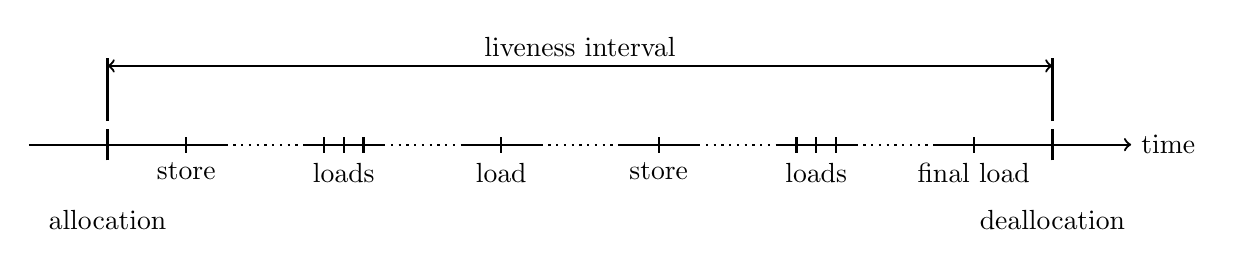
\begin{tikzpicture}
% The timeline
\draw [-][thick] (-1,0) -- (1.5,0);
\draw [dotted][thick] (1.5,0) -- (2.5,0);
\draw [-][thick] (2.5,0) -- (3.5,0);
\draw [dotted][thick] (3.5,0) -- (4.5,0);
\draw [-][thick] (4.5,0) -- (5.5,0);

\draw [dotted][thick] (5.5,0) -- (6.5,0);

\draw [-][thick] (6.5,0) -- (7.5,0);
\draw [dotted][thick] (7.5,0) -- (8.5,0);
\draw [-][thick] (8.5,0) -- (9.5,0);
\draw [dotted][thick] (9.5,0) -- (10.5,0);
\draw [->][thick] (10.5,0) -- (13,0) node[right]{time};

% Access ticks
\draw [-][thick] (0,-0.2) node[below=0.5]{allocation} -- (0,0.2);

\draw [-][thick] (1,-0.1) node[below]{store} -- (1,0.1);
\draw [-][thick] (3,-0.1) node[below]{loads} -- (3,0.1);
\draw [-][thick] (5,-0.1) node[below]{load} -- (5,0.1);
\draw [-][thick] (2.75,-0.1) -- (2.75,0.1);
\draw [-][thick] (3.25,-0.1) -- (3.25,0.1);

\draw [-][thick] (7,-0.1) node[below]{store} -- (7,0.1);
\draw [-][thick] (9,-0.1) node[below]{loads} -- (9,0.1);
\draw [-][thick] (11,-0.1) node[below]{final load} -- (11,0.1);
\draw [-][thick] (8.75,-0.1) -- (8.75,0.1);
\draw [-][thick] (9.25,-0.1) -- (9.25,0.1);

\draw [-][thick] (12,-0.2) node[below=0.5]{deallocation} -- (12,0.2);

% Liveness interval 1
\draw [-][thick] (0, 0.3) -- (0,1.1);
\draw [<->][thick] (0,1) -- (12,1);
\draw [-][thick] (12, 0.3) -- (12,1.1);
\node [above] at (6,1) {liveness interval};

\end{tikzpicture}

  \caption{Classical liveness}
  \label{fig:liveness-classical}
\end{figure}

\begin{figure}[!ht]
  \centering
  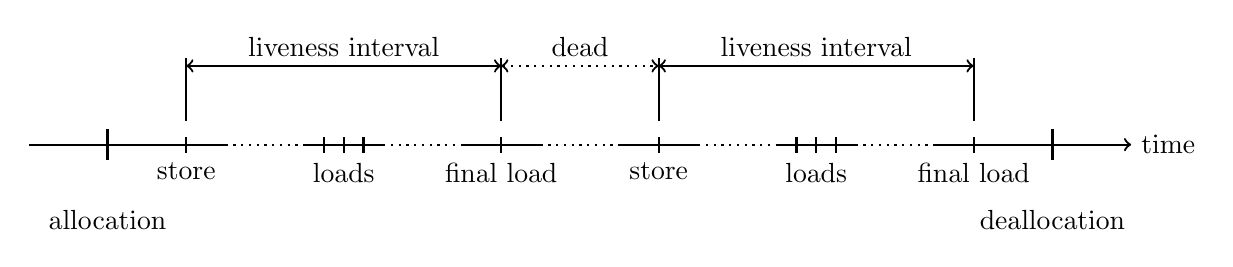
\begin{tikzpicture}
% The timeline
\draw [-][thick] (-1,0) -- (1.5,0);
\draw [dotted][thick] (1.5,0) -- (2.5,0);
\draw [-][thick] (2.5,0) -- (3.5,0);
\draw [dotted][thick] (3.5,0) -- (4.5,0);
\draw [-][thick] (4.5,0) -- (5.5,0);

\draw [dotted][thick] (5.5,0) -- (6.5,0);

\draw [-][thick] (6.5,0) -- (7.5,0);
\draw [dotted][thick] (7.5,0) -- (8.5,0);
\draw [-][thick] (8.5,0) -- (9.5,0);
\draw [dotted][thick] (9.5,0) -- (10.5,0);
\draw [->][thick] (10.5,0) -- (13,0) node[right]{time};

% Access ticks
\draw [-][thick] (0,-0.2) node[below=0.5]{allocation} -- (0,0.2);

\draw [-][thick] (1,-0.1) node[below]{store} -- (1,0.1);
\draw [-][thick] (3,-0.1) node[below]{loads} -- (3,0.1);
\draw [-][thick] (5,-0.1) node[below]{final load} -- (5,0.1);
\draw [-][thick] (2.75,-0.1) -- (2.75,0.1);
\draw [-][thick] (3.25,-0.1) -- (3.25,0.1);

\draw [-][thick] (7,-0.1) node[below]{store} -- (7,0.1);
\draw [-][thick] (9,-0.1) node[below]{loads} -- (9,0.1);
\draw [-][thick] (11,-0.1) node[below]{final load} -- (11,0.1);
\draw [-][thick] (8.75,-0.1) -- (8.75,0.1);
\draw [-][thick] (9.25,-0.1) -- (9.25,0.1);

\draw [-][thick] (12,-0.2) node[below=0.5]{deallocation} -- (12,0.2);

% Liveness interval 1
\draw [-][thick] (1, 0.3) -- (1,1.1);
\draw [<->][thick] (1,1) -- (5,1);
\draw [-][thick] (5, 0.3) -- (5,1.1);
\node [above] at (3,1) {liveness interval};

% Dead interval
\draw [-][thick] (5, 0.3) -- (5,1.1);
\draw [<->][thick, dotted] (5,1) -- (7,1);
\draw [-][thick] (7, 0.3) -- (7,1.1);
\node [above] at (6,1) {dead};

% Liveness interval 2
\draw [-][thick] (7, 0.3) -- (7,1.1);
\draw [<->][thick] (7,1) -- (11,1);
\draw [-][thick] (11, 0.3) -- (11,1.1);
\node [above] at (9,1) {liveness interval};

\end{tikzpicture}

  \caption{Liveness intervals}
  \label{fig:liveness-intervals}
\end{figure}

\Cref{fig:liveness-intervals-example} illustrates the liveness intervals of the C code example presented in \Cref{fig:mat-example-c-code}, which shows the instruction number on the left side and the instruction itself on the right side.
On top of the figure the addresses used by the program are listed.
The core of the figure illustrates the liveness intervals of the addresses.
Each line represents a single liveness interval.
A liveness interval begins at the lower instruction number and ends at the higher one.
The liveness intervals are quite obvious for the addresses \texttt{\&x}, \texttt{\&y}, and \texttt{\&z}.
According to Definition \ref{def:liveness-interval}, a liveness interval always begins with a store instruction.
The instructions 2, 3, and 7 indicate the beginnings of the liveness intervals for the three addresses \texttt{\&x}, \texttt{\&y}, and \texttt{\&z}.
The endings are indicated by load instructions at the instruction numbers 5, 9, and 12.
None of the addresses is accessed after these lines again, e.g. \texttt{\&x}, not used anymore after instruction number 5.
The address \texttt{\&sum} presents a much more interesting case, it consists of four liveness intervals.
The first liveness interval of \texttt{\&sum} begins at instruction number 1.
This is when \texttt{\&sum} is initialized.
Followed by the initializations of \texttt{\&x} and \texttt{\&y} before \texttt{\&sum} is accessed again.
The load at instruction number 4 indicates the end of \texttt{\&sum}s first liveness interval, because the next access is a store.
At instruction number 6 the second liveness interval begins.
The other liveness intervals follow the same pattern.
Note that also the store at instruction number 13 yields a liveness interval, even if it is the shortest possible.
At the instruction numbers 5, 9, and 12 the address \texttt{\&sum} is \emph{dead} according to the applied definition of liveness intervals, see \Cref{fig:liveness-intervals}.
It would allow to reuse the address of \texttt{\&sum} for other purposes.

\begin{figure}[!ht]
  \centering
  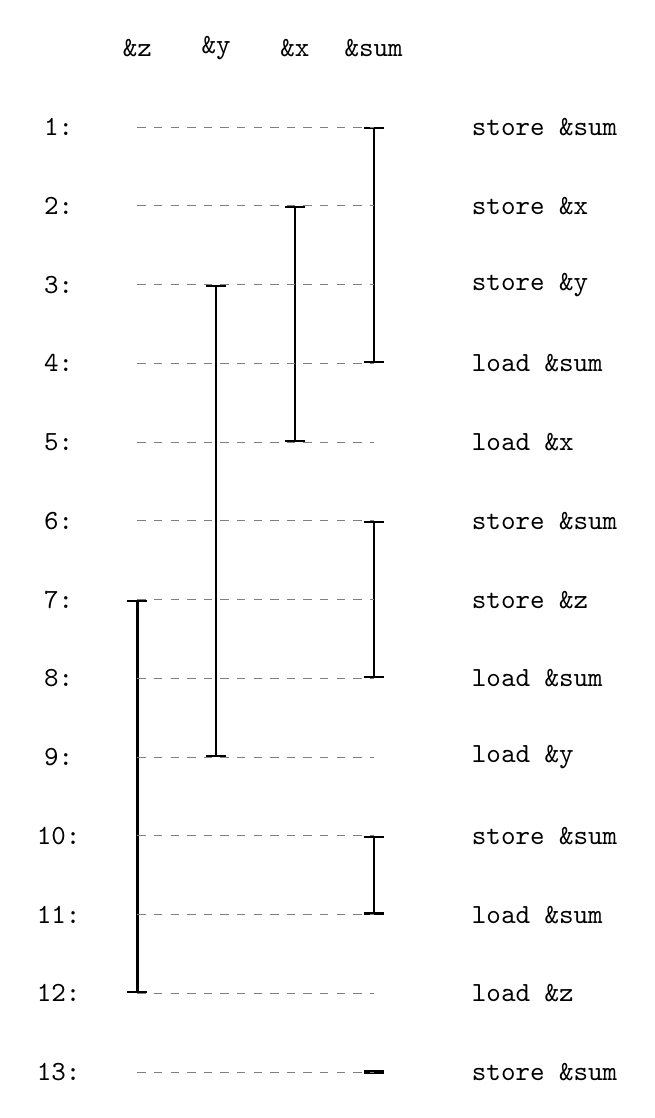
\begin{tikzpicture}

\node [align=left] at (0,0) {\texttt{\&sum}};
\node [align=left] at (-1,0) {\texttt{\&x}};
\node [align=left] at (-2,0) {\texttt{\&y}};
\node [align=left] at (-3,0) {\texttt{\&z}};

\draw [|-|][thick] (0,-1) -- (0,-4);
\draw [|-|][thick] (0,-6) -- (0,-8);
\draw [|-|][thick] (0,-10) -- (0,-11);
\draw [|-|][thick] (0,-13) -- (0,-13);
\draw [|-|][thick] (-1,-2) -- (-1,-5);
\draw [|-|][thick] (-2,-3) -- (-2,-9);
\draw [|-|][thick] (-3,-7) -- (-3,-12);

\node [label=right:\texttt{store \&sum}] at (1,-1)  {};
\node [label=right:\texttt{store \&x  }] at (1,-2)  {};
\node [label=right:\texttt{store \&y  }] at (1,-3)  {};
\node [label=right:\texttt{load  \&sum}] at (1,-4)  {};
\node [label=right:\texttt{load  \&x  }] at (1,-5)  {};
\node [label=right:\texttt{store \&sum}] at (1,-6)  {};
\node [label=right:\texttt{store \&z  }] at (1,-7)  {};
\node [label=right:\texttt{load  \&sum}] at (1,-8)  {};
\node [label=right:\texttt{load  \&y  }] at (1,-9)  {};
\node [label=right:\texttt{store \&sum}] at (1,-10) {};
\node [label=right:\texttt{load  \&sum}] at (1,-11) {};
\node [label=right:\texttt{load  \&z  }] at (1,-12) {};
\node [label=right:\texttt{store \&sum}] at (1,-13) {};

\foreach \y in {1,2,3,...,13}
{
  \node at (-4, -\y) {\texttt{\y:}};
  \draw [-][draw=gray,dashed] (-3, -\y) -- (0, -\y);
}
\end{tikzpicture}

  \caption{Liveness intervals of the C code example shown in \Cref{fig:mat-example-c-code}.}
  \label{fig:liveness-intervals-example}
\end{figure}

This section presented the definition of liveness and especially of liveness intervals.
The definition of liveness intervals is one of the most central components of this work.
It is the base for the trace transformations described in \Cref{sec:trace-transformation}.

%%%%%%%%%%%%%%%%%%%%%%%%%%%%%%%%%%%%%%%%%%%%%%%%%%%%%%%%%%%%%%%%%%%%%%%%%%%%%%%%%%%%%%%%%%%%%%%%%%%
% Performance
%%%%%%%%%%%%%%%%%%%%%%%%%%%%%%%%%%%%%%%%%%%%%%%%%%%%%%%%%%%%%%%%%%%%%%%%%%%%%%%%%%%%%%%%%%%%%%%%%%%

\section{Performance}\label{sec:performance}

This section presents how the performance of a trace is computed.
The performance of a trace is the most significant criteria of its quality.
In general \ac{trace}s with better performance use the memory available in a more efficient way than others.
The performance is independent of the number of instructions a \ac{trace} consists of.
The only important criteria is the number of memory accesses.
As \Cref{fig:hardware-model} shows there are different kinds of memory access.
Depending if the accessed address is in the cache or not the time required to load the value of a address into a register varies.
Cached data can be access much faster than data which has to be loaded from the main memory.
The \emph{latency} to load data into a register is measured in \emph{\ac{CPU} cycles}.
\ac{CPU} cycles are a common metric to measure durations at hardware level.

In our system \emph{performance} is expressed in \ac{CPA}.
Indeed performance is not directly measured.
As \Cref{equ:performance-cpa} illustrates it is computed according to the number of memory accesses that raised during execution.
\ac{CPA} describes the average number of \ac{CPU} cycles per memory access.
A memory access is equivalent to an instruction of the trace.

We proceed as follows, after the \ac{trace} of a program has been generated its performance is analyzed by applying the trace on a simulated cache and counting the different kinds of memory accesses.
At the end of the execution the performance is computed as illustrated by \Cref{equ:performance-cpa}.

\begin{equation}\label{equ:performance-cpa}
\text{CPA}(T,C) = \frac{\text{Sum of cycles}(T, C)}{\text{Sum of accesses}(T)}
\end{equation}

$T$ represents the \ac{trace} of the analyzed program.
$C$ represents the applied cache, the different caches are explained in \Cref{sec:caches}.

\emph{sum of cycles(T, C)} represents the sum of all memory accesses and each one weight according to its costs.
The costs for a memory access the depends on the latency of the memory unit that is accessed.
This is why cache accesses are cheaper than accessing the main memory.
The \emph{sum of accesses(T)} represents the total number of load and store instructions executed by the \ac{trace} $T$.

\Cref{tab:memory-access-cost} shows the costs for the different types of memory accesses.
These numbers are taken from literature \cite{drepper2007every}, \cite{skylake}.
The actual values are not that important than the relation of the costs.

\begin{table}[!ht]
  \centering
  \begin{tabular}{lc}
  \hline
  Memory Access Type & Cost in Cycles \\
  \hline
  Cache  load  & 1 \\
  Cache  store & 1 \\
  Memory load  & 5 \\
  Memory store & 5 \\
  \hline
  \end{tabular}
  \caption{Cost for memory access types}
  \label{tab:memory-access-cost}
\end{table}

This section presents our definition of performance and how the performance of a trace is computed.
For this procedure the memory accesses of a \ac{trace} are recored and finally used for computation.

%%%%%%%%%%%%%%%%%%%%%%%%%%%%%%%%%%%%%%%%%%%%%%%%%%%%%%%%%%%%%%%%%%%%%%%%%%%%%%%%%%%%%%%%%%%%%%%%%%%
% Metrics
%%%%%%%%%%%%%%%%%%%%%%%%%%%%%%%%%%%%%%%%%%%%%%%%%%%%%%%%%%%%%%%%%%%%%%%%%%%%%%%%%%%%%%%%%%%%%%%%%%%

\section{Metrics}\label{sec:metrics}

This section presents the metrics chosen to characterize a \ac{trace}.
The characteristic of \ac{trace} consists of the four metrics \emph{accesses}, \emph{access distance}, \emph{overlapping liveness}, and \emph{liveness interval length}.
These are used to reason about the resulting performance of a \ac{trace} and further to compare a \ac{trace} with other \ac{trace}s.
The metrics presented by this section are all applied after \ac{trace} transformation.
Hence, these operate on variables rather than directly on addresses.
Nevertheless, variables could easily be mapped to addresses.
Furthermore, for all four metrics the same statistical parameters are computed: minimum, maximum, average, 5\% percentile, 25\% percentile, 50\% percentile, 75\% percentile, and 95\% percentile.

\begin{remark} Statical metrics\
\begin{itemize}
\item The \emph{minimum} is the numerical smallest value of all samples.
\item The \emph{maximum} is the numerical largest value of all samples.
\item The \emph{average} is the arithmetic mean of all samples. It is computed by dividing the sum of all samples by the number of samples.
\item The \emph{percentile} is the value below which a given percentage of all samples fall, i.e., the 25\% percentile represents the value for which holds that 25\% of all samples are smaller than this value.
The $k$ percentile is computed by sorting all samples from smallest to largest.
Multiply the $k$ percent by the total number of values, this is the index within the sorted list of samples.
The $k$ percentile is the value at the computed index.
\end{itemize}
\end{remark}

\begin{figure}[!ht]
  \centering
  \begin{tabular}{c}
  \begin{lstlisting}
1: load  A
2: load  B
3: store A
  \end{lstlisting}
  \end{tabular}
  \caption{Tiny \ac{trace} example. Note: this trace has been transformed, i.e., there is no \texttt{\&} so \texttt{A} and \texttt{B} represent variables not addresses. On the left the instruction number is shown and on the right the correlating instruction is presented.}
  \label{fig:metrics-exmaple}
\end{figure}

\subsection{Accesses}\label{ssec:metric-accesses}
The metric called \emph{accesses} is as simple as the name suggests.
It investigates on the number of accesses on a certain variable.
For this reason the number of accesses on each variable are counted, regardless of the access type.
Applying this metric on the tiny example presented in \Cref{fig:metrics-exmaple} results in following list of samples $(1, 2)$.
Variable $A$ is accessed twice and variable $B$ is accessed only once.

\subsection{Access Distance}\label{ssec:metric-access-distance}
The \emph{access distance} metric shows the distance between two sequential accesses on the same variable.
For example if there is only one variable accessed the access distance of such a \ac{trace} is 0.
Assume a \ac{trace} that accesses two variables alternating as shown by \Cref{fig:metrics-access-distance-exmaple}, then the access distance of $A$ is 2.
Its computed by subtracting the instruction number of the current access and the instruction number of the previous access on a certain variable.
For example, the access distance of variable $A$ is computed by $3-1 = 2$, same of $B$ ($2 - 2 = 0$).
Applying this metric on the tiny example presented in \Cref{fig:metrics-exmaple} results in following list of samples $(0, 2)$.
Between the load of variable $A$ and the store on it there is only one other instruction, that the reason why there is $2$ in the list.
The $0$ results for variable $B$ that is accessed only once.

\subsection{Overlapping Liveness}\label{ssec:metric-concurrently-live}
The \emph{overlapping liveness} metric presents the number of variables that are live at a certain instruction number, the set of live variables is called \emph{working set}.
The term working set has been introduced by the work \cite{denning1968working}.
This metric shows how the working set of a \ac{trace}s grows and shrinks.
For this reason at each instruction the currently live variables are recorded.
Applying this metric on the tiny example presented in \Cref{fig:metrics-exmaple} results in following list of samples $(1, 1, 2)$.
At instruction number 1 and 3 only one variable is live $A$.
At instruction number 2 there are two variables live $A$, and $B$, respectively.

\subsection{Liveness Interval Length}\label{ssec:metric-liveness-interval-length}
The \emph{liveness interval length} metric illustrates the different lengths of liveness intervals.
In general a variable is used for a specific purpose that yields the variable to be live a certain timespan.
There are variables that are used for a short period and others are live for longer.
If a variable is only accessed once the liveness interval length is $0$.
The liveness interval length is computed similar to the access distance by subtracting the instruction number of beginning of a liveness interval from the instruction number of its last access.
Applying this metric on the tiny example presented in \Cref{fig:metrics-exmaple} results in following list of samples $(0, 2)$.
As explained above if a variable is only accessed once the liveness interval length is $0$, this is the case of $B$.
The length of the liveness interval of variable $A$ is represented by the second value of the list, $2$.

%%%%%%%%%%%%%%%%%%%%%%%%%%%%%%%%%%%%%%%%%%%%%%%%%%%%%%%%%%%%%%%%%%%%%%%%%%%%%%%%%%%%%%%%%%%%%%%%%%%
% Trace Transformation
%%%%%%%%%%%%%%%%%%%%%%%%%%%%%%%%%%%%%%%%%%%%%%%%%%%%%%%%%%%%%%%%%%%%%%%%%%%%%%%%%%%%%%%%%%%%%%%%%%%

\section{Trace Transformation}\label{sec:trace-transformation}

\Cref{sec:memory-access-trace} illustrated how to observe the \ac{trace} of a program.
\Cref{sec:liveness} describes our definition of liveness and introduces liveness intervals.
This section shows how to use these information to transform the \ac{trace} $T$ of a program.
The aim is to transform a \ac{trace} $T$ into a \ac{trace} $T'$ that is semantically equivalent to $T$, but offers better performance.
The performance of a \ac{trace} is determined as presented in \Cref{sec:performance}.
The transformation of a \ac{trace} does not effect the sequence of load and store instructions.
Nevertheless, the addresses used by the \ac{trace} are replaced according to a given algorithm.
The algorithms available are described below.
We distinguish the originally used addresses form the addresses used after transformation, the latter ones are called \emph{variables}.
We distinguishing the originally used addresses from those after transformation to emphasis the difference.
Further, it simplifies talking about \ac{trace}s.
Each time we talk about an address it refers to the \ac{trace} observed form the binary.
Talking about variables indicates that the \ac{trace} has been transformed already.

\subsection{Identity Trace}

The identity trace reproduces the original \ac{trace}.
For transformation each unique address of a \ac{trace} is replaced by an unique variable.
Based on the \ac{trace} (see \Cref{fig:mat-example-trace}) observed from the C code, illustrated in \Cref{fig:mat-example-c-code}, the addresses are replaces by variables, as shown in \Cref{fig:trace-transformation-original}.
Basically, \texttt{\&sum} becomes $A$, \texttt{\&x} becomes $B$, \texttt{\&y} becomes $C$, and \texttt{\&z} becomes $D$.
Obviously, there is one more difference the x-axis and y-axis are switched.
The reason is simple because it requires less space vertically.
However, note that liveness intervals of the variables shown in \Cref{fig:trace-transformation-original} are exactly the same as those of the addresses illustrated in \Cref{fig:liveness-intervals-example}.

\begin{figure}[!ht]
  \centering
  \begin{tikzpicture}

\node [align=left] at (0,0) {A};
\draw [|-|][thick] (1,0) -- (4,0);
\draw [|-|][thick] (6,0) -- (8,0);
\draw [|-|][thick] (10,0) -- (11,0);
\draw [|-|][thick] (13,0) -- (13,0);

\node [align=left] at (0,-1) {B};
\draw [|-|][thick] (2,-1) -- (5,-1);

\node [align=left] at (0,-2) {C};
\draw [|-|][thick] (3,-2) -- (9,-2);

\node [align=left] at (0,-3) {D};
\draw [|-|][thick] (7,-3) -- (12,-3);

\foreach \x in {1,2,3,...,13}
{
	\node at (\x,-7) {\x};
	\draw [-][draw=gray,dashed] (\x,-6.5) -- (\x,0.5);
}
\end{tikzpicture}

  \caption{Liveness intervals of the C code example shown in \Cref{fig:mat-example-c-code}.}
  \label{fig:trace-transformation-original}
\end{figure}

In this work two different kinds of \ac{trace} transformations are applied, expanding the \ac{trace} and collapsing the \ac{trace}.

\subsection{Single Assignment Trace}

The single assignment trace expands the original \ac{trace}, i.e., it uses more variables than the original \ac{trace} addresses.
For expanding a \ac{trace} we decided to use a \emph{single assignment} form.
More concrete each liveness interval of a \ac{trace} is assigned to a variable.
Further, a variable is never assigned a liveness interval more often than exactly once.
\Cref{fig:trace-transformation-sa} presents the \emph{single assignment trace} of \Cref{fig:mat-example-trace}.
It is not surprising that the number of variables required increases applying such an approach.
In detail, the four liveness intervals of address \texttt{\&sum} are know assigned to the variables $A$, $D$, $F$, and $G$.
In this example that variables are assigned in alphabetical order according to the beginning of an liveness interval.
This is the reason why the variables used to map the liveness intervals of address \texttt{\&sum} are not contiguous.
For this approach iterate through the \ac{trace} and each time a store instruction occurs assign the next free variable.
The implementation details are explained in \Cref{ssec:allocator-single-assignment}.

\begin{figure}[!ht]
  \centering
  \begin{tikzpicture}

\node [align=left] at (0,0) {A};
\draw [|-|][thick] (1,0) -- (4,0);

\node [align=left] at (0,-1) {B};
\draw [|-|][thick] (2,-1) -- (5,-1);

\node [align=left] at (0,-2) {C};
\draw [|-|][thick] (3,-2) -- (9,-2);

\node [align=left] at (0,-3) {D};
\draw [|-|][thick] (6,-3) -- (8,-3);

\node [align=left] at (0,-4) {E};
\draw [|-|][thick] (7,-4) -- (12,-4);

\node [align=left] at (0,-5) {F};
\draw [|-|][thick] (10,-5) -- (11,-5);

\node [align=left] at (0,-6) {G};
\draw [|-|][thick] (13,-6) -- (13,-6);

\foreach \x in {1,2,3,...,13}
{
  \node at (\x,-7) {\x};
  \draw [-][draw=gray,dashed] (\x,-6.5) -- (\x,0.5);
}
\end{tikzpicture}

  \caption{Liveness intervals of the C code example shown in \Cref{fig:mat-example-c-code} in \emph{single assignment} form.}
  \label{fig:trace-transformation-sa}
\end{figure}

\subsection{Compact Trace}

For collapsing a \ac{trace} we to use a \emph{compact} form.
More concrete each liveness interval of a \ac{trace} is assigned to a variable, but now variables are \emph{reused}.
If the liveness interval ends the variable is added to a \emph{free list}, i.e., a list of variable already use before but their liveness intervals already ended.
The procedure is as follows: before using a new variable the free list is checked, if there are variables available at the free list these are used.
Otherwise an new variable is assigned.
The implementation details are explained in \Cref{ssec:allocator-compact}.
There are various ways opportunities for the semantics of the free list.
In this work three variants are investigated, (1) stack semantic, (2) queue semantic, and (3) set semantic.
The set semantic is thought to represent a random selection of a free variable.
However, \Cref{fig:trace-transformation-compact} illustrates the compaction of the \ac{trace} shown in \Cref{fig:mat-example-trace} and applies a free list with stack semantics.
As expected this approach requires less variables.
The liveness intervals of \texttt{\&sum} remain the the same variable $A$.
Furthermore, the addresses \texttt{\&x} and \texttt{\&z} now share variable $B$.

\begin{remark}
Note that only by coexistent the liveness intervals of address \texttt{\&sum} are assigned to the same variable $A$.
In general is depends on the semantics of the free list and the currently free variables which variable a liveness interval is assigned to.
\end{remark}

\begin{figure}[!ht]
  \centering
  \begin{tikzpicture}

\node[align=left] at (0,0) {A};
\draw [|-|][thick] (1,0) -- (4,0);
\draw [|-|][thick] (6,0) -- (8,0);
\draw [|-|][thick] (10,0) -- (11,0);
\draw [|-|][thick] (13,0) -- (13,0);

\node [align=left] at (0,-1) {B};
\draw [|-|][thick] (2,-1) -- (5,-1);
\draw [|-|][thick] (7,-1) -- (12,-1);

\node [align=left] at (0,-2) {C};
\draw [|-|][thick] (3,-2) -- (9,-2);

\foreach \x in {1,2,3,...,13}
{
  \node at (\x,-7) {\x};
  \draw [-][draw=gray,dashed] (\x,-6.5) -- (\x,0.5);
}
\end{tikzpicture}

  \caption{Liveness intervals of the C code example shown in \Cref{fig:mat-example-c-code} in \emph{compacted} form.}
  \label{fig:trace-transformation-compact}
\end{figure}

This section presents two different kinds of \ac{trace} transformations, single assignment and compaction.
Single assignment potentially increases the number of used variables and compaction potentially decreases the number of used variables.

%%%%%%%%%%%%%%%%%%%%%%%%%%%%%%%%%%%%%%%%%%%%%%%%%%%%%%%%%%%%%%%%%%%%%%%%%%%%%%%%%%%%%%%%%%%%%%%%%%%
% Summarizing Example
%%%%%%%%%%%%%%%%%%%%%%%%%%%%%%%%%%%%%%%%%%%%%%%%%%%%%%%%%%%%%%%%%%%%%%%%%%%%%%%%%%%%%%%%%%%%%%%%%%%

\section{Summarizing Example}

Lets take a look at the performance of the three \ac{trace}s from above.
Assume a \ac{LRU} cache with 2 cache lines, each cache line fits exactly one variable.
For details on \ac{LRU} caches see \Cref{ssec:cache-lru}.
As a breath description of the applied cache, imaging as long as there is a free cache line within the cache, this one is used.
In case there is no more free cache line it is required to evict one of the used cache lines.
To make space the \emph{least recently used} cache line is evicted.

If a variable is accessed that is already in the cache a cheap cache access can be executed, either a load or store instruction.
Otherwise, the main memory has to be access that is much more expensive
The costs of the different kinds of accesses are presented in \Cref{tab:memory-access-cost}.
For the following performance computation we assume a simple optimization: the first store instruction on a variable can be executed directly into the cache.
Further, assume that in case of an eviction the data of a variable has to be stored in the main memory.
Regardless if the variable is still alive or already dead.

\subsection{Identity Trace}
\Cref{fig:trace-transformation-original-marked} shows the annotated liveness intervals of the identity \ac{trace} illustrated in \Cref{fig:trace-transformation-original}.
According to the assumptions from above every beginning of a liveness interval is annotated with a cache store.
Since the assumed cache fits exactly two variables the first eviction occurs when writing variable $C$ at instruction number 3.
According to the eviction policy of the applied \ac{LRU} cache variable $A$ is evicted.
The memory store of variable $A$ is annotated with a filled red circle.
Unfortunately, variable $A$ is accessed at the next instruction.
For this reason it has to be loaded from the main memory again, but before $B$ has to be stored in in the main memory to make space in the cache for $A$.
The same procedure repeats for the variables $B$ and $C$ at instruction number 5.
At instruction number 6 we are able to load a variable directly from cache for the first time.
Nevertheless, there are two more evictions required to finish the execution of this trace.
One at instruction number 7, variable $B$ is evicted to make space for variable $D$.
A interesting aspect at this instruction is that the liveness interval of variable $B$ ended two instructions before, hence $B$ is dead.
Furthermore, $B$ is not needed anymore for the following instructions.
In general this information is not available, this is the reason why there is a memory store annotated.
However, if a system knows about the liveness intervals of its variables it might decide to overwrite the value of $B$ with the value of $D$ and avoid the memory store.
The last eviction appears at instruction number 9, variable $C$ is accessed for the last time. Variable $A$ is accessed several time without any interaction with the main memory, because each time it is accessed it is in the cache.

\begin{figure}[!ht]
  \centering
  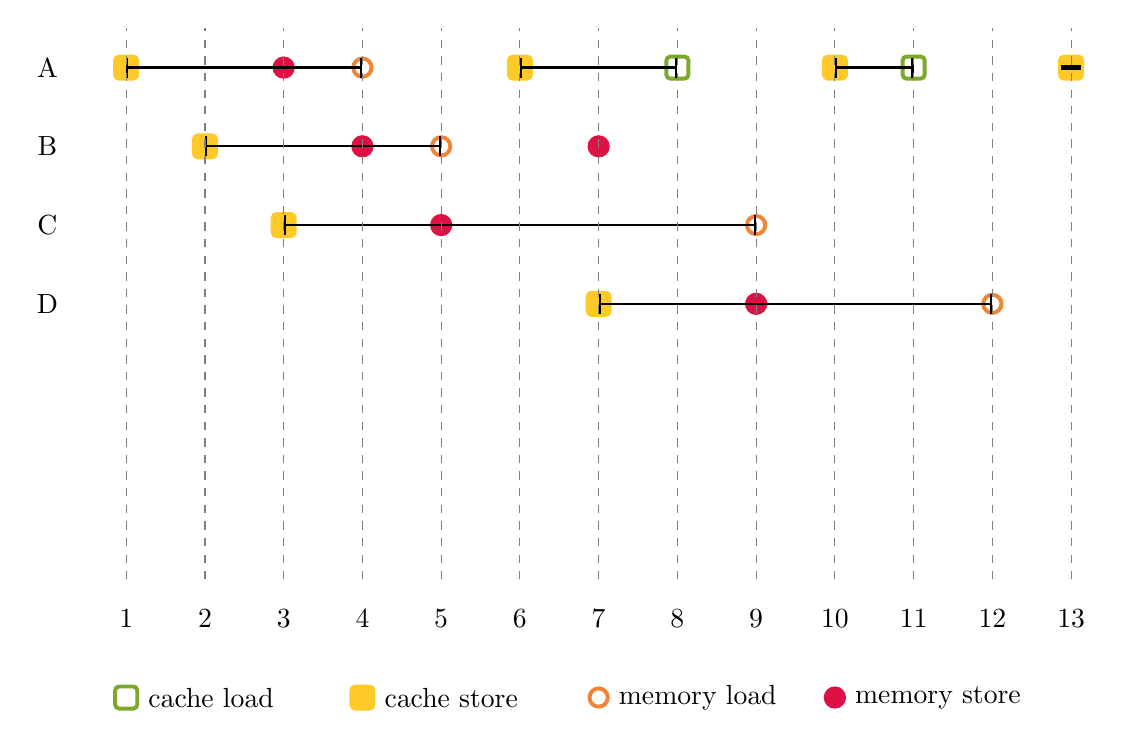
\begin{tikzpicture}

\node [align=left] at (0,0) {A};
\node[cache-store] at (1,0) {};
\node[memory-store] at (3,0) {};
\node[memory-load] at (4,0) {};
\node[cache-store] at (6,0) {};
\node[cache-load] at (8,0) {};
\node[cache-store] at (10,0) {};
\node[cache-load] at (11,0) {};
\node[cache-store] at (13,0) {};
\draw [|-|][thick] (1,0) -- (4,0);
\draw [|-|][thick] (6,0) -- (8,0);
\draw [|-|][thick] (10,0) -- (11,0);
\draw [|-|][thick] (13,0) -- (13,0);

\node [align=left] at (0,-1) {B};
\node[cache-store] at (2,-1) {};
\node[memory-store] at (4,-1) {};
\node[memory-load] at (5,-1) {};
\node[memory-store] at (7,-1) {};
\draw [|-|][thick] (2,-1) -- (5,-1);

\node [align=left] at (0,-2) {C};
\node[cache-store] at (3,-2) {};
\node[memory-store] at (5,-2) {};
\node[memory-load] at (9,-2) {};
\draw [|-|][thick] (3,-2) -- (9,-2);

\node [align=left] at (0,-3) {D};
\node[cache-store] at (7,-3) {};
\node[memory-store] at (9,-3) {};
\node[memory-load] at (12,-3) {};
\draw [|-|][thick] (7,-3) -- (12,-3);

\node[cache-load,   label=right:cache load]   at  (1,-8) {};
\node[cache-store,  label=right:cache store]  at  (4,-8) {};
\node[memory-load,  label=right:memory load]  at  (7,-8) {};
\node[memory-store, label=right:memory store] at (10,-8) {};

\foreach \x in {1,2,3,...,13}
{
	\node at (\x,-7) {\x};
	\draw [-][draw=gray,dashed] (\x,-6.5) -- (\x,0.5);
}
\end{tikzpicture}

  \caption{Liveness intervals of the C code example shown in \Cref{fig:mat-example-c-code}. Annotated by the different kinds of memory accesses. Assuming a LRU cache with 2 cache lines, each cache line fits exactly one variable.}
  \label{fig:trace-transformation-original-marked}
\end{figure}

The metrics of this \ac{trace} are illustrated in \Cref{fig:trace-transformation-original-marked}.
The \emph{accesses} metric is observed by recording the number of accesses for each variable.
In this example the list of samples holds four values one for each variable.
The number of accesses on variable $A$ is $7$, all other variables are accessed twice.
The resulting sorted list of samples looks as follows $(2, 2, 2, 7)$.
The \emph{access distance} presents a kind of the access frequency on an variable.
Depending on the number of accesses the list of access distances could be significantly larger than the number of used variables.
In this case the sorted list of samples looks as follows $(0, 1, 2, 2, 2, 2, 3, 3, 5, 6)$.
For variable $A$ there are multiple access distances (from left to write) $3$, $2$, $2$, $2$, $1$, and $0$.
The \emph{overlapping liveness} metrics shows how many variables are used at a certain instruction number.
The list of samples is computed by counting the overlapping liveness intervals for each instruction number.
As a result the size of the samples list depends on the number of instructions rather than on the number of used variables.
In case of the current example the samples are $(1, 2, 3, 3, 2, 2, 3, 3, 2, 2, 2, 1, 1)$.
For the purpose of better understanding the list is not sorted.
Instead it is ordered according to the correlating instruction number, i.e., the first entry represents the number of overlapping liveness intervals at instruction number 1.
The fourth metric is the \emph{liveness interval length}.
The number of used variables and the number of accesses on a variables define number of samples for this metric.
The number of accesses on a variable are significant, because these define the liveness intervals.
For this example the list of samples looks as follows $(0, 1, 2, 3, 3, 5, 6)$.
For variable $A$ there are four entry in the list $0$, $1$, $2$, and $3$.
The resulting metrics are presented in \Cref{tab:summarizing-example-metrics-original}.

\begin{table}[!ht]
  \centering
  \begin{tabular}{lrrrrrrrr}
    \hline
    \multirow{2}{*}{Metric} & \multirow{2}{*}{Min.} & \multirow{2}{*}{Max.} & \multirow{2}{*}{Avg.} & \multicolumn{5}{c}{Percentile} \tabularnewline
    & & & & 5\% & 25\% & 50\% & 75\% & 95\% \tabularnewline
    \hline
    Accesses                 & 2.00 & 7.00 & 3.25 & 2.00 & 2.00 & 2.00 & 3.25 & 6.25 \\
    Access Distance          & 0.00 & 6.00 & 2.60 & 0.45 & 2.00 & 2.00 & 3.00 & 5.55 \\
    Overlapping Liveness     & 1.00 & 3.00 & 2.08 & 1.00 & 2.00 & 2.00 & 3.00 & 3.00 \\
    Liveness Interval Length & 0.00 & 6.00 & 2.86 & 0.30 & 1.50 & 3.00 & 4.00 & 5.69 \\
    \hline
  \end{tabular}
  \caption{Metrics of the identity \ac{trace} illustrated in \Cref{fig:trace-transformation-original-marked} (values are rounded).}
  \label{tab:summarizing-example-metrics-original}
\end{table}

To compute the performance of \Cref{equ:trace-transformation-original-marked} the different kinds of memory access have to be counted and weight as illustrated by \Cref{equ:trace-transformation-original-marked}.
According to the annotations of \Cref{fig:trace-transformation-original-marked} there are 2 cache load, 7 cache stores, 4 memory loads, and 5 memory stores.
The result of this equation indicates that $4.15$ \ac{CPU} cycles are required in average to proceed one instruction of the \ac{trace}.

\begin{equation}\label{equ:trace-transformation-original-marked}
\text{\ac{CPA}}(T_{original}, C_{LRU}) = \frac{1 * (2 + 7) + 5 * (4 + 5)}{13} = 4.15
\end{equation}

\subsection{Single Assignment Trace}
\Cref{fig:trace-transformation-sa-marked} shows the annotated liveness intervals of the single assignment trace of \Cref{fig:trace-transformation-sa}.
Unexpectedly, the number of cache stores increases according to the number of variables used.
The combination of: using more variables and the assumption that the first access on a variable yields a cache store, increases the number of cache stores executed.
Further, using more variables seams to reduce the number of cache loads at least for this example.
In total the number of cache accesses is the same as for the identity \ac{trace}, but the distribution differs.
Taking a look at the main memory accesses we observe an increase in the number of memory stores.
The single assignment \ac{trace} requires the same amount of memory loads as the identity \ac{trace}.
Compared to \Cref{fig:trace-transformation-original} there are three times more memory stores on variables that are already dead.
The other four memory stores executed are identical to those of the identity \ac{trace}.

\begin{figure}
  \centering
  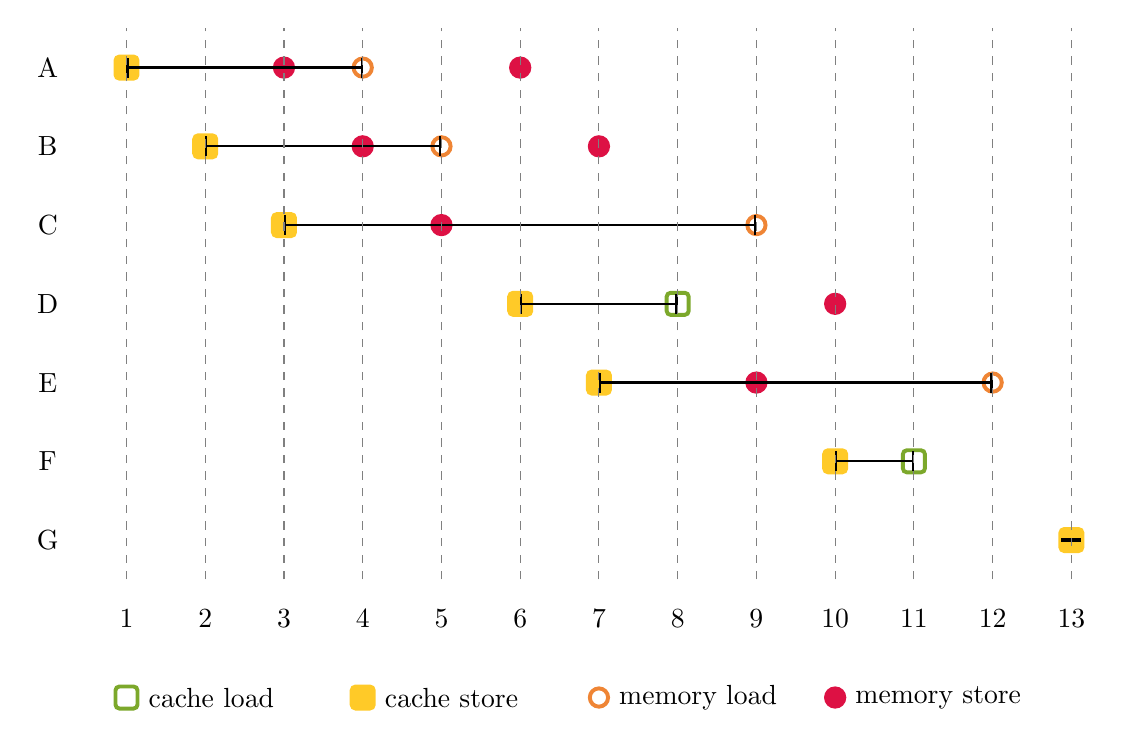
\begin{tikzpicture}

\node [align=left] at (0,0) {A};
\node[cache-store] at (1,0) {};
\node[memory-store] at (3,0) {};
\node[memory-load] at (4,0) {};
\node[memory-store] at (6,0) {};
\draw [|-|][thick] (1,0) -- (4,0);

\node [align=left] at (0,-1) {B};
\node[cache-store] at (2,-1) {};
\node[memory-store] at (4,-1) {};
\node[memory-load] at (5,-1) {};
\node[memory-store] at (7,-1) {};
\draw [|-|][thick] (2,-1) -- (5,-1);

\node [align=left] at (0,-2) {C};
\node[cache-store] at (3,-2) {};
\node[memory-store] at (5,-2) {};
\node[memory-load] at (9,-2) {};
\draw [|-|][thick] (3,-2) -- (9,-2);

\node [align=left] at (0,-3) {D};
\node[cache-store] at (6,-3) {};
\node[cache-load] at (8,-3) {};
\node[memory-store] at (10,-3) {};
\draw [|-|][thick] (6,-3) -- (8,-3);

\node [align=left] at (0,-4) {E};
\node[cache-store] at (7,-4) {};
\node[memory-store] at (9,-4) {};
\node[memory-load] at (12,-4) {};
\draw [|-|][thick] (7,-4) -- (12,-4);

\node [align=left] at (0,-5) {F};
\node[cache-store] at (10,-5) {};
\node[cache-load] at (11,-5) {};
\draw [|-|][thick] (10,-5) -- (11,-5);

\node [align=left] at (0,-6) {G};
\node[cache-store] at (13,-6) {};
\draw [|-|][thick] (13,-6) -- (13,-6);

\node[cache-load,   label=right:cache load]   at  (1,-8) {};
\node[cache-store,  label=right:cache store]  at  (4,-8) {};
\node[memory-load,  label=right:memory load]  at  (7,-8) {};
\node[memory-store, label=right:memory store] at (10,-8) {};

\foreach \x in {1,2,3,...,13}
{
  \node at (\x,-7) {\x};
  \draw [-][draw=gray,dashed] (\x,-6.5) -- (\x,0.5);
}
\end{tikzpicture}

  \caption{Liveness intervals of the C code example shown in \Cref{fig:mat-example-c-code} in \emph{single assignment} form. Annotated by the different kinds of memory accesses. Assuming a \ac{LRU} cache with 2 cache lines, each cache line fits exactly one variable.}
  \label{fig:trace-transformation-sa-marked}
\end{figure}

The accesses for the \ac{trace} shown in \Cref{fig:trace-transformation-sa} is computed as introduced in \Cref{ssec:metric-accesses}.
The computation outputs this list of samples: $(1, 2, 2, 2, 2, 2, 2)$.
As expected for each variable there is only one entry in the list.
Different to the accesses of the identity \ac{trace} there are more entries.
By coincident each variable except $G$ is accessed twice.
Computing the \emph{access distance} results in following list of samples $(0, 1, 2, 3, 3, 5, 6)$.
The \emph{overlapping liveness} variables are observed by counting the overlapping liveness intervals and result in the displayed list $(1, 2, 3, 3, 2, 2, 3, 3, 2, 2, 2, 1, 1)$.
Since the liveness intervals are not change during transforming a \ac{trace} these values are the same as for the identity \ac{trace}.
The samples for the \emph{liveness interval length} look as follows $(0, 1, 2, 3, 3, 5, 6)$.
For this example the samples of the access distance and the liveness interval length are identical, but this is a coincident.
\Cref{tab:summarizing-example-metrics-sa} presents the statistical metrics.

\begin{table}[!ht]
  \centering
  \begin{tabular}{lrrrrrrrr}
    \hline
    \multirow{2}{*}{Metric} & \multirow{2}{*}{Min.} & \multirow{2}{*}{Max.} & \multirow{2}{*}{Avg.} & \multicolumn{5}{c}{Percentile} \tabularnewline
    & & & & 5\% & 25\% & 50\% & 75\% & 95\% \tabularnewline
    \hline
    Accesses                 & 1.00 & 2.00 & 1.86 & 1.30 & 2.00 & 2.00 & 2.00 & 2.00 \\
    Access Distance          & 0.00 & 6.00 & 2.86 & 0.30 & 1.50 & 3.00 & 4.00 & 5.67 \\
    Overlapping Liveness.    & 1.00 & 3.00 & 2.08 & 1.00 & 2.00 & 2.00 & 3.00 & 3.00 \\
    Liveness Interval Length & 0.00 & 6.00 & 2.86 & 0.30 & 1.50 & 3.00 & 4.00 & 5.69 \\
    \hline
  \end{tabular}
  \caption{Metrics of the single assignment trace \ac{trace} illustrated by \Cref{fig:trace-transformation-sa-marked} (values are rounded).}
  \label{tab:summarizing-example-metrics-sa}
\end{table}

For this single assignment trace we observe 2 cache loads, 7 cache stores, 4 memory loads, and 7 memory stores that result in a \ac{CPA} of $4.92$.
This result is slightly worse than the \ac{CPA} of the identity \ac{trace} presented by \Cref{equ:trace-transformation-original-marked}.

\begin{equation}\label{equ:trace-transformation-sa-marked}
\text{\ac{CPA}}(T_{single~assigment}, C_{LRU}) = \frac{1 * (2 + 7) + 5 * (4 + 7)}{13} = 4.92
\end{equation}

\subsection{Compact Trace}
\Cref{fig:trace-transformation-compact-marked} shows the annotated liveness intervals of the compact trace based on \Cref{fig:trace-transformation-compact}.
The most significant difference compared to the others two traces is the number of variables used.
Variable $B$ is reused instead of picking a new variable.
Obviously, there are less memory stores required than for the single assignment trace.
Furthermore, there are even less memory stores required than for the identity \ac{trace}.
The reason is that reusing variable $B$ turns the memory store into a cache store.
The other memory accesses are quite similar as explained above.
Each liveness interval begins with a cache store.
Variable $A$ allows two cache loads.
The memory stores on the instruction numbers 3, 4, 5, and 9 are identical for all three traces.
Same for the memory loads at the instruction numbers 4, 5, 9, and 12.

\begin{figure}
  \centering
  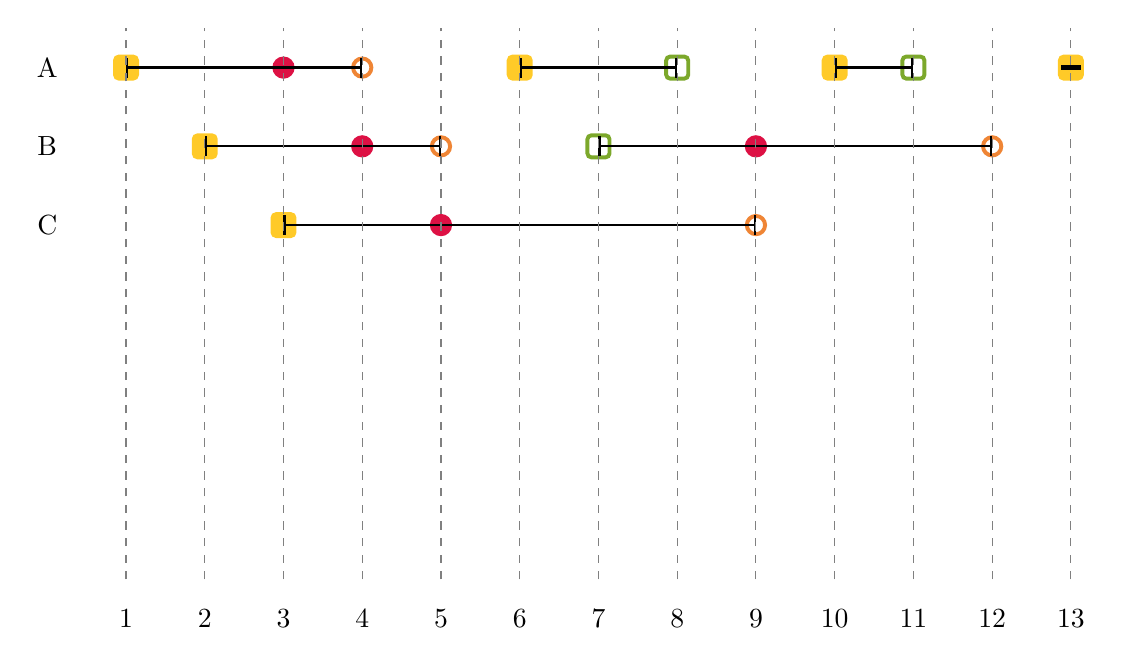
\begin{tikzpicture}

\node [align=left] at (0,0) {A};
\node[cache-store] at (1,0) {};
\node[memory-store] at (3,0) {};
\node[memory-load] at (4,0) {};
\node[cache-store] at (6,0) {};
\node[cache-load] at (8,0) {};
\node[cache-store] at (10,0) {};
\node[cache-load] at (11,0) {};
\node[cache-store] at (13,0) {};
\draw [|-|][thick] (1,0) -- (4,0);
\draw [|-|][thick] (6,0) -- (8,0);
\draw [|-|][thick] (10,0) -- (11,0);
\draw [|-|][thick] (13,0) -- (13,0);

\node [align=left] at (0,-1) {B};
\node[cache-store] at (2,-1) {};
\node[memory-store] at (4,-1) {};
\node[memory-load] at (5,-1) {};
\node[cache-load] at (7,-1) {};
\node[memory-store] at (9,-1) {};
\node[memory-load] at (12,-1) {};
\draw [|-|][thick] (2,-1) -- (5,-1);
\draw [|-|][thick] (7,-1) -- (12,-1);

\node [align=left] at (0,-2) {C};
\node[cache-store] at (3,-2) {};
\node[memory-store] at (5,-2) {};
\node[memory-load] at (9,-2) {};
\draw [|-|][thick] (3,-2) -- (9,-2);


\foreach \x in {1,2,3,...,13}
{
  \node at (\x,-7) {\x};
  \draw [-][draw=gray,dashed] (\x,-6.5) -- (\x,0.5);
}
\end{tikzpicture}

  \caption{Liveness intervals of the C code example shown in \Cref{fig:mat-example-c-code} in \emph{compacted} form. Annotated by the different kinds of memory accesses. Assuming a \ac{LRU} cache with 2 cache lines, each cache line fits exactly one variable.}
  \label{fig:trace-transformation-compact-marked}
\end{figure}

For the \ac{trace} presented in \Cref{fig:trace-transformation-compact} the list of samples for the \emph{accesses} metric is $(2, 4, 7)$.
According the number of used variables the list consists of three values.
The samples of the \emph{access distance} look as follows $(0, 1, 2, 2, 2, 2, 2, 3, 3, 5, 6)$.
The \emph{overlapping liveness} metrics yields in the same list of samples as for the identity \ac{trace} and the single assignment \ac{trace}, $(1, 2, 3, 3, 2, 2, 3, 3, 2, 2, 2, 1, 1)$.
Reason is that the liveness intervals are not changed only rearranged.
As already mentioned the samples for the \emph{liveness interval length} are the same as for the single assignment \ac{trace} and the identity \ac{trace}, $(0, 1, 2, 3, 3, 5, 6)$.
The reason for this is at the liveness intervals are never changed.
The resulting statistical metrics are presented by \Cref{tab:summarizing-example-metrics-compact}.

\begin{table}[!ht]
  \centering
  \begin{tabular}{lrrrrrrrr}
    \hline
    \multirow{2}{*}{Metric} & \multirow{2}{*}{Min.} & \multirow{2}{*}{Max.} & \multirow{2}{*}{Avg.} & \multicolumn{5}{c}{Percentile} \tabularnewline
    & & & & 5\% & 25\% & 50\% & 75\% & 95\% \tabularnewline
    \hline
    Accesses                 & 2.00 & 7.00 & 4.33 & 2.20 & 3.00 & 4.00 & 5.50 & 6.70 \\
    Access Distance          & 0.00 & 6.00 & 2.55 & 0.50 & 2.00 & 2.00 & 3.00 & 5.50 \\
    Overlapping Liveness     & 1.00 & 3.00 & 2.08 & 1.00 & 2.00 & 2.00 & 3.00 & 3.00 \\
    Liveness Interval Length & 0.00 & 6.00 & 2.86 & 0.30 & 1.50 & 3.00 & 4.00 & 5.69 \\
    \hline
  \end{tabular}
  \caption{Metrics of the compact trace \ac{trace} illustrated by \Cref{fig:trace-transformation-compact-marked} (values are rounded).}
  \label{tab:summarizing-example-metrics-compact}
\end{table}

There are 2 cache loads, 7 cache stores, 4 memory loads, and 4 memory stores required for the execution, that results in a \ac{CPA} of $3.77$.
This result the best one of the presented ones, that shows that for this example the presented compact trace performs best.

\begin{equation}\label{equ:trace-transformation-compact-marked}
\text{\ac{CPA}}(T_{compact}, C_{LRU}) = \frac{1 * (2 + 7) + 5 * (4 + 4)}{13} = 3.77
\end{equation}

\subsection{Conclusion}
To conclude the summarizing example for each metric and the performance the three \ac{trace}s are compared. This example concludes the Theoretical Foundations with illustrating the differences of the identical \ac{trace}, the single assignment \ac{trace} and the compact \ac{trace}.

\subsubsection{Performance}
\Cref{tab:summarizing-example-performance} presents the computed performance for each \ac{trace} applied to a simulated cache based on \ac{LRU} eviction policy.
As the table shows a transformation not always leads to an improvement.
For this example the compacted \ac{trace} yield the best performance.

\begin{table}[!ht]
  \centering
  \begin{tabular}{lrrrrrrrr}
    \hline
    Trace & \ac{CPA} \tabularnewline
    \hline
    Identity          & 4.15 \\
    Single Assignment & 4.92 \\
    Compact           & 3.77 \\
    \hline
  \end{tabular}
  \caption{Compare the \emph{performance} of all three different \ac{trace}s.}
  \label{tab:summarizing-example-performance}
\end{table}

\subsubsection{Accesses}

By transforming a \ac{trace} into another one the total number of accesses never changes.
Nevertheless, which variable and how many times it is accessed could be different.
\Cref{tab:summarizing-example-metrics-overview-accesses} illustrates the comparison of the three \ac{trace}s discussed.
Obviously, the variables of the single assignment \ac{trace} are accessed significantly less often than it is the case for the others.
To pick one value, 95 percentage of all variables of the single assignment \ac{trace} are accessed only twice.
For the identity \ac{trace} and the compact \ac{trace} the 95\% percentile is larger than 6.
Hence, the variables of the compact \ac{trace} and the identity \ac{trace} are accessed $\sim3$ times more often that those of the single assignment \ac{trace}.

\begin{table}[!ht]
  \centering
  \begin{tabular}{lrrrrrrrr}
    \hline
    \multirow{2}{*}{Trace} & \multirow{2}{*}{Min.} & \multirow{2}{*}{Max.} & \multirow{2}{*}{Avg.} & \multicolumn{5}{c}{Percentile} \tabularnewline
    & & & & 5\% & 25\% & 50\% & 75\% & 95\% \tabularnewline
    \hline
    Identity          & 2.00 & 7.00 & 3.25 & 2.00 & 2.00 & 2.00 & 3.25 & 6.25 \\
    Single Assignment & 1.00 & 2.00 & 1.86 & 1.30 & 2.00 & 2.00 & 2.00 & 2.00 \\
    Compact           & 2.00 & 7.00 & 4.33 & 2.20 & 3.00 & 4.00 & 5.50 & 6.70 \\
    \hline
  \end{tabular}
  \caption{Compare the \emph{accesses} metric of all three different \ac{trace}s.}
  \label{tab:summarizing-example-metrics-overview-accesses}
\end{table}

\subsubsection{Access Distance}

\Cref{tab:summarizing-example-metrics-overview-access-distance} shows the comparison of the access distance metric.
The differences between identity \ac{trace} and compact \ac{trace} are minimal.
The reason is that there is only one difference, the liveness interval of variable $D$ form the identity \ac{trace} s merged into variable $B$ of the compact \ac{trace}.
For the calculation this means that there is one sample more in the list of the compact \ac{trace}.
All other samples are identical to those the identity \ac{trace}.
The differences between identity \ac{trace} and single assignment \ac{trace} are a more significant.
The reason is that the access distance of the single assignment \ac{trace} is reduced to the liveness intervals.
In this case the list of sample for the single assignment \ac{trace} is shorter than the one of the identity \ac{trace}.

\begin{table}[!ht]
  \centering
  \begin{tabular}{lrrrrrrrr}
    \hline
    \multirow{2}{*}{Trace} & \multirow{2}{*}{Min.} & \multirow{2}{*}{Max.} & \multirow{2}{*}{Avg.} & \multicolumn{5}{c}{Percentile} \tabularnewline
    & & & & 5\% & 25\% & 50\% & 75\% & 95\% \tabularnewline
    \hline
    Identity          & 0.00 & 6.00 & 2.60 & 0.45 & 2.00 & 2.00 & 3.00 & 5.55 \\
    Single Assignment & 0.00 & 6.00 & 2.86 & 0.30 & 1.50 & 3.00 & 4.00 & 5.67 \\
    Compact           & 0.00 & 6.00 & 2.55 & 0.50 & 2.00 & 2.00 & 3.00 & 5.50 \\
    \hline
  \end{tabular}
  \caption{Compare the \emph{access distance} metric of all three different \ac{trace}s.}
  \label{tab:summarizing-example-metrics-overview-access-distance}
\end{table}

\subsubsection{Overlapping Liveness}
The results for the overlapping liveness metric are presented in \Cref{tab:summarizing-example-metrics-overview-concurrently-live}.
Unexpectedly, the results for all three \ac{trace}s are identical.
Hence, the liveness intervals are not modified by any transformation.

\begin{table}[!ht]
  \centering
  \begin{tabular}{lrrrrrrrr}
    \hline
    \multirow{2}{*}{Trace} & \multirow{2}{*}{Min.} & \multirow{2}{*}{Max.} & \multirow{2}{*}{Avg.} & \multicolumn{5}{c}{Percentile} \tabularnewline
    & & & & 5\% & 25\% & 50\% & 75\% & 95\% \tabularnewline
    \hline
    Identity          & 1.00 & 3.00 & 2.08 & 1.00 & 2.00 & 2.00 & 3.00 & 3.00 \\
    Single Assignment & 1.00 & 3.00 & 2.08 & 1.00 & 2.00 & 2.00 & 3.00 & 3.00 \\
    Compact           & 1.00 & 3.00 & 2.08 & 1.00 & 2.00 & 2.00 & 3.00 & 3.00 \\
    \hline
  \end{tabular}
  \caption{Compare the \emph{overlapping liveness} metric of all three different \ac{trace}s.}
  \label{tab:summarizing-example-metrics-overview-concurrently-live}
\end{table}

\subsubsection{Liveness Interval Length}
The results for the liveness interval length metric does not show any differences between the three \ac{trace}s as \Cref{tab:summarizing-example-metrics-overview-liveness-interval-length} illustrates.
It is as expected, because the liveness intervals are not modified by any transformation.

\begin{table}[!ht]
  \centering
  \begin{tabular}{lrrrrrrrr}
    \hline
    \multirow{2}{*}{Trace} & \multirow{2}{*}{Min.} & \multirow{2}{*}{Max.} & \multirow{2}{*}{Avg.} & \multicolumn{5}{c}{Percentile} \tabularnewline
    & & & & 5\% & 25\% & 50\% & 75\% & 95\% \tabularnewline
    \hline
    Identity          & 0.00 & 6.00 & 2.86 & 0.30 & 1.50 & 3.00 & 4.00 & 5.69 \\
    Single Assignment & 0.00 & 6.00 & 2.86 & 0.30 & 1.50 & 3.00 & 4.00 & 5.69 \\
    Compact           & 0.00 & 6.00 & 2.86 & 0.30 & 1.50 & 3.00 & 4.00 & 5.69 \\
    \hline
  \end{tabular}
  \caption{Compare the \emph{liveness interval length} metric of all three different \ac{trace}s.}
  \label{tab:summarizing-example-metrics-overview-liveness-interval-length}
\end{table}

%%%%%%%%%%%%%%%%%%%%%%%%%%%%%%%%%%%%%%%%%%%%%%%%%%%%%%%%%%%%%%%%%%%%%%%%%%%%%%%%%%%%%%%%%%%%%%%%%%%
%%%%%%%%%%%%%%%%%%%%%%%%%%%%%%%%%%%%%%%%%%%%%%%%%%%%%%%%%%%%%%%%%%%%%%%%%%%%%%%%%%%%%%%%%%%%%%%%%%%
%%%%%%%%%%%%%%%%%%%%%%%%%%%%%%%%%%%%%%%%%%%%%%%%%%%%%%%%%%%%%%%%%%%%%%%%%%%%%%%%%%%%%%%%%%%%%%%%%%%
%%%%%%%%%%%%%%%%%%%%%%%%%%%%%%%%%%%%%%%%%%%%%%%%%%%%%%%%%%%%%%%%%%%%%%%%%%%%%%%%%%%%%%%%%%%%%%%%%%%

%%%%%%%%%%%%%%%%%%%%%%%%%%%%%%%%%%%%%%%%%%%%%%%%%%%%%%%%%%%%%%%%%%%%%%%%%%%%%%%%%%%%%%%%%%%%%%%%%%%
% Problem Statement
%%%%%%%%%%%%%%%%%%%%%%%%%%%%%%%%%%%%%%%%%%%%%%%%%%%%%%%%%%%%%%%%%%%%%%%%%%%%%%%%%%%%%%%%%%%%%%%%%%%

\chapter{Problem Statement}\label{cha:problems-tatement}
\begin{definition}[Problem statement]
Given a \ac{trace} $T$ of load and store instructions find metrics that characterize the trace performance for a given cache $C$ and implement an execution engine for computing their quantities.
\end{definition}

%%%%%%%%%%%%%%%%%%%%%%%%%%%%%%%%%%%%%%%%%%%%%%%%%%%%%%%%%%%%%%%%%%%%%%%%%%%%%%%%%%%%%%%%%%%%%%%%%%%
%%%%%%%%%%%%%%%%%%%%%%%%%%%%%%%%%%%%%%%%%%%%%%%%%%%%%%%%%%%%%%%%%%%%%%%%%%%%%%%%%%%%%%%%%%%%%%%%%%%
%%%%%%%%%%%%%%%%%%%%%%%%%%%%%%%%%%%%%%%%%%%%%%%%%%%%%%%%%%%%%%%%%%%%%%%%%%%%%%%%%%%%%%%%%%%%%%%%%%%
%%%%%%%%%%%%%%%%%%%%%%%%%%%%%%%%%%%%%%%%%%%%%%%%%%%%%%%%%%%%%%%%%%%%%%%%%%%%%%%%%%%%%%%%%%%%%%%%%%%

\chapter{Implementation}\label{cha:implementation}

This chapter explains the implementation of our environment used for the experiments presented by \Cref{cha:experiment}. \Cref{cha:theoretical-foundations} explains the theoretical background for the tool chain applied to observe the aimed information. In general there are two major aspects we are interested in, (1) the performance of a \ac{trace} and (2) the metrics of a \ac{trace} which characterize its performance.

%%%%%%%%%%%%%%%%%%%%%%%%%%%%%%%%%%%%%%%%%%%%%%%%%%%%%%%%%%%%%%%%%%%%%%%%%%%%%%%%%%%%%%%%%%%%%%%%%%%
% Workflow
%%%%%%%%%%%%%%%%%%%%%%%%%%%%%%%%%%%%%%%%%%%%%%%%%%%%%%%%%%%%%%%%%%%%%%%%%%%%%%%%%%%%%%%%%%%%%%%%%%%

\section{Workflow}

We implemented a multistate offline approach to observe all the information as illustrated by \Cref{fig:workflow}. In this context \emph{offline} indicates that there are analyzing steps required before executing the \ac{trace}. More concrete this is about \emph{Preparation}, and \emph{Transformation \& Analysis}.

\begin{description}
  \item[Compilation] It is required to generate a binary of a benchmark which should be analyzed. The benchmarks we used are presented by \Cref{sec:benchmarks}. For our experiments these benchmarks are compiled with \emph{GCC 4.8.5} on \emph{Ubuntu 16.04} for \emph{AMD Opteron\texttrademark Processor 6376} with \emph{x86\_64 Architecture}.

  \item[Preparation] Next is to obtain a \ac{trace} of load and store instruction on addresses. We use the Valgrind\cite{Valgrind} tool called \emph{Lackey} to obtain all the memory accesses of an x86\_64 executable. This represents the \ac{trace} of the benchmark which will be analyzed and transformed later on.

  \item[Analysis] After the \ac{trace} has been obtained and before it is executed there is an analyzing step to observing the metrics explained in \Cref{sec:metrics}. This informations are partly used by some of the caches presented by \Cref{sec:caches}.

  \item[Execution \& Transformation] Finally the \ac{trace} can be executed to figure out its performance. During execution the \ac{trace} is transformed. An allocator is used to proceed the transformation into a single assignment \ac{trace}, or a compact \ac{trace}, or an identity \ac{trace}. This procedure requires to apply a cache. In this work there are several caches available which are presented by \Cref{sec:caches}. During execution the memory accesses are counted which are finally used to calculate the performance.
\end{description}

\begin{figure}[!ht]
  \centering
  \begin{tikzpicture}[every text node part/.style={align=center}]
%
% text of boxes
%
% benchmark
\newcommand{\bmkLabel}{benchmark (C/C++ code)}
\newcommand{\bmkContent}{\dots \\ \texttt{s = s + 1} \\ \dots}
% compilation
\newcommand{\comLabel}{x86\_64 binary}
\newcommand{\comContentAssembly}{%
    \\ \dots \\\texttt{movl -12(\%rbp), \%eax} \\ \texttt{addl \%eax, -16(\%rbp)} \\ \dots \\}
\newcommand{\comContentBinary}{\\ \dots \\ \texttt{010101010101} \\ \dots \\}
% memory access trace
\newcommand{\matLabel}{memory access trace}
\newcommand{\matContent}{%
  \dots \\ \texttt{load \&s} \\ \texttt{load \&x} \\ \texttt{store \&s} \\ \dots}
% trace transformation
\newcommand{\trtLabel}{transformed trace}
\newcommand{\trtContent}{\dots \\ \texttt{load A} \\ \texttt{load B} \\ \texttt{store A} \\ \dots}
%
% style
%
\tikzstyle{innernode}=[minimum width=4.5cm, node distance=0.25cm]
\tikzstyle{firstinnernode}=[minimum width=4.5cm, node distance=1.5cm]
\tikzstyle{outernode}=[minimum width=5.5cm]
%
% bmk
%
\node (bmk label)   [innernode]                                           {\bmkLabel};
\node (bmk content) [innernode, below=of bmk label]                       {\bmkContent};
\node (bmk)         [stdnode, outernode, fit={(bmk label) (bmk content)}] {};
%
% compilcation
%
\node (com label) [firstinnernode,     below=of bmk content.south]            {\comLabel};
\node (com ass)   [stdnode, innernode, below=of com label]                    {\comContentAssembly};
\node (com bin)   [stdnode, innernode, below=of com ass.south]                {\comContentBinary};
\node (com)       [stdnode, outernode, fit={(com label) (com ass) (com bin)}] {};
%
% memory access trace
%
\node (mat label)   [firstinnernode, below=of com bin.south]              {\matLabel};
\node (mat content) [innernode,      below=of mat label]                  {\matContent};
\node (mat)         [stdnode, outernode, fit={(mat label) (mat content)}] {};
%
% transformed trace
%
\node (trt label)   [firstinnernode, below=of mat content.south]          {\trtLabel};
\node (trt content) [innernode,      below=of trt label]                  {\trtContent};
\node (trt)         [stdnode, outernode, fit={(trt label) (trt content)}] {};

% % arrows
\draw [arrow, label] (com ass) -- (com bin);
\draw [arrow] (bmk) -- (com);
\draw [arrow] (com) -- (mat);
\draw [arrow] (mat) -- (trt);

\node [below=of bmk.south, yshift=0.7cm, xshift=1.5cm] {compilation};
\node [below=of com.south, yshift=0.7cm, xshift=1.5cm] {preparation};
\node [below=of mat.south, yshift=0.9cm, xshift=1.5cm] {execution \& \\ transformation};
\end{tikzpicture}

  \caption{Workflow}
  \label{fig:workflow}
\end{figure}

%%%%%%%%%%%%%%%%%%%%%%%%%%%%%%%%%%%%%%%%%%%%%%%%%%%%%%%%%%%%%%%%%%%%%%%%%%%%%%%%%%%%%%%%%%%%%%%%%%%
% Allocators
%%%%%%%%%%%%%%%%%%%%%%%%%%%%%%%%%%%%%%%%%%%%%%%%%%%%%%%%%%%%%%%%%%%%%%%%%%%%%%%%%%%%%%%%%%%%%%%%%%%

\section{Allocators}
\label{sec:allocators}

This section presents the implementation of the trace transformation. In general for every trace there is a transformation required to replace the addresses observed via Valgrind by variables. Even for analyzing the identity \ac{trace} this transformation is necessary. The actual transformation is done during the execution phase by an \emph{allocator}. Each store instruction is interpreted like a \texttt{malloc} in C. Hence, each store instruction forces the allocator to return an variable to operate on. This is the point in time where an address is replaced by a variable.  It is up to the used allocator if a new variable is returned or a variable is reused. This architecture is the reason why also for the execution the identity \ac{trace} a transformation is applied. In our system there are three types of allocators: the \emph{Identity Allocator}, the \emph{Single Assignment Allocator} and the \emph{Compact Allocator}.

\subsection{Identity Allocator}\label{ssec:allocator-original}

The identity allocator is used to measure the performance of a programs \ac{trace} with any chances. This allocator produces the \emph{identity \ac{trace}} as explained by \Cref{sec:trace-transformation}. The identity \ac{trace} is important to figure out which one of the other transformations shows an improvement and which make performance even worse. The implementation of the identity allocator is as simple as it simply used the addresses of a \ac{trace} as variables.

\subsection{Single Assignment Allocator}\label{ssec:allocator-single-assignment}

The single assignment allocator is used to illustrate the performance of never reusing any address at all. Which can be interpreted as compacting allocator with a compaction ration of 0 percentage. Which means there is no compaction. It is implemented by a bump pointer allocator assuming endless memory. Each time there is a store instruction the bump pointer is increased and the new variable is returned. The bump pointer is never decreased.

\subsection{Compacting Allocator}\label{ssec:allocator-compact}

The compacting allocators are used to illustrate the advantages and disadvantages of compaction. Compaction is achieved by using a free list. If the free list is empty the bump pointer is increased an the new variable is returned. Otherwise a variable of the free list is taken. The variable is removed from the list and return for usage. This work presents three different implementation of the compact allocator. These differ in the semantics of the free list, there is one implementation with \emph{stack} semantic, one with \emph{queue} semantic, and one with \emph{set} semantic. The stack semantic is equivalent with picking the most recently freed variable. In contract to the stack semantic there is the queue semantics which represents pick the least recently freed variable. And finally the set semantic represents picking a random variable of the freed ones.

%%%%%%%%%%%%%%%%%%%%%%%%%%%%%%%%%%%%%%%%%%%%%%%%%%%%%%%%%%%%%%%%%%%%%%%%%%%%%%%%%%%%%%%%%%%%%%%%%%%
% Caches
%%%%%%%%%%%%%%%%%%%%%%%%%%%%%%%%%%%%%%%%%%%%%%%%%%%%%%%%%%%%%%%%%%%%%%%%%%%%%%%%%%%%%%%%%%%%%%%%%%%

\section{Caches}\label{sec:caches}

This section presents our implementations of caches. As explained by \Cref{sec:hardware-model} within the environment of computer where \ac{CPU} communicates with the main memory a cache is a hardware component. For the purpose of this work all caches simulated are implemented in software. This allows us to analyze multiple different caches. Obviously, we cannot measure real time for the execution of \ac{trace} because every component of our environment is implement in software. This is the reason why in \Cref{sec:performance} the performance is defined by the number of different memory accesses instead of using the total execution time of a benchmark as usually.

Nevertheless, our cache implementations offer the most basic properties as configurable parameters.
For all implementations the \emph{cache size} and the \emph{cache line size} is configurable.
The \ac{LRU} caches offer several more configurable parameters.

\begin{remark}
Note that our cache implementations operate on variables rather than on addresses. This is because the applied allocator transforms the \ac{trace} of addresses into a \ac{trace} of variables.
\end{remark}

In our environment four caches are available. There two different eviction policies implemented. One using the classical \ac{LRU} algorithm to decide which item of the cache will be evicted. And the other one using an algorithm proposed by \Citeauthor{belady1966study} in his work \cite{belady1966study} from \citeyear{belady1966study} to decide on the item which will be evicted.

For both algorithms used as eviction policy there is another implementation which has full information about the liveness intervals of all variables of a \ac{trace}. This enables further optimizations as explained below.

\subsection{MIN Cache}\label{ssec:cache-MIN}

This implementation of a cache is based on the algorithm proposed in \cite{belady1966study}, called \emph{\ac{MIN}}. The basic idea behind \citeauthor{belady1966study}s algorithm is to evict the item within the cache which is not need for the longest time. More precise if there is a dead item in the cache evict it otherwise evict the item which is accessed again furthest in future. In praxis this algorithm is hard to apply, because it would require to know the future which is not the case in real systems. Nevertheless, analyzing an implementation of this approach is quite interesting, because the algorithm has been proofed to be the optimal eviction policy (\cite{mattson1970evaluation}, \cite{van2007short}, \cite{vogler2008another}, \cite{lee2016simple}). Even if this algorithm is hardly applicable in reality our environment offers all requirements. This is one advantage of the offline analysis of a \ac{trace}. All required information for the \citeauthor{belady1966study} algorithm is already available before the execution begins.

\subsection{Least Recently Used Cache}\label{ssec:cache-lru}

This implementation of a cache is based on the \ac{LRU} algorithm, which is part of the literature since years (\cite{johnson1994x3}, \cite{drepper2007every}, \cite{patterson2011computer}, \cite{jacob2010memory}, and many more). Different than \citeauthor{belady1966study}s algorithm the \ac{LRU} approach is widely used in praxis. Instead of caring about future access which are unknown in realty this approach takes a look at the pasted accesses. For this reason it is required to keep track of the accesses on the currently cache items. A \ac{LRU} cache decides based on its track information and always decided on the item in the cache which has not been accessed for the longest time. The is also the source of its name, \emph{least recently used}. The idea behind is that is an item has not been accessed for longer there is a possibility that it is not need anymore but still is in the cache. For the purpose of this work the \ac{LRU} cache implementation which comes with Valgrind is used.

\subsection{Cache Proceeding}
\subsubsection{Without Liveness Information}\label{ssec:cache-behavior}

The proceeding of a cache without liveness information in general is identical for the \ac{LRU} implantation and the \Citeauthor{belady1966study} implementation. The only difference is in the chose of the eviction candidate.

\begin{figure}[!ht]
  \centering
  \begin{tikzpicture}
  \node [block                               ] (init)       {access variable};
  \node [decision,        below=of init      ] (cached)     {cached?};
  \node [block,           below=of cached    ] (cache-miss) {cache miss};
  \node [block,           right=of cache-miss] (cache-hit)  {cache hit};
  \node [decision,        below=of cache-miss] (cache-full) {cache-full?};
  \node [block,           below=of cache-full] (eviction)   {eviction};
  \node [block-mem-store, below=of eviction  ] (store)      {memory store};
  \node [block-mem-load,  below=of store     ] (load)       {memory load};
  \node [block,           below=of load      ] (access)     {execute access};

  \node [corner,          left=of eviction   ] (c1) {};
  \node [corner,          left=of load       ] (c2) {};

  \path [line] (init)       -- (cached);
  \path [line] (cache-miss) -- (cache-full);
  \path [line] (cache-hit)  |- (access);
  \path [line] (eviction)   -- (store);
  \path [line] (store)      -- (load);
  \path [line] (load)       -- (access);

  \path [line] (cached)     -| node [below, near start] {yes} (cache-hit);
  \path [line] (cached)     -- node [right, near start] {no}  (cache-miss);

  \path [line] (cache-full) -- node [left,  near start] {yes} (eviction);
  \path [line] (cache-full) -| node [below, near start] {no}  (c1.south) -- (c2.north) |- (load);
\end{tikzpicture}

  \caption{Cache behavior without liveness information}
  \label{fig:cache-behavior}
\end{figure}

\Cref{fig:cache-behavior} illustrates proceeding of the caches. Everything starts with the access on a variable. Right now it does not matter if the access is a load or a store instruction. At first it is checked if the accessed variable is currently in the cache. In case the variable is cached, this is a cache hit, we are done and the initial access could be executed without any further actions.
Otherwise, if the accessed variable is not cached it is a cache miss. Such a case requires further action, namely the next step is to control if there is space for at least one more variable in the cache.

If the cache is full it is required to make some space. This is achieved by applying the eviction policy to decide on the variable which will be kicked out of the cache. The eviction candidates value has to be saved, for this reason its value is written back to main memory by a store instruction. Then, the accessed variables value can be loaded from main memory and finally the requested access can be executed.

In case that the cache is not full we are able to skip the selection of an eviction candidate and of course it is not required to save its value in main memory, so also the store instruction is not needed. Such a situation allows to immediately load the value of the requested variable. In this case an expensive store instruction on the main memory is saved.

Summarizing, in the worst case it is required to execute two expensive main memory instruction before the actual variable can be accessed. This is not optimal in comparison to the best case which does not require to access the main memory at all. However, as \Cref{fig:cache-behavior} illustrates there is the possibility get rid of at least one of the expensive instructions.

\subsubsection{With Liveness Information}\label{ssec:cache-behavior-liveness}

\Cref{ssec:cache-behavior} shows that there are certain cases in which the number of expensive main memory accesses can be reduced. This sections tries to minimize the number of main memory accesses by using the information about the liveness intervals of a \ac{trace}. Again the \ac{LRU} implementation and the \Citeauthor{belady1966study} implementation differ only by the selection of the eviction candidate.

\begin{figure}[!ht]
  \centering
  \scalebox{0.8}{\begin{tikzpicture}
  \node [block]                                (init)       {access variable};
  \node [decision,        below=of init]       (cached)     {cached?};
  \node [block,           below=of cached]     (cache-miss) {cache miss};
  \node [block,           right=of cache-miss] (cache-hit)  {cache hit};
  \node [decision,        below=of cache-miss] (cache-full) {cache-full?};
  \node [block,           below=of cache-full] (eviction)   {eviction};
  \node [decision,        below=of eviction]   (is-live)    {live?};
  \node [block-mem-store, below=of is-live]    (store)      {memory store};
  \node [inline-corner,   below=of store]      (c0)         {};
  \node [decision,        below=of c0]         (is-load)    {load?};
  \node [block-mem-load,  below=of is-load]    (load)       {memory load};
  \node [block,           below=of load]       (access)     {execute access};

  \node [corner,          left=of eviction                 ] (c1) {};
  \node [corner,          left=of c0,        xshift=-0.85cm] (c2) {};
  \node [corner,          right=of is-live,                ] (c3) {};
  \node [corner,          right=of c0,       xshift=+0.85cm] (c4) {};
  \node [corner,          left=of is-load,                 ] (c5) {};

  \path [line] (init)       -- (cached);
  \path [line] (cache-miss) -- (cache-full);
  \path [line] (cache-hit)  |- (access);
  \path [line] (eviction)   -- (is-live);
  \path [line] (store)      -- (c0);
  \path [line] (c0)         -- (is-load);
  \path [line] (load)       -- (access);

  \path [line] (cached)     -| node [below, near start] {yes} (cache-hit);
  \path [line] (cached)     -- node [right, near start] {no}  (cache-miss);

  \path [line] (cache-full) -- node [left,  near start] {yes} (eviction);
  \path [line] (cache-full) -| node [below, near start] {no}  (c1.south) -- (c2.north) |- (c0);

  \path [line] (is-live)    -- node [right, near start] {yes} (store);
  \path [line] (is-live)    -| node [below, near start] {no}  (c3.south) -- (c4.north) |- (c0);

  \path [line] (is-load)    -- node [left, near start] {yes} (load);
  \path [line] (is-load)    -| node [below, near start] {no}  (c5.south) |- (access);
\end{tikzpicture}
}
  \caption{Cache behavior with liveness information}
  \label{fig:cache-behavior-liveness}
\end{figure}

\Cref{fig:cache-behavior-liveness} illustrates the proceeding for caches with liveness informations. Everything starts with the access on a variable. By now it does not matter which kind of access it is. In case it becomes relevant it will be discussed. As without liveness information the first thing to do is to check if the accessed variable is already in the cache. If this is the case it is a cache hit and we are done. The actual access can be executed directly on the cache.
Otherwise, if the accessed variable is not in the cache yet, its a cache miss. A cache miss requires further steps to get the accessed variable into the cache.

Next is to check either the cache is full or not. In case there is no more space in the cache for another variable it is necessary to evict one of the cached variables. The eviction candidate is chosen by the eviction policy of the cache, either via \ac{LRU} algorithm or via \Citeauthor{belady1966study}s algorithm. In proceeding a variable access, the selection of the eviction candidate is the only difference which might occur between the two available implementations which use liveness information. Next, we make use of the liveness information by proofing if the eviction candidate is live or dead. If the eviction candidate is still live, this means its liveness interval did not end yet, it is necessary to save the variables value. For this reason a store instruction on main memory is executed to save the eviction candidates value. If the variable chosen for eviction is dead it is not required to save its value, because it is not used anymore in future. This is why the store instruction on main memory can be skipped.
If the cache is not full yet then the whole eviction procedure, selecting a variable to evict and saving its value if needed, can be skipped.

After all the possible steps and opportunities so far the cache reached a state in which there is at least one free spot available for the accessed variable. Only question remaining is do we have to load the accessed variable from main memory? This is the point in the whole procedure where the type of access on the currently accessed variable matters. In case of a load an main memory load instruction is yield. This is required to load the value written by one of the previous accessed. In case of a store on the currently accessed variable, its previously stored value does not matter any because its overwritten anyway. For this reason the expensive load instruction on main memory can be skipped.

And finally, we are able to execute the actual access on the variable directly on the cache.

%%%%%%%%%%%%%%%%%%%%%%%%%%%%%%%%%%%%%%%%%%%%%%%%%%%%%%%%%%%%%%%%%%%%%%%%%%%%%%%%%%%%%%%%%%%%%%%%%%%
% Benchmarks
%%%%%%%%%%%%%%%%%%%%%%%%%%%%%%%%%%%%%%%%%%%%%%%%%%%%%%%%%%%%%%%%%%%%%%%%%%%%%%%%%%%%%%%%%%%%%%%%%%%

\section{Benchmarks}\label{sec:benchmarks}

Our experiments are build on two benchmark suites the \emph{SPEC 2006 Benchmarks}\cite{henning2006spec} and \emph{V8 Benchmarks}\cite{v8benchmarks}. From both benchmark suites only a subset of the available benchmarks are used which are are explained below.

\subsection{SPEC 2006 Benchmarks}

This section describes the subset of benchmarks of the SPEC 2006 benchmark suite \cite{henning2006spec} which we used for our experiments. The benchmark descriptions below are taken from the SPEC 2006 paper.

\subsubsection{445.gobmk}

\begin{quote}
\begin{description}
\item[Authors:] (in chronological order of contribution) are Man Lung Li, Wayne Iba, Daniel Bump, David Denholm, Gunnar Farneb\"ack, Nils Lohner, Jerome Dumonteil, Tommy Thorn, Nicklas Ekstrand, Inge Wallin, Thomas Traber, Douglas Ridgway, Teun Burgers, Tanguy Urvoy, Thien-Thi Nguyen, Heikki Levanto, Mark Vytlacil, Adriaan van Kessel, Wolfgang Manner, Jens Yllman, Don Dailey, Mans Ullerstam, Arend Bayer, Trevor Morris, Evan Berggren Daniel, Fernando Portela, Paul Pogonyshev, S.P. Lee, Stephane Nicolet and Martin Holters. General

\item[General Category:] Artificial intelligence - game playing.

\item[Description:]\footnote{\url{www.gnu.org/software/gnugo/devel.html}} The program plays Go and executes a set of commands to analyze Go positions.
\end{description}
\end{quote}

\subsubsection{450.soplex}

\begin{quote}
\begin{description}
\item[Authors:] Roland Wunderling, Thorsten Koch, Tobias Achterberg

\item[General Category:] Simplex Linear Program (LP) Solver

\item[Description:] 450.soplex is based on SoPlex Version 1.2.1. SoPlex solves a linear program using the Simplex algorithm. The LP is given as a sparse m by n matrix A, together with a right hand side vector b of dimension m and an objective function coefficient vector c of dimension n. The matrix is sparse in practice. SoPlex employs algorithms for sparse linear algebra, in particular a sparse LU-Factorization and solving routines for the resulting triangular equation systems.
\end{description}
\end{quote}

\subsubsection{454.calculix}

\begin{quote}
\begin{description}
\item[Authors:] Guido D.C. Dhondt

\item[General Category:] Structural Mechanics

\item[Description:]\footnote{\url{www.calculix.de}} 454.calculix is based on CalculiX, a free software finite element code for linear and nonlinear three- dimensional structural applications. It uses classical theory of finite elements described in books such as \cite{zienkiewicz1977finite}. CalculiX can solve problems such as static problems (bridge and building design), buckling, dynamic applications (crash, earthquake resistance) and eigenmode analysis (resonance phenomena).
\end{description}
\end{quote}

\subsubsection{462 libquantum}

\begin{quote}
\begin{description}
\item[Authors:] Bj\"orn Butscher, Hendrik Weimer

\item[General Category:] Physics / Quantum Computing

\item[Description:]\footnote{\url{http://www.libquantum.de}} libquantum is a library for the simulation of a quantum computer. Quantum computers are based on the principles of quantum mechanics and can solve certain computationally hard tasks in polynomial time.
In 1994, Peter Shor discovered a polynomial-time algorithm for the factorization of numbers, a problem of particular interest for cryptanalysis, as the widely used RSA cryptosystem depends on prime factorization being a problem only to be solvable in exponential time. An implementation of Shor's factorization algorithm is included in libquantum.
Libquantum provides a structure for representing a quantum register and some elementary gates. Measurements can be used to extract information from the system. Additionally, libquantum offers the simulation of decoherence, the most important obstacle in building practical quantum computers. It is thus not only possible to simulate any quantum algorithm, but also to develop quantum error correction algorithms. As libquantum allows to add new gates, it can easily be extended to fit the ongoing research, e.g. it has been deployed to analyze quantum cryptography.
\end{description}
\end{quote}

\subsubsection{471 omnetpp}

\begin{quote}
\begin{description}
\item[Authors:] Andr\'as Varga, Omnest Global, Inc.

\item[General Category:] Discrete Event Simulation

\item[Description:] simulation of a large Ethernet network, based on the OMNeT++ discrete event simulation system\footnote{\url{www.omnetpp.org}}, using an ethernet model which is publicly available\footnote{\url{http://ctieware.eng.monash.edu.au/twiki/bin/view/Simulation/EtherNet}}.
For the reference workload, the simulated network models a large Ethernet campus backbone, with several smaller LANs of various sizes hanging off each backbone switch. It contains about 8000 computers and 900 switches and hubs, including Gigabit Ethernet, 100Mb full duplex, 100Mb half duplex, 10Mb UTP, and 10Mb bus. The training workload models a small LAN.
The model is accurate in that the CSMA/CD protocol of Ethernet and the Ethernet frame are faithfully modelled. The host model contains a traffic generator which implements a generic request-response based protocol. (Higher layer protocols are not modelled in detail.)
\end{description}
\end{quote}

\subsubsection{483 xalancbmk}

\begin{quote}
\begin{description}
\item[Authors:] IBM Corporation, Apache Inc, plus modifications for SPEC purposes by Christopher Cambly, Andrew Godbout, Neil Graham, Sasha Kasapinovic, Jim McInnes, June Ng, Michael Wong. Primary contact: Michael Wong

\item[General Category:] XSLT processor for transforming XML documents into HTML, text, or other XML document types

\item[Description:] a modified version of Xalan-C++\footnote{\url{http://xml.apache.org/xalan-c/}}, an XSLT processor written in a portable subset of C++ . Xalan-C++ version 1.8 is a robust implementation of the W3C Recommendations for XSL Transformations (XSLT)\footnote{\url{http://www.w3.org/TR/xslt}} and the XML Path Language (XPath)\footnote{\url{http://www.w3.org/TR/xpath}}. It works with a compatible release of the Xerces-C++\footnote{\url{http://xml.apache.org/xerces-c}} XML parser: Xerces-C++ version 2.5.0. The XSLT language is use to compose XSL stylesheets. An XSL stylesheet contains instructions for transforming XML documents from one document type to another document type (XML, HTML, or other). In structural terms, an XSL stylesheet specifies the transformation of one tree of nodes (the XML input) into another tree of nodes (the output or transformation result).
Modifications for SPEC benchmarking purposes include: combining code to make a standalone executable, removing compiler incompatibilities and improving standard conformance, changing output to display intermediate values, removing large parts of unexecuted code, and moving all the include locations to fit better into the SPEC harness.
\end{description}
\end{quote}

\subsection{V8 Benchmarks}

This section describes the subset of benchmarks of the V8 benchmark suite \cite{v8benchmarks} which we used for our experiments. The benchmark descriptions below are taken from the website.

\subsubsection{Richards}

\begin{quote}
\begin{description}
\item[Description:] OS kernel simulation benchmark, originally written in BCPL by Martin Richards\footnote{\url{http://www.cl.cam.ac.uk/~mr10/}} (539 lines).
\item[Main focus:] property load/store, function/method calls
\item[Secondary focus:] code optimization, elimination of redundant code
\end{description}
\end{quote}

\subsubsection{Raytrace}

\begin{quote}
\begin{description}
\item[Description:] Ray tracer benchmark based on code by Adam Burmister\footnote{\url{http://burmister.com}} (904 lines).
\item[Main focus:] argument object, apply
\item[Secondary focus:] prototype library object, creation pattern
\end{description}
\end{quote}

\subsubsection{Deltablue}

\begin{quote}
\begin{description}
\item[Description:] One-way constraint solver\footnote{\url{http://constraints.cs.washington.edu/deltablue/}}, originally written in Smalltalk by John Maloney and Mario Wolczko (880 lines).
\item[Main focus:] polymorphism
\item[Secondary focus:] OO-style programming
\end{description}
\end{quote}

%%%%%%%%%%%%%%%%%%%%%%%%%%%%%%%%%%%%%%%%%%%%%%%%%%%%%%%%%%%%%%%%%%%%%%%%%%%%%%%%%%%%%%%%%%%%%%%%%%%
%%%%%%%%%%%%%%%%%%%%%%%%%%%%%%%%%%%%%%%%%%%%%%%%%%%%%%%%%%%%%%%%%%%%%%%%%%%%%%%%%%%%%%%%%%%%%%%%%%%
%%%%%%%%%%%%%%%%%%%%%%%%%%%%%%%%%%%%%%%%%%%%%%%%%%%%%%%%%%%%%%%%%%%%%%%%%%%%%%%%%%%%%%%%%%%%%%%%%%%
%%%%%%%%%%%%%%%%%%%%%%%%%%%%%%%%%%%%%%%%%%%%%%%%%%%%%%%%%%%%%%%%%%%%%%%%%%%%%%%%%%%%%%%%%%%%%%%%%%%

\chapter{Experiments}\label{cha:experiment}

This chapter presents experiments executed on our environment.
For this experiments the benchmarks presented by \Cref{sec:benchmarks} are analyzed.
The \ac{trace} of each benchmark is observed by using Valgrind Lackey.
During these experiments the \ac{trace} of each benchmark is applied to all five allocators available.
In the this section the \ac{trace}s are named according to the applied allocator.
Hence, \emph{Identity} represents the \ac{trace} generated by the identity allocator, \emph{CompactStack} represents a compact \ac{trace} using a free list with stack semantic, \emph{CompactQueue} represents a compact \ac{trace} using a free list with queue semantic, \emph{CompactSet} represents a compact \ac{trace} using a free list with set semantic, and \emph{SingleAssignment} represents the \ac{trace} generated by the single assignment allocator.
Each allocator is executed on each cache introduces in \Cref{sec:caches}.
In the following section the caches are named \emph{\ac{MIN}}, \emph{\ac{MIN}+Liveness}, \emph{\ac{LRU}}, and \emph{\ac{LRU}+Liveness}.
The suffix \emph{+Liveness} indicates that the cache makes use of the liveness information of a \ac{trace}.
Further, all caches of this experiment are configured for cache size of 32KB and cache line size of 64 byte.
These values are chosen to represent a realistic cache.

\begin{remark}
When speaking about an allocator this is equivalent with speaking about the transformed \ac{trace} that results by applying this allocator.
\end{remark}

\section{Speedup \& Compaction}
\label{sec:exp-speedup-compaction}

This section presents the results about speedup and compaction of our allocators.
The speedup describes the relation of an allocators \ac{CPA} and the \ac{CPA} of the Identity allocator.
The \ac{CPA} of all allocators is computed as \Cref{equ:performance-cpa} illustrates.
The speedup is calculated as follows:
$$Speedup(Allocator, Cache) = \frac{CPA(Identity, Cache)}{CPA(Allocator, Cache)}$$

The compaction describes the memory used of a \ac{trace} in relation the the memory used by the identity allocator.
The number of variables used by an allocator on a given cache is indicated by $\#Addresses(Allocator, Cache)$.
The compaction is computed as follows:
$$%
Compaction(Allocator, Cache) = \frac{\#Addresses(Identity, Cache)}{\#Addressed(Allocator, Cache)}
$$

The figures below show in the y-axis the speedup and on the x-axis the compaction is presented.
Values greater than one represent an improvement and values less than one represent a weakening, in terms of performance or compaction.
For this reason we are aiming for values within the right upper corner, because values in this area represent an improvement in performance and compaction.
At the opposition there is the left lower corner where we would not like to see values, because values in this area represent a weakening in performance and compaction.
The remaining two areas represent either an improvement in performance and a weakening in compaction or vice versa.

\begin{figure}[!ht]
  \begin{subfigure}[b]{0.5\textwidth}%
    \includegraphics[width=\textwidth]{figs/plots/correlation-MIN-CompactStack.eps}
    \caption{CompactStack}
    \label{fig:correlation-min-compactstack}
  \end{subfigure}%
  \begin{subfigure}[b]{0.5\textwidth}%
    \includegraphics[width=\textwidth]{figs/plots/correlation-MIN-CompactSet.eps}
    \caption{CompactSet}
    \label{fig:correlation-min-compactset}
  \end{subfigure}%
  \qquad
  \begin{subfigure}[b]{0.5\textwidth}%
    \includegraphics[width=\textwidth]{figs/plots/correlation-MIN-CompactQueue.eps}
    \caption{CompactQueue}
    \label{fig:correlation-min-compactqueue}
  \end{subfigure}%
  \begin{subfigure}[b]{0.5\textwidth}%
    \includegraphics[width=\textwidth]{figs/plots/correlation-MIN-SingleAssignment.eps}
    \caption{SingleAssignment}
    \label{fig:correlation-min-singleassignment}
  \end{subfigure}%
  \caption{Correlation of Speedup and Compaction: \ac{MIN}}
  \label{fig:correlation-min}
\end{figure}

\Cref{fig:correlation-min} illustrates the results of all allocator and benchmark combinations applied on the \ac{MIN} cache.

\Cref{fig:correlation-min-compactstack} shows the results of the CompactStack allocator in combination with the \ac{MIN} cache for all available benchmarks.
Obviously, applying the CompactStack allocator leads for all benchmarks to an improvement in the number of used variables.
Further, most the benchmarks present a better performance than the identity allocator.
Most interesting results are those of the 445.gobmk, 471.omnetpp, and 454.calculix.
The 445.gobmk benchmark presents the most significant speedup of all benchmarks.
Further, it uses only the half of the variables used by the Identity allocator.
Nevertheless, there are benchmarks with much better compaction.
The 471.omnetpp benchmark presents the best compaction result, with nearly equivalent performance as the Identity allocator.
The 483.xalancbmk presents a speedup less than one with a compaction of approximately two.

\Cref{fig:correlation-min-compactset} presents the results of the CompactSet allocator in combination with the \ac{MIN} cache for all available benchmarks. In comparison to the CompactStack allocators results the results of the CompactSet allocator slight worse. Especially, in terms of speedup there is a significant weakening observable. The most outstanding benchmarks are again 445.gobmk, 471.omnetpp, and 454.calculix. The results of 445.gobmk and 471.omnetpp are quit similar to those of the CompactStack. The result of the 483.xalancbmk is clearly different for the result achieve with the CompactStack allocator. The speedup of the 454.calculix benchmark significantly decreased.

\Cref{fig:correlation-min-compactqueue} presents the results of the CompactQueue allocator in combination with the \ac{MIN} cache for all available benchmarks. Obviously, using the CompactQueue allocator is not beneficial for most benchmarks in terms of speedup. Nevertheless, the 445.gobmk still achieve a performance improvement by a similar compaction as for the CompactStack and CompactSet allocators. Also the 471.omnetpp benchmark presents quit identical results for speedup and compaction. All other benchmarks show a decrease in speedup. Furthermore, for this allocator 454.calculix is not the allocator with the worst speedup, it is 483.xalancbmk.

\Cref{fig:correlation-min-singleassignment} presents the results of the SingleAssignment allocator in combination with the \ac{MIN} cache for all available benchmarks. Without any detailed explanation it is clear that the SingleAssignment allocator presents the worst results of all four allocators. Obviously, in terms of compaction this allocator is not able to achieve any improvement by definition. Using a new variable for each store instruction inevitably yields in more or at least the same number of variable than used by the Identity allocator. As expected all data points are within the left half of the figure. Unfortunately, non of the benchmarks is able to least achieve the same performance as the Identity allocator. Only the 445.gobmk benchmark is close to one. Note that the 471.omnetpp benchmark, which achieved the best compaction for the other three allocators, now presents the worst compaction. And additionally it also offers the worst speedup.

\begin{figure}[!ht]
  \begin{subfigure}[b]{0.5\textwidth}%
    \includegraphics[width=\textwidth]{figs/plots/correlation-MIN+Liveness-CompactStack.eps}
    \caption{CompactStack}
    \label{fig:correlation-min-liveness-compactstack}
  \end{subfigure}%
  \begin{subfigure}[b]{0.5\textwidth}%
    \includegraphics[width=\textwidth]{figs/plots/correlation-MIN+Liveness-CompactSet.eps}
    \caption{CompactSet}
    \label{fig:correlation-min-liveness-compactset}
  \end{subfigure}%
  \qquad
  \begin{subfigure}[b]{0.5\textwidth}%
    \includegraphics[width=\textwidth]{figs/plots/correlation-MIN+Liveness-CompactQueue.eps}
    \caption{CompactQueue}
    \label{fig:correlation-min-liveness-compactqueue}
  \end{subfigure}%
  \begin{subfigure}[b]{0.5\textwidth}%
    \includegraphics[width=\textwidth]{figs/plots/correlation-MIN+Liveness-SingleAssignment.eps}
    \caption{SingleAssignment}
    \label{fig:correlation-min-liveness-singleassignment}
  \end{subfigure}%
  \caption{Correlation of Speedup and Compaction: \ac{MIN}+Liveness}
  \label{fig:correlation-min-liveness}
\end{figure}

\Cref{fig:correlation-min-liveness} illustrates the results of all benchmark and allocator combinations applied on the \ac{MIN}+Liveness cache. According the to proceeding presented by \Cref{ssec:cache-behavior-liveness} the compaction is not influence of using the liveness information. For this reason we can focus on performance while comparing the caches based on \citeauthor{belady1966study}s algorithm (\ac{MIN}).

\Cref{fig:correlation-min-liveness-compactstack} presents the results of the CompactStack allocator in combination with the \ac{MIN}+Liveness cache for all benchmarks. The relations between the benchmarks are quite similar to those of the \ac{MIN} cache. As mentioned above compaction is not influence by using the liveness information. This is why the 471.omnetpp benchmark still shows the most compaction and 445.gobmk is still one of the benchmarks with the least improvement in compaction. Even with the least improvement the 445.gobmk benchmark uses only half of the addresses required by the Identity allocator. In terms of performance the 445.gobmk benchmark remains as the benchmarks with the most speedup. In general the speedup for the \ac{MIN}+Liveness cache is slightly worse than for the \ac{MIN} cache. The reason is that also the performance of the Identity allocator improves by using the \ac{MIN}+Liveness cache. Hence, the gap shrinks and the speedup decrease.

\Cref{fig:correlation-min-liveness-compactset} presents the results of the CompactSet allocator in combination with the \ac{MIN}+Liveness cache for all benchmarks. For the CompactSet allocator the differences to the \ac{MIN} cache without liveness information are hard to see on this figure. The details for the benchmarks 445.gobmk, 471.omnetpp, and 483.xalancbmk are presented by \Cref{fig:speedup-compaction-445-gobmk,fig:speedup-compaction-471-omnetpp,fig:speedup-compaction-483-xalancbmk}.

\Cref{fig:correlation-min-liveness-compactqueue} presents the results of the CompactQueue allocator in combination with the \ac{MIN}+Liveness cache for all benchmarks. Unfortunately, the \ac{MIN}+Liveness cache is not able to push the results up into the right upper corner. Hence, the benchmarks performance worse using the CompactionQueue allocator than using the Identity allocator. Nevertheless, there is an improvement observable in comparison it the \ac{MIN} cache.

\Cref{fig:correlation-min-liveness-singleassignment} presents the results of the SingleAssignment allocator in combination with the \ac{MIN}+Liveness cache for all benchmarks. The usage of liveness information has an positive influence on the speedup of the benchmarks. Nevertheless, the this influence is to small to push the results into an area which is more beneficial.

\begin{figure}[!ht]
  \begin{subfigure}[b]{0.5\textwidth}%
    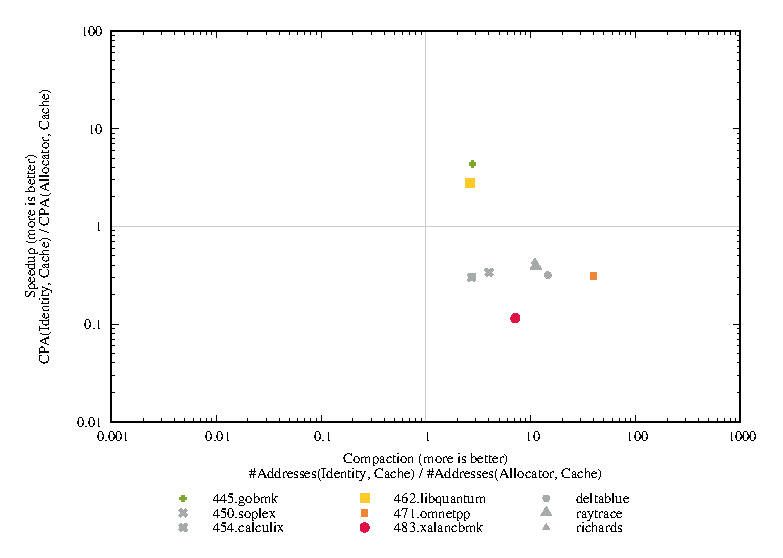
\includegraphics[width=\textwidth]{figs/plots/correlation-LRU-CompactStack.eps}
    \caption{CompactStack}
    \label{fig:correlation-lru-compactstack}
  \end{subfigure}%
  \begin{subfigure}[b]{0.5\textwidth}%
    \includegraphics[width=\textwidth]{figs/plots/correlation-LRU-CompactSet.eps}
    \caption{CompactSet}
    \label{fig:correlation-lru-compactset}
  \end{subfigure}%
  \qquad
  \begin{subfigure}[b]{0.5\textwidth}%
    \includegraphics[width=\textwidth]{figs/plots/correlation-LRU-CompactQueue.eps}
    \caption{CompactQueue}
    \label{fig:correlation-lru-compactqueue}
  \end{subfigure}%
  \begin{subfigure}[b]{0.5\textwidth}%
    \includegraphics[width=\textwidth]{figs/plots/correlation-LRU-SingleAssignment.eps}
    \caption{SingleAssignment}
    \label{fig:correlation-lru-singleassignment}
  \end{subfigure}%
  \caption{Correlation of Speedup and Compaction: LRU}
  \label{fig:correlation-lru}
\end{figure}

\Cref{fig:correlation-lru} illustrates the results of all benchmark and allocator combinations applied on the \ac{LRU} cache. Obviously, the algorithm to decided on an eviction candidate has an enormous influence.

\Cref{fig:correlation-lru-compactstack} presents the results of the CompactStack allocator in combination with the \ac{LRU} cache for all benchmarks. This figure present a quite different result an shown by \Cref{fig:correlation-min-compactstack}. In an overall view the speedup is much worse for most of the benchmark in comparison to the \ac{MIN} caches. Nevertheless, there are still three outstanding benchmarks to discuss. (1) The 471.omnetpp benchmark remains the benchmark with the most compaction. (2) The 483.xalancbmk benchmark presents the most decrease in performance. For the \ac{MIN} caches this benchmark already shows a poor speedup, but with the \ac{LRU} cache it becomes the benchmark with the least speedup. (3) The 445.gobmk benchmark and the 462.libquantum benchmark. As for the \ac{MIN} caches the 445.gobmk benchmark remains the benchmark with the most speedup. Furthermore, the 462.libquantum benchmark shows a significant improvement in speedup with the \ac{LRU} cache.

\Cref{fig:correlation-lru-compactset} presents the results of the CompactSet allocator in combination with the \ac{LRU} cache for all benchmarks. In an overall perspective also the CompactSet allocator is not able to achieve that much speedup using the \ac{LRU} cache than a \ac{MIN} cache. Most of the benchmarks present a weakening in performance which results in less speedup. Nevertheless, two benchmarks present a speedup larger than one 445.gobmk and 462.libquantum, namely. The 485.xalancbmk presents again the least speedup of all benchmarks and the 471.omnetpp remains the benchmark with most compaction.

\Cref{fig:correlation-lru-compactqueue} presents the results of the CompactQueue allocator in combination with the \ac{LRU} cache for all benchmarks. The CompactQueue allocator presents a similar behavior as the CompactStack and CompactSet allocators. Most of the data points show a weakening in speedup. The CompactQueue allocator has in an overall perspective the worst speedup results of all four allocators. In detail there are two quite interesting things to observe. First the 445.gobmk for the first time shows a speedup less than one. While 462.libquantum remains the only benchmark with a speedup greater than one. Second 483.xalancbmk is for this allocator not the benchmark with the worst speedup. The benchmark with the worst speedup is the richards benchmark.

\Cref{fig:correlation-lru-singleassignment} presents the results of the SingleAssignment allocator in combination with the \ac{LRU} cache for all benchmarks. As expected the results of the SingleAssignment allocator occur in the left lower corner. In comparison to the \ac{MIN}+Liveness cache the speedups vary more. Unexpectedly the 445.gobmk presents a speedup greater than one for the first time for this allocator.

\begin{figure}[!ht]
  \begin{subfigure}[b]{0.5\textwidth}%
    \includegraphics[width=\textwidth]{figs/plots/correlation-LRU+Liveness-CompactStack.eps}
    \caption{CompactStack}
    \label{fig:correlation-lru-liveness-compactstack}
  \end{subfigure}%
  \begin{subfigure}[b]{0.5\textwidth}%
    \includegraphics[width=\textwidth]{figs/plots/correlation-LRU+Liveness-CompactSet.eps}
    \caption{CompactSet}
    \label{fig:correlation-lru-liveness-compactset}
  \end{subfigure}%
  \qquad
  \begin{subfigure}[b]{0.5\textwidth}%
    \includegraphics[width=\textwidth]{figs/plots/correlation-LRU+Liveness-CompactQueue.eps}
    \caption{CompactQueue}
    \label{fig:correlation-lru-liveness-compactqueue}
  \end{subfigure}%
  \begin{subfigure}[b]{0.5\textwidth}%
    \includegraphics[width=\textwidth]{figs/plots/correlation-LRU+Liveness-SingleAssignment.eps}
    \caption{SingleAssignment}
    \label{fig:correlation-lru-liveness-singleassignment}
  \end{subfigure}%
  \caption{Correlation of Speedup and Compaction: LRU+Liveness}
  \label{fig:correlation-lru-liveness}
\end{figure}

\Cref{fig:correlation-lru-liveness} illustrates the results of all benchmark and allocator combinations applied on the \ac{LRU}+Liveness cache.

\Cref{fig:correlation-lru-liveness-compactstack} presents the results of the CompactStack allocator in combination with the \ac{LRU}+Liveness cache for all benchmarks. The presented speedup results are quite similar to those of the \ac{LRU} cache without liveness information. Nevertheless, one thing is still worth mentioning the 462.libquantum significantly improves its speedup. It reaches a speedup close 445.gobmk benchmark.

\Cref{fig:correlation-lru-liveness-compactset} presents the results of the CompactSet allocator in combination with the \ac{LRU}+Liveness cache for all benchmarks. The CompactSet allocators show as the CompactStack allocator only minimal improvements. Except of the 462.libquantum benchmark which improves its speedup significantly. All other benchmarks remain as before within the right left corner. This indicates a good compaction and a poor speedup.

\Cref{fig:correlation-lru-liveness-compactqueue} presents the results of the CompactQueue allocator in combination with the \ac{LRU}+Liveness cache for all benchmarks. For the CompactQueue allocator in combination with the \ac{LRU} algorithm as base of the eviction policy is seams that the liveness information has no significant influence.

\Cref{fig:correlation-lru-liveness-singleassignment} presents the results of the SingleAssignment allocator in combination with the \ac{LRU}+Liveness cache for all benchmarks. Similar to the CompactQueue allocator also for the SingleAssignment allocator is seams that the liveness information does not improve the speedup significantly.

\subsection{445.gobmk}

In this section we take a closer look at the speedup and compaction of the 445.gobmk benchmark. \Cref{fig:speedup-compaction-445-gobmk-speedup} presents an overview of the speedup results of the 445.gobmk benchmark of all allocators and caches applied.

A speedup below indicates that the performance of this allocator is worse than the performance of the Identity allocator by using the same cache. In case of the 445.gobmk there are 4 such scenarios in which an allocator performance worse than the Identity allocator.

For the \ac{MIN} cache the SingleAssignment allocators presents a speedup of $0.71$ which means that its performance is 29\% slower in comparison to the Identity allocator. For the \ac{MIN}+Liveness allocator also the SingleAssignment allocator performance worst. As expected the usage of the liveness information yields an improvement, the performance decreases by 14\%. Since the SingleAssignment allocator uses many more variables than the other allocators its results are not surprising.

For the more realistic cache implementations based on the \ac{LRU} algorithm the SingleAssignment allocator performs better and present a speedup above one. Nevertheless, there is another allocator which does not perform well on the \ac{LRU} caches, the CompactQueue. The CompactQueue allocator shows a speedup of $0.29$ for the \ac{LRU} cache and $0.34$ for the \ac{LRU} cache using liveness information. Again the liveness information has a significant influence. Nevertheless, the performance of the CompactQueue allocator is 64\%-71\% worse than the performance of the Identity allocator.

However, the CompactStack allocator is for each cache the allocator with the highest speedup. The most impressive speedup is shown for the \ac{LRU} cache, in this scenario the CompactStack allocator reaches a speedup of $4.37$. Also the CompactSet allocator presents good results overall caches.

The compaction shown by \Cref{fig:speedup-compaction-445-gobmk-compaction} is for all compacting allocators identical, which is as expecting according to the workflow presented by \Cref{fig:cache-behavior-liveness}. Its worth mentioning that all three compacting allocators are able to use $2.78$ times less variables than the Identity allocator does. Furthermore, it is not surprising that the SingleAssignment allocators requires that many more variables than the Identity allocator.

\begin{figure}[!ht]
  \centering
  \begin{subfigure}[b]{0.5\textwidth}%
    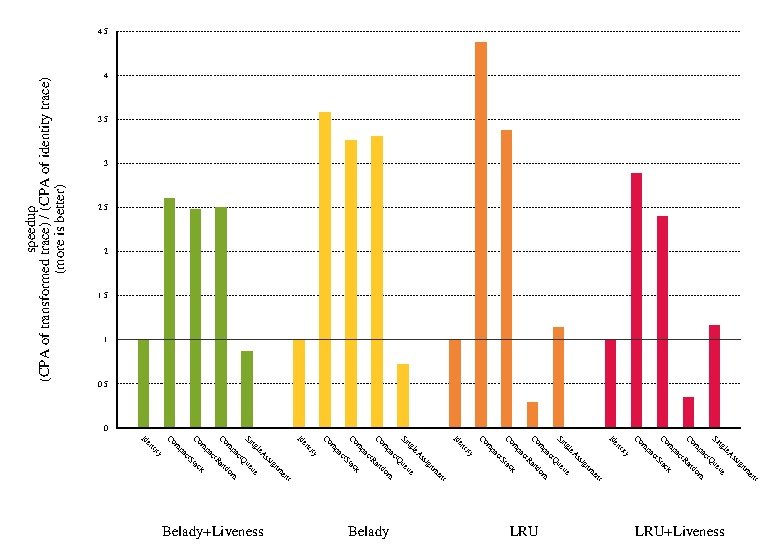
\includegraphics[width=\textwidth]{figs/plots/speedup-445-gobmk.eps}
    \subcaption{Speedup}
  \label{fig:speedup-compaction-445-gobmk-speedup}
  \end{subfigure}%
    \begin{subfigure}[b]{0.5\textwidth}%
    \includegraphics[width=\textwidth]{figs/plots/compaction-445-gobmk.eps}
    \subcaption{Compaction}
  \label{fig:speedup-compaction-445-gobmk-compaction}
  \end{subfigure}%
  \caption{Speedup \& Compaction: 445.gobmk}
  \label{fig:speedup-compaction-445-gobmk}
\end{figure}

\subsection{471.omnetpp}

\Cref{fig:speedup-compaction-471-omnetpp} presents the results of the 471.omnetpp benchmark in detail.

\Cref{fig:speedup-compaction-471-omnetpp-speedup} shows the speedup of all allocators and caches of the 471.omnetpp benchmark. Obviously, the speedup results of the 471.omnetpp benchmark are significant worse than those of the 445.gobmk benchmark. Just for the two caches \ac{MIN} and \ac{MIN}+Liveness the 471.omnetpp benchmark is able to achieve a speedup greater than one at all. And for these caches only the compacting allocators are slightly greater than one. The results for the \ac{LRU} caches are dramatically worse. For the \ac{LRU} caches non of the allocators is able to achieve a speedup close to one. However, the CompactionStack allocator presents the best results o all allocators and again the CompactQueue allocators shows the worst results.

\Cref{fig:speedup-compaction-471-omnetpp-compaction} presents the compaction of the 471.omnetpp benchmark. As the previous figures suggested the compaction of the 471.omnetpp benchmark is extremely high. All compacting allocators require $39.76$ times less variables than the Identity allocator does. Furthermore, the compaction of the SingleAssignment allocator is quite interesting, because it indicates that the \ac{trace} consists of many store instructions which lead to a compaction of $0.004$.

\begin{figure}[!ht]
  \begin{subfigure}[b]{0.5\textwidth}%
    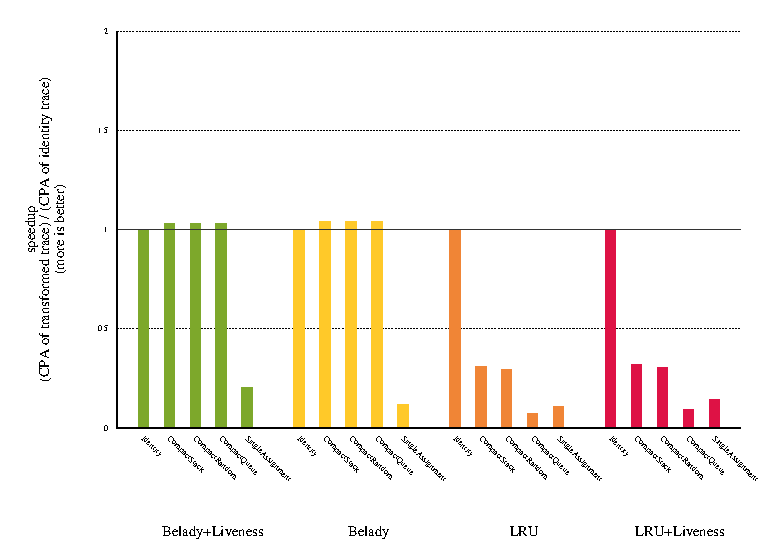
\includegraphics[width=\textwidth]{figs/plots/speedup-471-omnetpp.eps}
    \subcaption{Speedup}
    \label{fig:speedup-compaction-471-omnetpp-speedup}
  \end{subfigure}%
  \begin{subfigure}[b]{0.5\textwidth}%
    \includegraphics[width=\textwidth]{figs/plots/compaction-471-omnetpp.eps}
    \subcaption{Compaction}
    \label{fig:speedup-compaction-471-omnetpp-compaction}
  \end{subfigure}%
  \caption{Speedup \& Compaction: 471.omnetpp}
  \label{fig:speedup-compaction-471-omnetpp}
\end{figure}

\subsection{483.xalancbmk}

\Cref{fig:speedup-compaction-483-xalancbmk} presents the results of the 483.xalancbmk benchmark in detail.

\Cref{fig:speedup-compaction-483-xalancbmk-speedup} shows the speedup results of the 483.xalancbmk. Unfortunately, the presented results show only two scenarios for which a speedup greater than one can be achieved. Namely, this scenarios are the CompactStack allocator in combination with the \ac{MIN} cache and the CompactStack allocator in combination with the \ac{MIN}+Liveness cache. The CompactSet allocator is close to one but stays below even if a cache uses the liveness information. On the \ac{LRU} caches non of the presented allocators is able to achieve a speedup above $0.15$. Which means that all allocators show a performance at least 85\% worse than the Identity allocators performance.

However, \Cref{fig:speedup-compaction-483-xalancbmk-compaction} presents quite good results for the compaction. The compacting allocators are able to use $7.14$ times less variables than the Identity allocators does.

\begin{figure}[!ht]
  \begin{subfigure}[b]{0.5\textwidth}%
    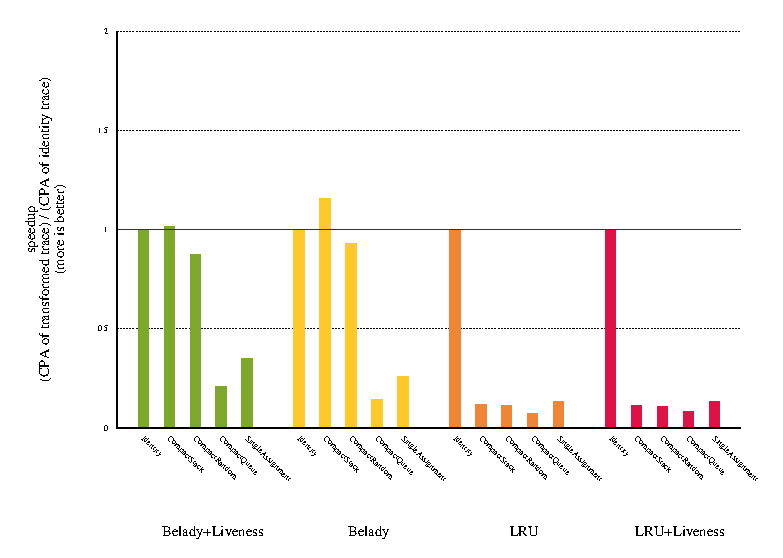
\includegraphics[width=\textwidth]{figs/plots/speedup-483-xalancbmk.eps}
    \subcaption{Speedup}
    \label{fig:speedup-compaction-483-xalancbmk-speedup}
  \end{subfigure}%
  \begin{subfigure}[b]{0.5\textwidth}%
    \includegraphics[width=\textwidth]{figs/plots/compaction-483-xalancbmk.eps}
    \subcaption{Compaction}
    \label{fig:speedup-compaction-483-xalancbmk-compaction}
  \end{subfigure}%
  \caption{Speedup \& Compaction: 483.xalancbmk}
  \label{fig:speedup-compaction-483-xalancbmk}
\end{figure}

\section{Performance}\label{sec:experiment-performance}

This section presents the performance of the benchmarks. The performance is computed as explained by \Cref{sec:performance}. All figures of this section show the \ac{CPA} on the y-axis, computed as illustrated by \Cref{equ:performance-cpa}, on the x-axis the allocators are shown in groups of the applied cache. Additional to the performance we take a look at the distribution of cache misses and caches hits and influences of the different kinds of memory accesses. By now we focus on the benchmarks, \emph{445.gobmk}, \emph{471.omnetpp}, and \emph{483.xalancbmk}, namely. The remaining figures can be found at \Cref{app:experiment}. For each benchmark two figures are presented. Both figures show the performance in \ac{CPA}, but the figure on the left hand-side additionally presents the distribution of cache misses and cache hits and the figure on the right hand-side illustrates the different kinds of memory accesses.

\subsection{445.gobmk}
\Cref{fig:performance-445-gobmk} presents the results of the 445.gobmk benchmark. For each group of allocators, e.g., the five allocators Identity, CompactStack, CompactSet, CompactQueue, and SingleAssignment of the \ac{LRU} group, the results of Identity represent the baseline. Lets stick with the first group the baseline is a CPA of $15.22$. The allocators CompactStack, CompactSet, and SingleAssignment perform better than the Identity. This means the performance of the original \ac{trace} offers potential of improvement, as shown by these three allocators. However, not all of them show an improvement. The CompactQueue allocators presents a dramatically worse performance than Identity. Nevertheless, we observe that the \ac{CPA} of the CompactQueue presented by the \ac{LRU} cache is the worst. For the other cache implementation its performance is significant better. In more detail the CompactQueue performs much better on the MIN caches than on the \ac{LRU} caches. For the MIN caches the performance of the SingleAssignment approach is the worst. For completeness the CompactStack performance best on all cache implementations. This nicely illustrates the influence of the underlining cache. It seams that all allocators benefit from the usage of liveness information. Not surprisingly the MIN cache is beatifically for all allocators.
Taking in account the shown cache misses and cache hits the poor performance of the CompactQueue is not that surprising anymore. Obviously, the CompactQueue implementation yields the most cache misses, e.g., for the \ac{LRU} cache. Which in this case leads to more main memory accesses as illustrated by \Cref{fig:performance-445-gobmk-memops}. For all other allocators there much less main memory loads and main memory stores.
Summarizing the \Cref{fig:performance-445-gobmk} illustrate that there is potential for performance improvement of the 445.gobmk benchmark. Furthermore, the presents of differences between the cache implementations is shown.

\begin{figure}[!ht]
  \begin{subfigure}[b]{0.5\textwidth}%
    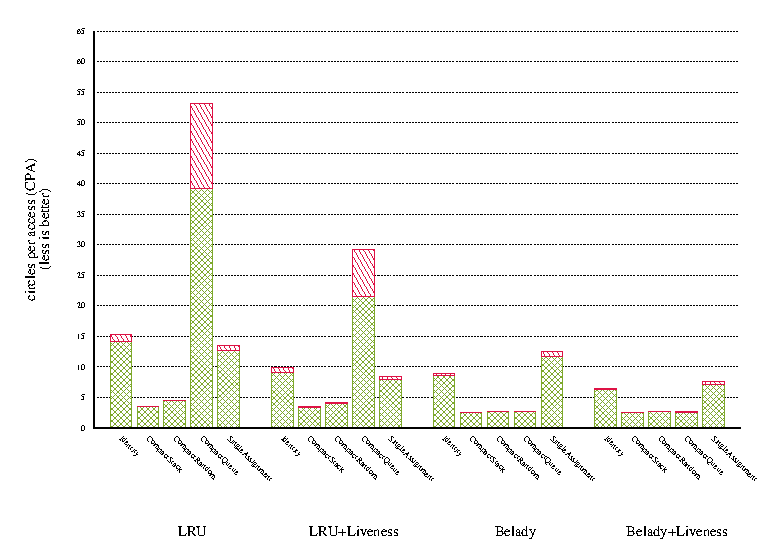
\includegraphics[width=\textwidth]{figs/plots/perf-misses-445-gobmk.eps}
    \subcaption{Cache misses and cache hits}
    \label{fig:performance-445-gobmk-misses}
  \end{subfigure}%
  \begin{subfigure}[b]{0.5\textwidth}%
    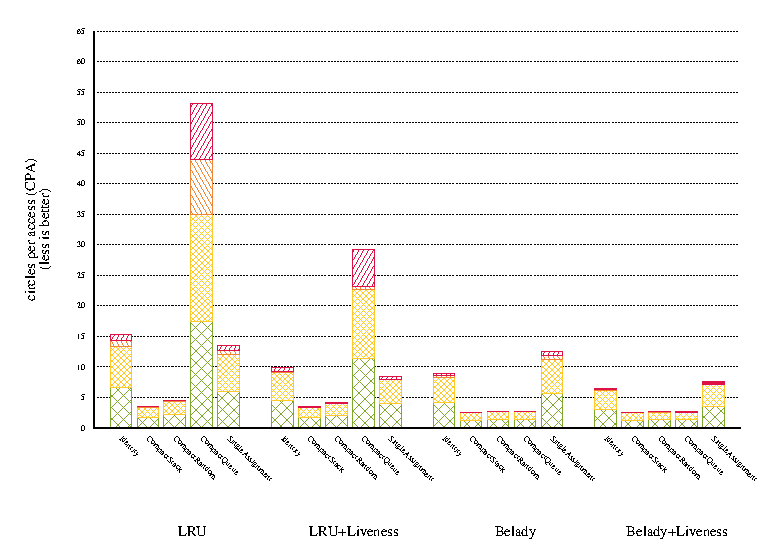
\includegraphics[width=\textwidth]{figs/plots/perf-445-gobmk.eps}
    \subcaption{Types of memory operations}
    \label{fig:performance-445-gobmk-memops}
  \end{subfigure}%
  \caption{Performance: 445.gobmk}
  \label{fig:performance-445-gobmk}
\end{figure}

\subsection{471.omnetpp}
\Cref{fig:performance-471-omnetpp} presents the performance results of the 471.omnetpp benchmark. As before both figures illustrate the performance in \ac{CPU}, but on the left hand-side the distribution of cache misses and cache hits is shown and on th right hand-side the relation of the different memory accesses is presented. For this benchmark the Identity results are much better than results of the 445.gobmk. Since the Identity \ac{CPA}s are quite close to 1 ($1.85$, $1.82$, $1.04$, and $1.03$) there is not much space for improvement, especially for the \ac{MIN} implementations. Nevertheless, only for the \ac{MIN} implementation we are able to achieve an improvement with the allocators CompactStack, CompactSet, and CompactQueue. The approach without compaction, SingleAssignment, seams to be a bad chose for this benchmark, for all four cache implementations it shows poor performance. As before it is observable that those allocators with less cache misses end up with less main memory accesses. What is plausible although a cache miss does not necessarily force a main memory access, as \Cref{fig:cache-behavior-liveness} illustrates. According to the work flow shown by \Cref{fig:cache-behavior-liveness} the hypothesis raises that the 471.omnetpp benchmark consists of many variables with overlapping liveness intervals or this benchmark is very load intensive or both aspects are more pronounced compared to 445.gobmk.


\begin{figure}[!ht]
  \begin{subfigure}[b]{0.5\textwidth}%
    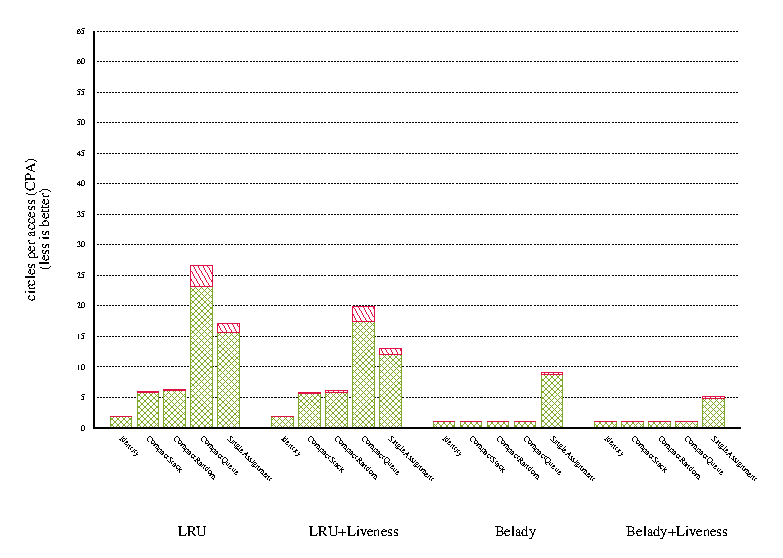
\includegraphics[width=\textwidth]{figs/plots/perf-misses-471-omnetpp.eps}
    \subcaption{Cache misses and cache hits}
    \label{fig:performance-471-omnetpp-misses}
  \end{subfigure}%
  \begin{subfigure}[b]{0.5\textwidth}%
    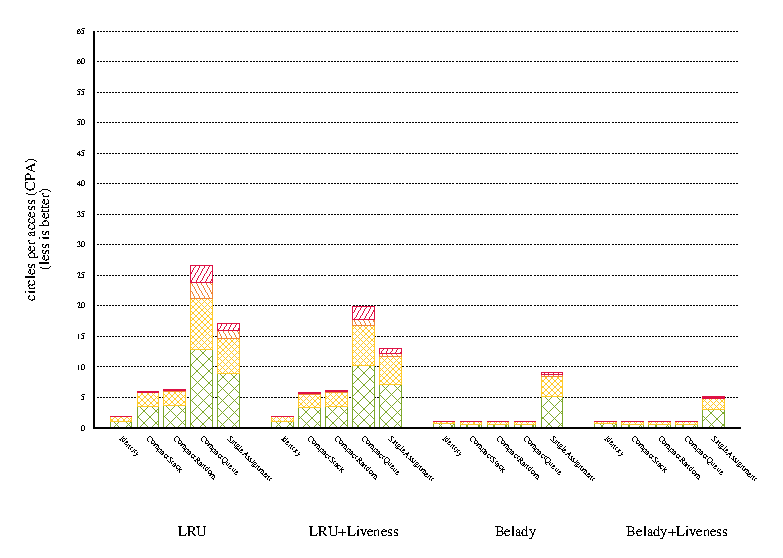
\includegraphics[width=\textwidth]{figs/plots/perf-471-omnetpp.eps}
    \subcaption{Types of memory operations}
    \label{fig:performance-471-omnetpp-memops}
  \end{subfigure}%
  \caption{Performance: 471.omnetpp}
  \label{fig:performance-471-omnetpp}
\end{figure}

\subsection{483.xalancbmk}
\Cref{fig:performance-483-xalancbmk} illustrates the performance of the 483.xalancbmk. The most obvious observation is that the performance gap of the \ac{LRU} cache implementations and the \ac{MIN} implementations is dramatical. Hence, the \ac{LRU} cache is not the optimal cache for our compacting allocators. In a worst case our transformations yield approximately a 10 times worse \ac{CPA} than the Identity. The source of this poor performance seams to be that the compaction increases the number of cache misses. Unfortunately, many of the cache misses yield a main memory access, as illustrated by \Cref{fig:performance-483-xalancbmk-memops}. Peeking CompactQueue as out standing example the number of cache misses is nearly identical with the number of main memory access which leads to its poor performance. As expected the implementation of the \ac{LRU} cache which uses the liveness information is able a better \ac{CPA} for all allocators. But even those results are far from good. However, the results for the \ac{MIN} caches are much better than those of the \ac{LRU} caches. Even though the performance of the \ac{MIN} caches is much better there is only one allocator which is able to improve the performance in comparison to the Identity allocator, CompactStack namely. CompactSet is close to the original performance but the other tow CompactQueue, and SingleAssignment do not perform as well.

\begin{figure}[!ht]
  \begin{subfigure}[b]{0.5\textwidth}%
    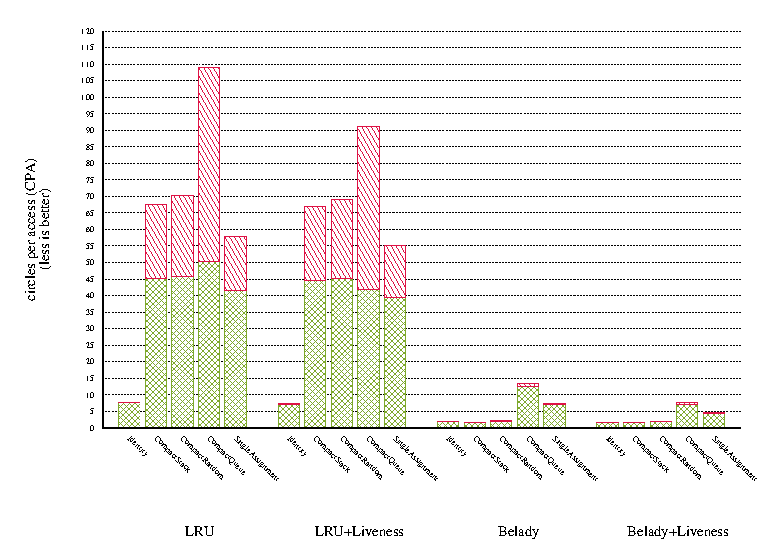
\includegraphics[width=\textwidth]{figs/plots/perf-misses-483-xalancbmk.eps}
    \subcaption{Cache misses and cache hits}
    \label{fig:performance-483-xalancbmk-misses}
  \end{subfigure}%
  \begin{subfigure}[b]{0.5\textwidth}%
    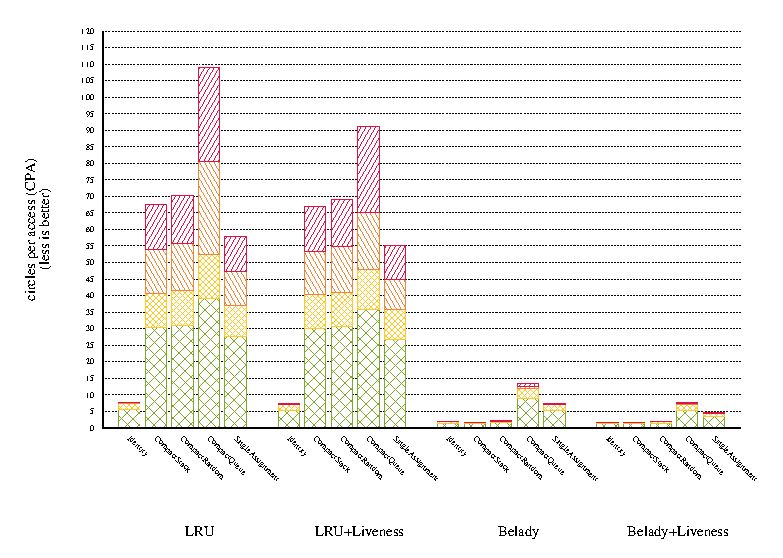
\includegraphics[width=\textwidth]{figs/plots/perf-483-xalancbmk.eps}
    \subcaption{Types of memory operations}
    \label{fig:performance-483-xalancbmk-memops}
  \end{subfigure}%
  \caption{Performance: 483.xalancbmk}
  \label{fig:performance-483-xalancbmk}
\end{figure}

\section{Statistical Analysis}
\label{sec:experiment-statistical-analysis}

This section presents the statistical analysis on the benchmarks according to the metrics presented in \Cref{sec:metrics}. The metrics presented are observed from the Identity allocator. More details and further tables can be found in \Cref{app:experiment}.

\begin{table}[!ht]
  \centering
  \begin{tabular}[c]{lrrrr}
    \hline
    Benchmark & Size [MB] & Number of Instructions & Loads [\%] & Stores [\%] \tabularnewline
    \hline
    445.gobmk      & 1781.76 &  \num{186740466} & 50.20 & 49.80 \tabularnewline
    450.soplex     &  196.29 &   \num{20582523} & 27.90 & 72.10 \tabularnewline
    454.calculix   &  505.71 &   \num{53027458} & 31.93 & 68.07 \tabularnewline
    462.libquantum &  945.71 &   \num{99165026} & 14.28 & 85.72 \tabularnewline
    741.omnetpp    & 8069.12 & \num{8459396786} & 39.40 & 60.60 \tabularnewline
    483.xalancbmk  & 1269.76 &  \num{133660557} & 25.47 & 74.53 \tabularnewline
    richards       &  790.51 &   \num{82890768} & 24.90 & 75.10 \tabularnewline
    raytrace       &  591.43 &   \num{62015988} & 35.33 & 64.67 \tabularnewline
    deltablue      & 2590.72 &  \num{272165756} & 25.62 & 74.38 \tabularnewline
    \hline
  \end{tabular}
  \caption{Basic benchmark data}
  \label{tab:basic-benchmark-data}
\end{table}

\Cref{tab:basic-benchmark-data} shows the most basic data for all benchmarks analyzed. According to the size of a benchmark the number of instructions varies. The column \emph{Number of Instructions} shows the total number of load and store instructions. The columns \emph{Loads} and \emph{Store} present the distribution of loads and stores in percentage. Most of the listed benchmarks are store-intensive, consists of more store instructions than load instructions. Except the 445.gobmk benchmark that presents a distribution of $50.20$ percent loads and $49.8$ percent stores. 462.libquantum consists of $85.72$ percent stores which is the maximum for all benchmarks listed.

\begin{table}[!ht]
  \centering
  \begin{tabular}{lrrr}
    \hline
     & 445.gobmk & 471.omnetpp & 483.xalancbmk\\
    \hline
    \csvreader[late after line=\\]{figs/statistical-analysis-data/prepared-address-accesses-3.csv}%
    {1=\collabel, 2=\colgobmk, 3=\colomnetpp, 4=\colxalancbmk}%
    {\collabel & \num{\colgobmk} & \num{\colomnetpp} & \num{\colxalancbmk}}%
    \hline
  \end{tabular}
  \caption{Metric: Accesses}
  \label{tab:metric-accesses-3}
\end{table}

\Cref{tab:metric-accesses-3} presents the results about the access distance for the benchmarks 445.gobmk, 471.omnetpp, and 483.xalancbmk. \Cref{tab:metric-accesses-all} presents the results for all benchmarks. \emph{Count} represents the number of different variables used. The arithmetic mean shows that a variables of 445.gobmk are accessed $111.56$ times in average, variables of 471.omnetpp are accessed $859.89$ times in average, and variable of 483.xalancbmk are accessed $155.57$ times in average. Clearly the variables of the 471.omnetpp benchmarks are accessed most in average. \emph{Minimum} and \emph{maximum} show that there exists at least one variable that is accessed only once and that there is at least on variable with is accessed $12057070$, $19444797$, and $2416458$ for the benchmarks 445.gobmk, 471.omnetpp, and 483.xalancbmk. Investigating the results of the percentiles shows that the \emph{average} is misleading. For the 445.gobmk the 95\% percentile presents a value of $23$. Hence, 95\% of all variables are accessed at most 23 times. This indicates that the remaining 5\% of the variables are accessed significantly more often. Otherwise the \emph{average} would not result in a value that high. These values indicate that half of the variables are accessed with high frequency. The 25\% percentile shows that there variables which are accessed with even higher frequency. The 445.gobmk benchmark presents a 25\% percentile of $3$. On the opposite the results of the 445.gobmk benchmark for the 95\% percentile illustrate that 5\% of the variables used are accessed with large distances, a low frequency. For the benchmarks 471.omnetpp and 483.xalancbmk the 95\% percentile is significantly larger then the 75\% percentile that show the same behavior as for the 445.gobmk benchmark. However, the increase is significantly less than for the 445.gobmk. The 471.omnetpp benchmark presents a similar behavior as the 445.gobmk benchmark. The most significant difference is that the variable are in general accessed more often, this is observable for example from the 50\% percentile. The 483.xalancbmk shows a significant gap between 75\% percentile and 95\% percentile. Indicating that 25\% of the used variables are accessed significantly more often that the others.

\begin{table}[!ht]
  \centering
  \begin{tabular}{lrrr}
    \hline
     & 445.gobmk & 471.omnetpp & 483.xalancbmk\\
    \hline
    \csvreader[late after line=\\]{figs/statistical-analysis-data/prepared-access-distances-3.csv}%
    {1=\collabel, 2=\colgobmk, 3=\colomnetpp, 4=\colxalancbmk}%
    {\collabel & \num{\colgobmk} & \num{\colomnetpp} & \num{\colxalancbmk}}%
    \hline
  \end{tabular}
  \caption{Metric: Access Distance}
  \label{tab:metric-access-distance-3}
\end{table}

\Cref{tab:metric-access-distance-3} presents the results about the access distance for the benchmarks 445.gobmk, 471.omnetpp, and 483.xalancbmk. \Cref{tab:metric-access-distance-all} presents the results for all benchmarks. \emph{Count} represents the number of different access distances observed for a benchmark. This table shows a large gap between \emph{minimum} and \emph{maximum} access distance. The table show that the \emph{minimum} is $1$ for all benchmarks that indicates that at least one variable is accessed twice without accessing another variable in between. The \emph{maximum} indicates for all three benchmarks that there is at least one variable with is accessed rarely. The \emph{average} access distance is significantly smaller than the \emph{maximum}. The percentiles offer a deeper knowledge about the actual access distances. The $50$\% percentile is identical to the \emph{median}. It shows for the 445.gobmk benchmark that $50$\% of the used variables have an access distance of less equal to $73$. That is several magnitudes less than the average. For the other two benchmarks the situation is similar, 471.omnetpp presents an 50\% percentile of $41$ and the 483.xalancbmk show a value of $394$.

\begin{table}[!ht]
  \centering
  \begin{tabular}{lrrr}
    \hline
     & 445.gobmk & 471.omnetpp & 483.xalancbmk\\
    \hline
    \csvreader[late after line=\\]{figs/statistical-analysis-data/prepared-live-addresses-3.csv}%
    {1=\collabel, 2=\colgobmk, 3=\colomnetpp, 4=\colxalancbmk}%
    {\collabel & \num{\colgobmk} & \num{\colomnetpp} & \num{\colxalancbmk}}%
    \hline
  \end{tabular}
  \caption{Metric: Overlapping Liveness}
  \label{tab:metric-overlapping-liveness-3}
\end{table}

\Cref{tab:metric-overlapping-liveness-3} presents the results about the access distance for the benchmarks 445.gobmk, 471.omnetpp, and 483.xalancbmk. \Cref{tab:metric-overlapping-liveness-all} presents the results for all benchmarks. \emph{Count} represents the number of overlapping liveness intervals. The table shows that for the 445.gobmk benchmark at least $67$ variables are live at the same time,  $83$ at the 471.omnetpp, and $75$ at the 283.xalancbmk. The 5\% percentile for all three benchmarks shows that during execution there are significantly more variables live at the same time. This indicates that the working set of these three benchmarks definitely does not fit into the cache for this experiment.

\begin{table}[!ht]
  \centering
  \begin{tabular}{lrrr}
    \hline
     & 445.gobmk & 471.omnetpp & 483.xalancbmk\\
    \hline
    \csvreader[late after line=\\]{figs/statistical-analysis-data/prepared-liveness-length-3.csv}%
    {1=\collabel, 2=\colgobmk, 3=\colomnetpp, 4=\colxalancbmk}%
    {\collabel & \num{\colgobmk} & \num{\colomnetpp} & \num{\colxalancbmk}}%
    \hline
  \end{tabular}
  \caption{Metric: Liveness Interval Length}
  \label{tab:metric-liveness-length-3}
\end{table}

\Cref{tab:metric-liveness-length-3} presents the results about the access distance for the benchmarks 445.gobmk, 471.omnetpp, and 483.xalancbmk. \Cref{tab:metric-liveness-interval-length-all} presents the results for all benchmarks. \emph{Count} represents the number of different liveness interval lengths. The results of the 445.gobmk benchmark indicate that most variables have short liveness intervals. This is indicated by the percentiles 5\%, 25\%, 50\%, and 75\%, which all present value $0$. In this context $0$ means that a variable is live for exactly one access. Hence, 75\% of the variables of the 445.gobmk benchmark are accessed only once. By the delta of the 75\% percentile and 95\% percentile we know that 20\% percent of the used variables are have a liveness interval of a length up to $156$. In combination with the fact that all variables used accumulate to an average liveness interval length of $1402011.75$, this implies that 5\% of the variables used by 445.gobmk consists of a significantly longer liveness interval. The results of the 471.omnetpp benchmark and the 483.xalancbmk benchmark indicate that there is a small amount of variables that significantly longer than the majority of the used variables.

\Cref{fig:stats-overview} presents the results of all statistical metrics of all benchmarks. Note that the y-axis is logarithmic and the x-axis is linear.

\Cref{fig:stats-liveness-interval-length} presents the liveness interval lengths on the y-axis. On the x-axis the liveness interval lengths of all variables are shown in decreasingly sorted.
% 445.gobmk
As illustrated by \Cref{fig:stats-liveness-interval-length} over 90\% of the liveness intervals of the 445.gobmk are of length 1 and less than 5\% are of a length longer than 5.
% 462.libquantum
Approximately 20\% of the liveness intervals of the 462.libquantum benchmark are of length greater equal 5, less than 10\% are or length greater equal 100, and over 65\% of the liveness intervals are of length 1.
% 471.omnetpp
The 471.omnetpp benchmarks consists of approximately 5\% of liveness intervals with a length greater 100, slightly more than 10\% are of a length great than 1, and slightly less than 90\% of the liveness intervals are of length 1.
% 483.xalancbmk
Approximately 20\% of the liveness intervals of the 483.xalancbmk benchmark are of a length greater than 1 and approximately 5\% of the liveness intervals are of a length greater than 2

\Cref{fig:stats-overlapping-liveness} shows the number of overlapping liveness intervals on the y-axis.
% 445.gobmk
The 445.gobmk benchmark presents the most overlapping liveness intervals. Different to the other benchmarks the number of overlapping liveness interval do net reduce exactly line, there are several steps observable.
% 462.libquantum
The 462.libquantum benchmark is one of the benchmarks with the fewest overlapping liveness intervals. Then number of liveness intervals reduces linear.
% 471.omnetpp
The 471.omnetpp benchmark consists of significant more overlapping liveness intervals than all other benchmarks except the 445.gobmk benchmark. In difference to the 445.gobmk benchmark the number of overlapping liveness intervals of the 471.omnetpp benchmark decreases linear.
% 483.xalancbmk
The 483.xalancbmk benchmark is one of the benchmarks with the fewest overlapping liveness intervals. The number of overlapping liveness intervals decreases linear.

\Cref{fig:stats-accesses} shows the number of access at a variable on the y-axis.
On the x-axis the values of all variables are shown in decreasing order.
% 445.gobmk
Approximately 5\% of the variables of the 445.gobmk benchmark are accesses more often than 20 times, almost 3\% are accessed less than 20 times, and the remaining $\sim$92\% of the variables are accessed exactly 20 times.
% 462.libquantum
For the 462.libquantum benchmark approximately 35\% of the variables are accessed once, $\sim$15\% are accessed 2 times, almost 40\% of the variables are accessed more often than 2 times and less often than 200 times, and less than 10\% are accessed over 200 times.
% 471.omnetpp
10\% of the 471.omnetpp benchmarks variables are accessed less than 20 times, approximately 85\% are of the variables are accessed between 20 and 400 times, and the remaining around 5\% of the variables are accessed over 400 times.
% 483.xalancbmk
Almost 45\% of the variables of the 483.xalancbmk benchmark are accessed at most 10 times, approximately 30\% of the variables are accessed between 10 and 20 times, almost 15\% are accessed between 20 and 100 times, and the remaining $\sim$ 10\% are accessed more often than 100 times.

\Cref{fig:stats-access-distance} illustrates the access distances on the y-axis and on the x-axis all observed values are shown in decreasing order.
% 445.gobmk
Only approximately 35\% of the access distances of the 445.gobmk benchmark are greater than 1, less than 10\% are greater than 10, and just a few percentage of the access distances are greater than 100.
% 462.libquantum
Over 50\% of the accesses distances of the 462.libquantum benchmark are greater than 1, almost 32\% are greater than 5, less than 5\% of the access distances are greater than 100, and less than 3\% are even greater 1000.
% 471.omnetpp
Slightly less than 40\% of the access distances are greater than 1, approximately 35\% are greater than 3, and only less than 20\% are greater than 3.
% 483.xalancbmk
Less than 30\% of the access distances are greater than 1, approximately 20\% are of access distance 2, and roughly 2\% of the access distances are greater than 10.

\begin{figure}[!ht]
  \begin{subfigure}[b]{0.5\textwidth}%
    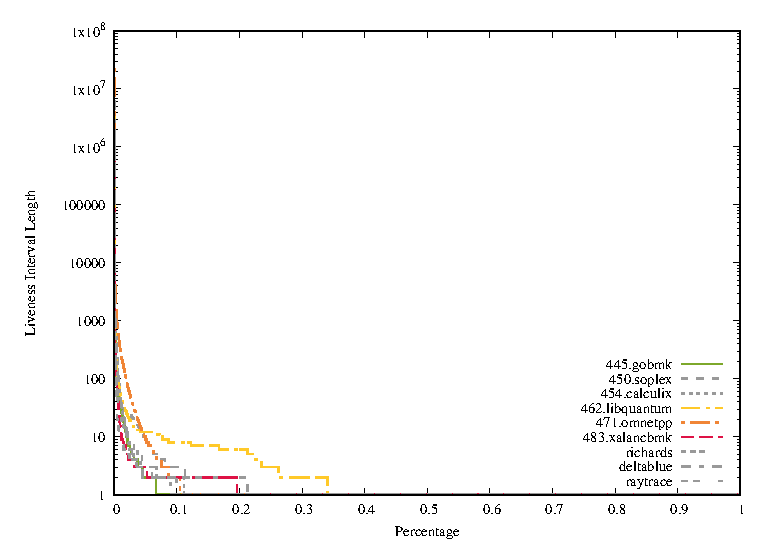
\includegraphics[width=\textwidth]{figs/statistical-analysis/plots/ll.eps}
    \subcaption{Liveness Interval Length}
    \label{fig:stats-liveness-interval-length}
  \end{subfigure}
  \begin{subfigure}[b]{0.5\textwidth}%
    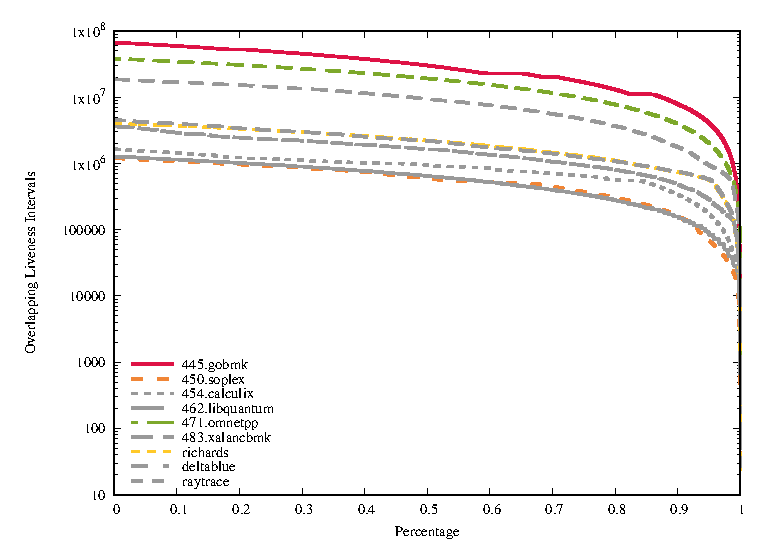
\includegraphics[width=\textwidth]{figs/statistical-analysis/plots/ol.eps}
    \subcaption{Overlapping Liveness Intervals}
    \label{fig:stats-overlapping-liveness}
  \end{subfigure}
  \begin{subfigure}[b]{0.5\textwidth}%
    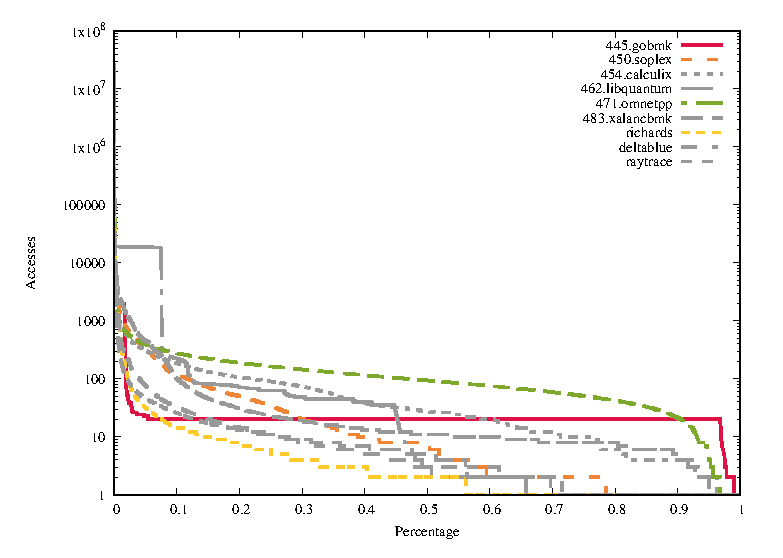
\includegraphics[width=\textwidth]{figs/statistical-analysis/plots/aa.eps}
    \subcaption{Accesses}
    \label{fig:stats-accesses}
  \end{subfigure}
  \begin{subfigure}[b]{0.5\textwidth}%
    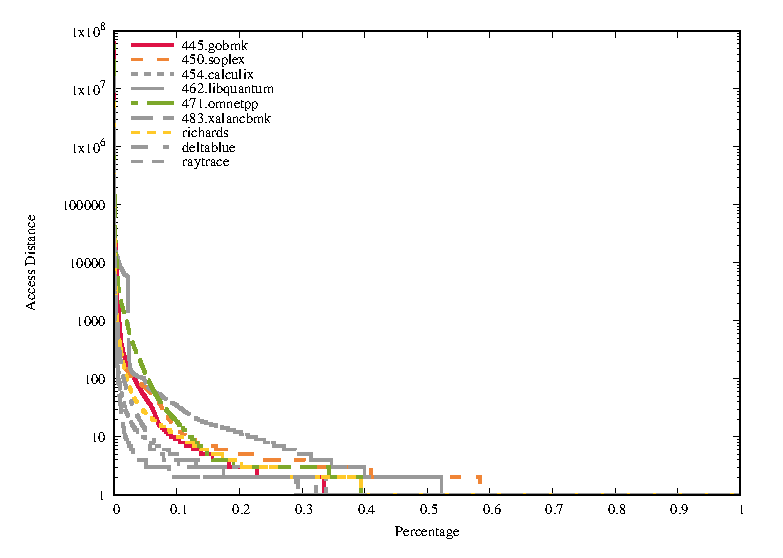
\includegraphics[width=\textwidth]{figs/statistical-analysis/plots/ad.eps}
    \subcaption{Access Distance}
    \label{fig:stats-access-distance}
  \end{subfigure}
  \caption{Statistical analysis: metrics overview}
  \label{fig:stats-overview}
\end{figure}

\section{Conclusion}\label{sec:exp-conclusion}

\Cref{cha:experiment} presents an experiment based on our environment to illustrate the difference of our cache implementations, of our allocator implementations, and the used benchmarks.
The correlation of speedup and compaction presents that there are several benchmarks that show an outstanding good results: 445.gobmk, 471.omnetpp, and 483.xalancbmk.

The 445.gobmk benchmark presents that there is potential for performance improvement by picking the appropriate allocator.
In this case CompactStack and CompactSet, namely.
Further, it also illustrates that the performance can become significantly worse than the base line performance by deciding on one of the other allocators.
For this benchmark the CompactQueue allocators presents the worst performance results.
The 445.gobmk benchmark is characterized by few accesses and extremely short liveness intervals for most of the used variables, that yields in a significant performance improvement indicated by the speedup.

The 471.omnetpp benchmark presents less potential for performance improvement.
Nevertheless, with the \ac{MIN} caches end up with quite close to the optimal \ac{CPA}.
That is quite impressive facing that small margin of improvement potential.
Unfortunately, non of our allocators is able to result in a speedup greater than one.
However, the 471.omnetpp benchmark presents a remarkable compaction.
Using one of our compacting allocators reduced the necessary memory nearly by 40 times.
The 471.omnetpp benchmark is characterized by short access distances and short liveness intervals for most of the used variables, that yields in a dramatical reduction for the memory required to execute this benchmark.

The 483.xalancbmk present a significant gap in terms of performance for the \ac{LRU} and \ac{MIN} cache implementations.
Further, the CompactStack allocator is the only implementation that is able to perform better than the original \ac{trace}.
As for the benchmarks 445.gobmk and 471.omnetpp the CompactQueue allocator presents the worst performance.
The 483.xalancbmk benchmark is characterized by few accesses and long liveness intervals for most of the used variables, that indicates that long liveness intervals are not beneficial for the performance.

In most of our experiments the results of the CompactQueue allocator have been outperformed by the CompactStack allocator, or the CompactSet allocator, or both.
Intuitively, the CompactQueue implementation picks always the variable which has been freed least recently (longest ago).
While the stack implementation of the free list enables the CompactStack to pick the most recently freed variable (shortest ago).
Obviously, the most recently freed variable has a high probability to still be in the cache than the variable least recently freed.

%%%%%%%%%%%%%%%%%%%%%%%%%%%%%%%%%%%%%%%%%%%%%%%%%%%%%%%%%%%%%%%%%%%%%%%%%%%%%%%%%%%%%%%%%%%%%%%%%%%
%%%%%%%%%%%%%%%%%%%%%%%%%%%%%%%%%%%%%%%%%%%%%%%%%%%%%%%%%%%%%%%%%%%%%%%%%%%%%%%%%%%%%%%%%%%%%%%%%%%
%%%%%%%%%%%%%%%%%%%%%%%%%%%%%%%%%%%%%%%%%%%%%%%%%%%%%%%%%%%%%%%%%%%%%%%%%%%%%%%%%%%%%%%%%%%%%%%%%%%
%%%%%%%%%%%%%%%%%%%%%%%%%%%%%%%%%%%%%%%%%%%%%%%%%%%%%%%%%%%%%%%%%%%%%%%%%%%%%%%%%%%%%%%%%%%%%%%%%%%

% \chapter{Related Work}\label{cha:related-work}
% \torevise\\

%%%%%%%%%%%%%%%%%%%%%%%%%%%%%%%%%%%%%%%%%%%%%%%%%%%%%%%%%%%%%%%%%%%%%%%%%%%%%%%%%%%%%%%%%%%%%%%%%%%
%%%%%%%%%%%%%%%%%%%%%%%%%%%%%%%%%%%%%%%%%%%%%%%%%%%%%%%%%%%%%%%%%%%%%%%%%%%%%%%%%%%%%%%%%%%%%%%%%%%
%%%%%%%%%%%%%%%%%%%%%%%%%%%%%%%%%%%%%%%%%%%%%%%%%%%%%%%%%%%%%%%%%%%%%%%%%%%%%%%%%%%%%%%%%%%%%%%%%%%
%%%%%%%%%%%%%%%%%%%%%%%%%%%%%%%%%%%%%%%%%%%%%%%%%%%%%%%%%%%%%%%%%%%%%%%%%%%%%%%%%%%%%%%%%%%%%%%%%%%

\chapter{Conclusion \& Future Work}\label{cha:conclusion}

% what we did
In this work, we have analyzed the memory access traces of nine benchmarks taken from two different benchmark suits, SPEC 2006 and V8.
We have transformed the observed traces of all benchmarks by using different allocators: Identity, CompactStack, CompactSet, CompactQueue, and SingleAssignment.
Each of the transformed traces has been executed on four different caches to observe the data about their performance and memory usage.
These four caches use two different algorithms to decide on an eviction candidate, namely \ac{LRU} and \citeauthor{belady1966study}.
For each eviction policy, there is one version that uses the liveness information of a trace and a second one that proceeds without using liveness information.
To reason about the performance and memory usage results we analyzed the observed memory access trace according to the four metrics: accesses, access distance, liveness interval length, and overlapping liveness.
% results
The presented experiments illustrate that the analyzed memory access traces have potential for improvement.
Our extremely simple allocators used for transformation reveal that each \ac{trace} uses at least twice the memory than necessary.
However, the drawback of these extremely simple allocators is shown in the performance results, most benchmarks achieve a worse performance after transformation.
The defined metrics, used to reason about performance and memory usage, illustrate tendencies for improvement rather than unique characteristics.
% conclustions
We were able to show that even modern computer programs have not reached there limits yet, there is still space for improvement.
Unfortunately, the chosen metrics are not as expressive than we have assumed.

% future work
Implementation of more sophisticated allocators that improve the quality of the trace transformations remains for future work.
Further, the set of available caches could be extended by implementing additional eviction policies.
Moreover, other benchmark suites could be integrated and analyzed.
The additional data could lead to further metrics, that may allow stronger statements or
 reveal new characteristics.

%%%%%%%%%%%%%%%%%%%%%%%%%%%%%%%%%%%%%%%%%%%%%%%%%%%%%%%%%%%%%%%%%%%%%%%%%%%%%%%%%%%%%%%%%%%%%%%%%%%
%%%%%%%%%%%%%%%%%%%%%%%%%%%%%%%%%%%%%%%%%%%%%%%%%%%%%%%%%%%%%%%%%%%%%%%%%%%%%%%%%%%%%%%%%%%%%%%%%%%
%%%%%%%%%%%%%%%%%%%%%%%%%%%%%%%%%%%%%%%%%%%%%%%%%%%%%%%%%%%%%%%%%%%%%%%%%%%%%%%%%%%%%%%%%%%%%%%%%%%
%%%%%%%%%%%%%%%%%%%%%%%%%%%%%%%%%%%%%%%%%%%%%%%%%%%%%%%%%%%%%%%%%%%%%%%%%%%%%%%%%%%%%%%%%%%%%%%%%%%

\backmatter%

%%%%%%%%%%%%%%%%%%%%%%%%%%%%%%%%%%%%%%%%
% Appendix
\appendix%
\chapter{Appendix}\label{cha:appendix}
\section{Experiment}\label{app:experiment}

This section presents all additional figures of \Cref{cha:experiment}.

\subsection{Performance}\label{app:experiment-performance}

\begin{figure}[!ht]
    \begin{subfigure}[b]{0.5\textwidth}%
    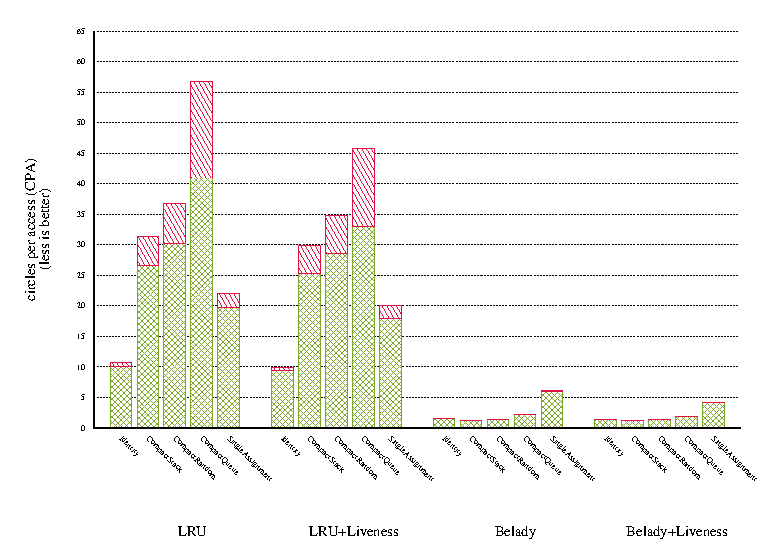
\includegraphics[width=\textwidth]{figs/plots/perf-misses-450-soplex.eps}
    \subcaption{Cache misses and cache hits}
  \end{subfigure}%
  \begin{subfigure}[b]{0.5\textwidth}%
    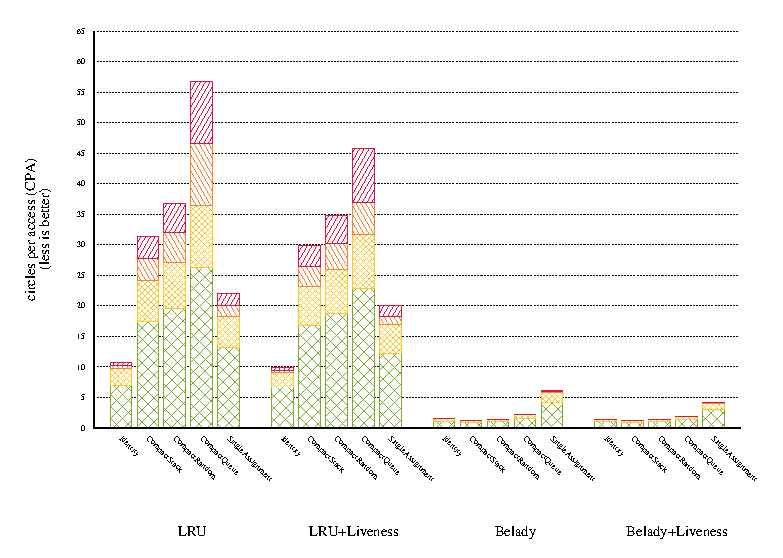
\includegraphics[width=\textwidth]{figs/plots/perf-450-soplex.eps}
    \subcaption{Types of memory operations}
  \end{subfigure}%
  \caption{Performance: 450.soplex}
  \label{fig:performance-450-soplex}
\end{figure}

\begin{figure}[!ht]
    \begin{subfigure}[b]{0.5\textwidth}%
    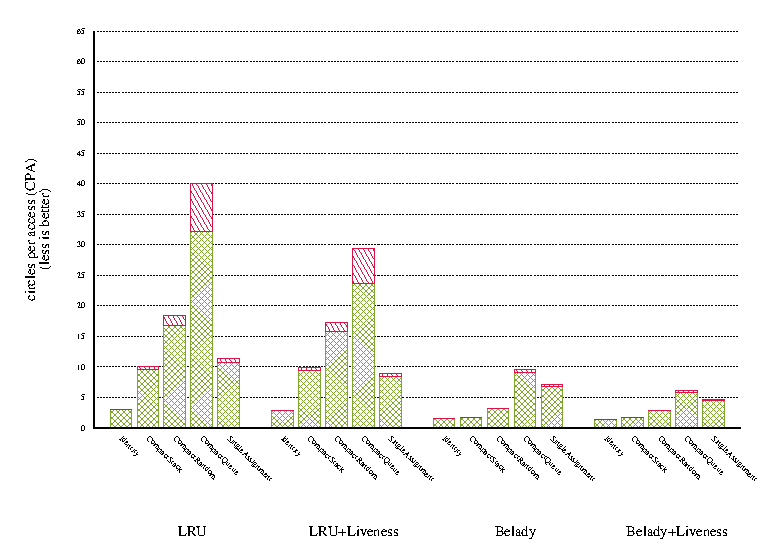
\includegraphics[width=\textwidth]{figs/plots/perf-misses-454-calculix.eps}
    \subcaption{Cache misses and cache hits}
  \end{subfigure}%
  \begin{subfigure}[b]{0.5\textwidth}%
    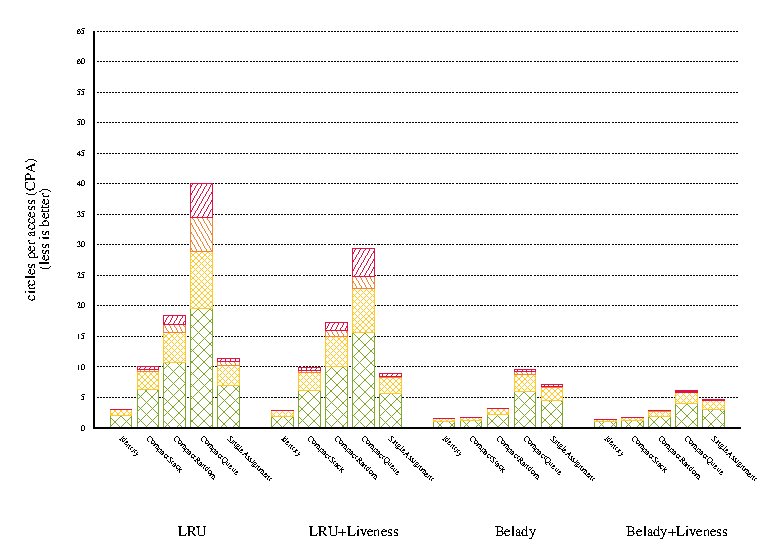
\includegraphics[width=\textwidth]{figs/plots/perf-454-calculix.eps}
    \subcaption{Types of memory operations}
  \end{subfigure}%
  \caption{Performance: 454.calculix}
  \label{fig:performance-454-calculix}
\end{figure}

\begin{figure}[!ht]
  \begin{subfigure}[b]{0.5\textwidth}%
    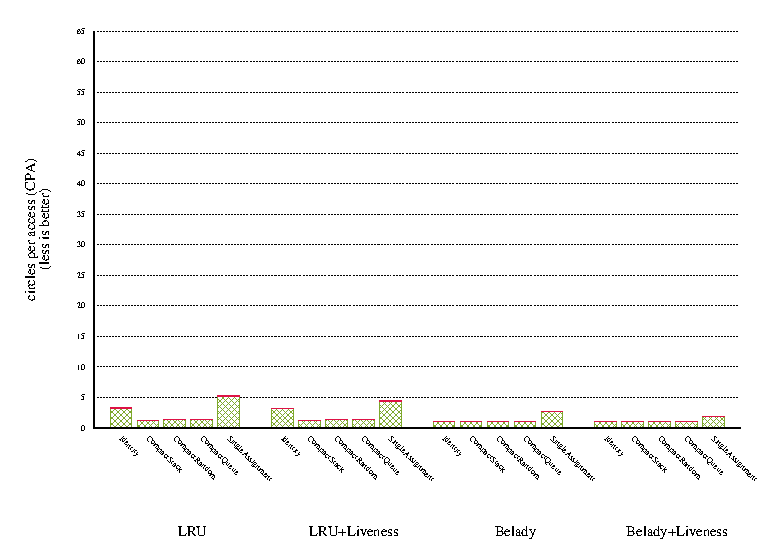
\includegraphics[width=\textwidth]{figs/plots/perf-misses-462-libquantum.eps}
    \subcaption{Cache misses and cache hits}
  \end{subfigure}%
  \begin{subfigure}[b]{0.5\textwidth}%
    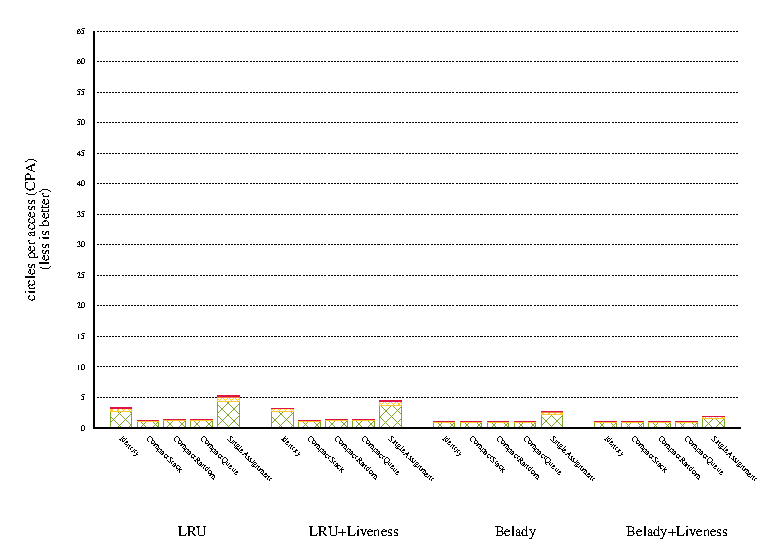
\includegraphics[width=\textwidth]{figs/plots/perf-462-libquantum.eps}
    \subcaption{Types of memory operations}
  \end{subfigure}%
  \caption{Performance: 462.libquantum}
  \label{fig:performance-462-libquantum}
\end{figure}

\begin{figure}[!ht]
  \begin{subfigure}[b]{0.5\textwidth}%
    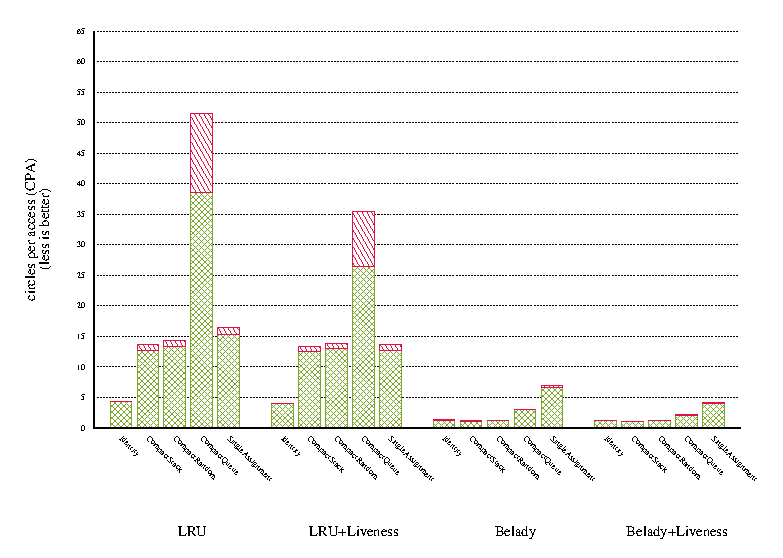
\includegraphics[width=\textwidth]{figs/plots/perf-misses-deltablue.eps}
    \subcaption{Cache misses and cache hits}
  \end{subfigure}%
  \begin{subfigure}[b]{0.5\textwidth}%
    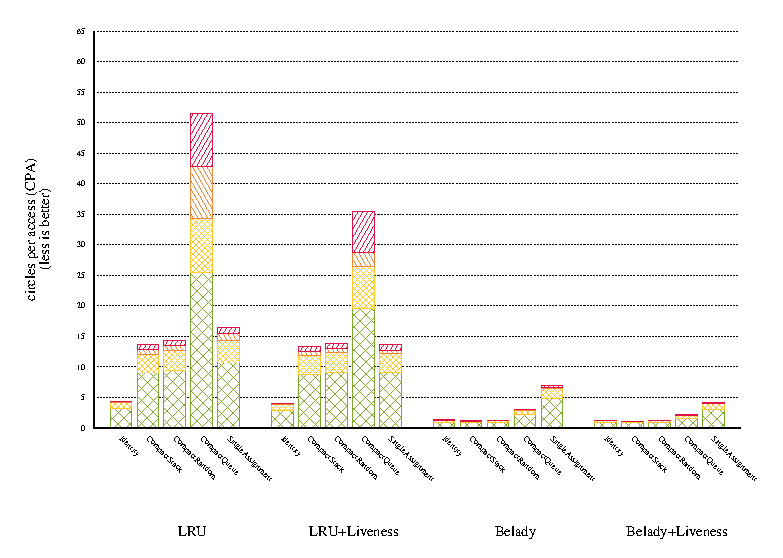
\includegraphics[width=\textwidth]{figs/plots/perf-deltablue.eps}
    \subcaption{Types of memory operations}
  \end{subfigure}%
  \caption{Performance: deltablue}
  \label{fig:performance-deltablue}
\end{figure}

\begin{figure}[!ht]
  \begin{subfigure}[b]{0.5\textwidth}%
    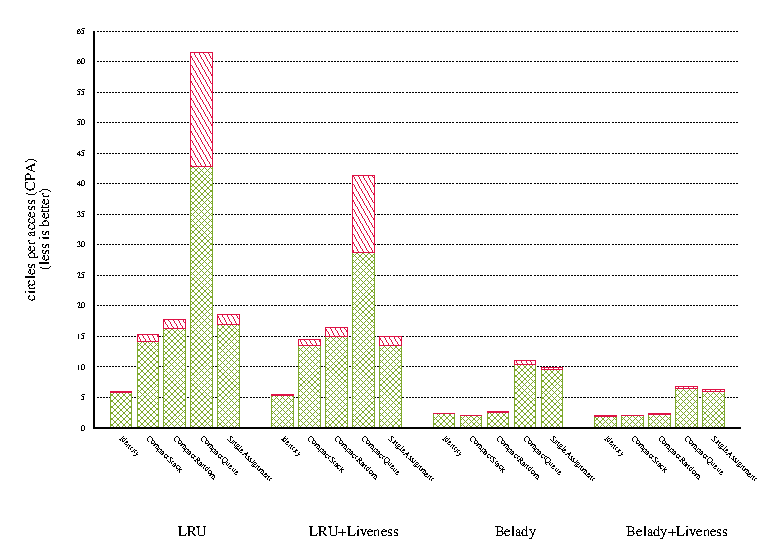
\includegraphics[width=\textwidth]{figs/plots/perf-misses-raytrace.eps}
    \subcaption{Cache misses and cache hits}
  \end{subfigure}%
  \begin{subfigure}[b]{0.5\textwidth}%
    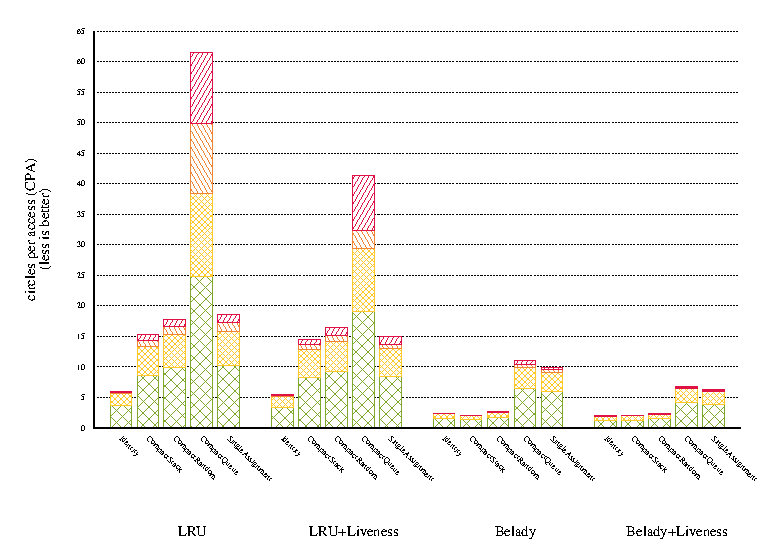
\includegraphics[width=\textwidth]{figs/plots/perf-raytrace.eps}
    \subcaption{Types of memory operations}
  \end{subfigure}%
  \caption{Performance: raytrace}
  \label{fig:performance-raytrace}
\end{figure}

\begin{figure}[!ht]
  \begin{subfigure}[b]{0.5\textwidth}%
    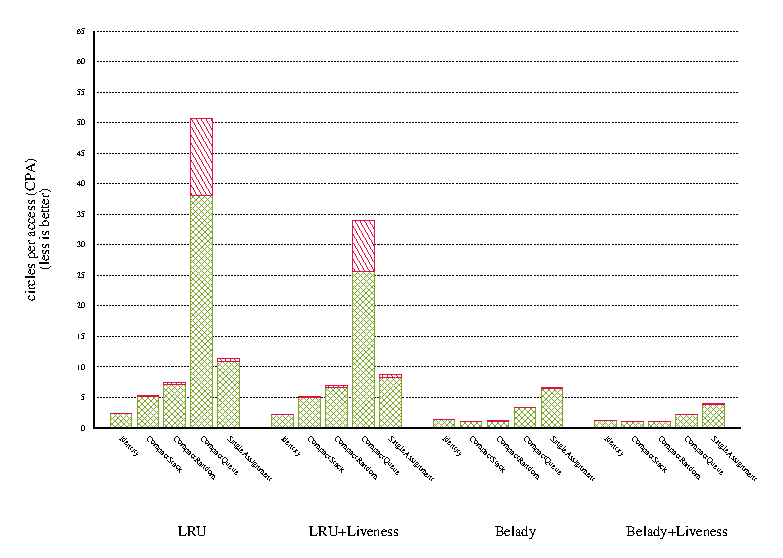
\includegraphics[width=\textwidth]{figs/plots/perf-misses-richards.eps}
    \subcaption{Cache misses and cache hits}
  \end{subfigure}%
  \begin{subfigure}[b]{0.5\textwidth}%
    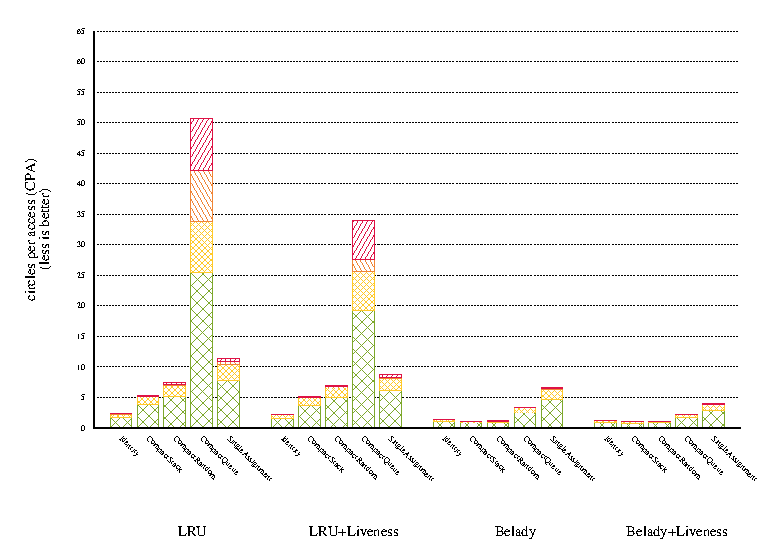
\includegraphics[width=\textwidth]{figs/plots/perf-richards.eps}
    \subcaption{Types of memory operations}
  \end{subfigure}%
  \caption{Performance: richards}
  \label{fig:performance-richards}
\end{figure}

\subsection{Speedup \& Compaction}\label{app:experiment-speedup-compaction}

\begin{figure}[!ht]
  \begin{subfigure}[b]{0.5\textwidth}%
    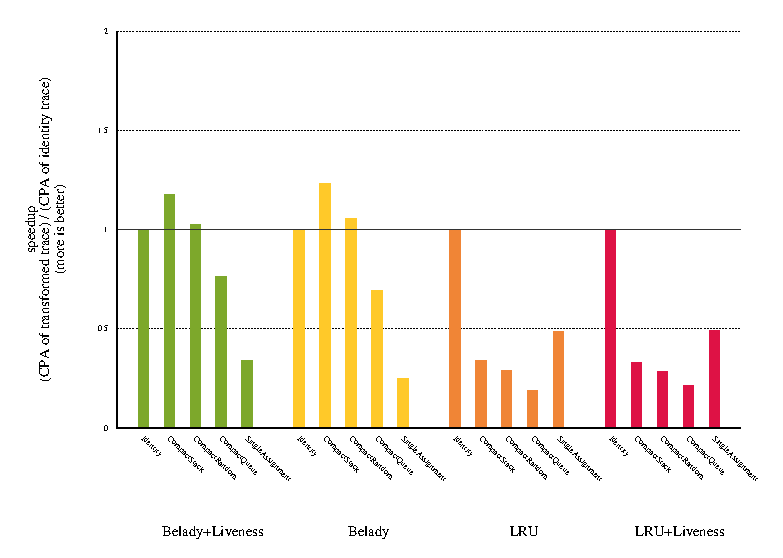
\includegraphics[width=\textwidth]{figs/plots/speedup-450-soplex.eps}
    \subcaption{Speedup}
  \end{subfigure}%
  \begin{subfigure}[b]{0.5\textwidth}%
    \includegraphics[width=\textwidth]{figs/plots/compaction-450-soplex.eps}
    \subcaption{Compaction}
  \end{subfigure}%
    \caption{Speedup \& Compaction: 450.soplex}
  \label{fig:speedup-compaction-450-soplex}
\end{figure}

\begin{figure}[!ht]
  \begin{subfigure}[b]{0.5\textwidth}%
    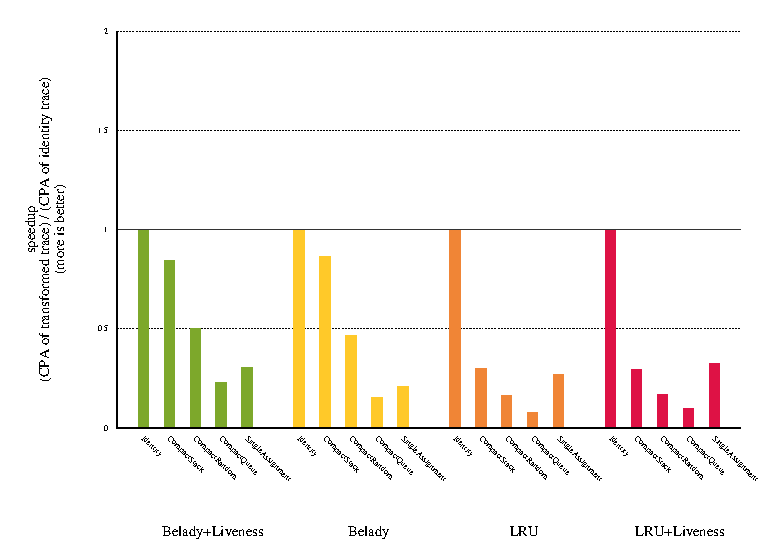
\includegraphics[width=\textwidth]{figs/plots/speedup-454-calculix.eps}
    \subcaption{Speedup}
  \end{subfigure}%
  \begin{subfigure}[b]{0.5\textwidth}%
    \includegraphics[width=\textwidth]{figs/plots/compaction-454-calculix.eps}
    \subcaption{Compaction}
  \end{subfigure}%
    \caption{Speedup \& Compaction: 454.calculix}
  \label{fig:speedup-compaction-454-calculix}
\end{figure}

\begin{figure}[!ht]
  \begin{subfigure}[b]{0.5\textwidth}%
    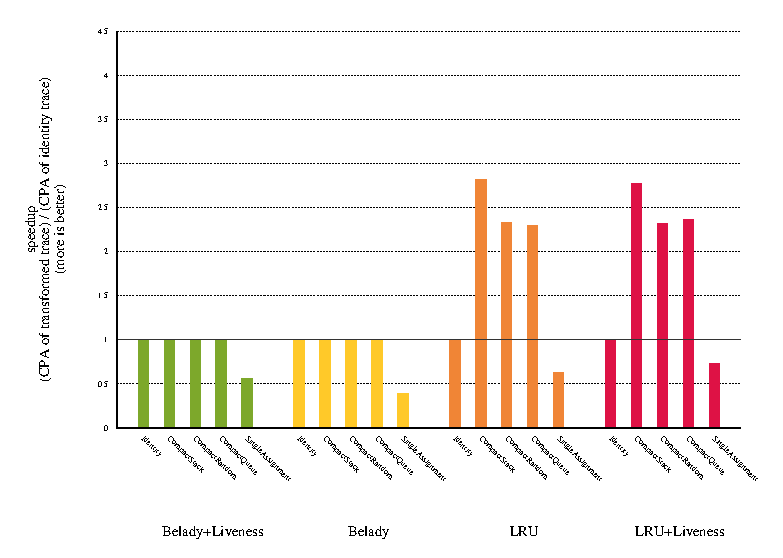
\includegraphics[width=\textwidth]{figs/plots/speedup-462-libquantum.eps}
    \subcaption{Speedup}
  \end{subfigure}%
  \begin{subfigure}[b]{0.5\textwidth}%
    \includegraphics[width=\textwidth]{figs/plots/compaction-462-libquantum.eps}
    \subcaption{Compaction}
  \end{subfigure}%
    \caption{Speedup \& Compaction: 462.libquantum}
  \label{fig:speedup-compaction-462-libquantum}
\end{figure}

\begin{figure}[!ht]
  \begin{subfigure}[b]{0.5\textwidth}%
    \includegraphics[width=\textwidth]{figs/plots/speedup-deltablue.eps}
    \subcaption{Speedup}
  \end{subfigure}%
  \begin{subfigure}[b]{0.5\textwidth}%
    \includegraphics[width=\textwidth]{figs/plots/compaction-deltablue.eps}
    \subcaption{Compaction}
  \end{subfigure}%
    \caption{Speedup \& Compaction: deltablue}
  \label{fig:speedup-compaction-deltablue}
\end{figure}

\begin{figure}[!ht]
  \begin{subfigure}[b]{0.5\textwidth}%
    \includegraphics[width=\textwidth]{figs/plots/speedup-raytrace.eps}
    \subcaption{Speedup}
  \end{subfigure}%
  \begin{subfigure}[b]{0.5\textwidth}%
    \includegraphics[width=\textwidth]{figs/plots/compaction-raytrace.eps}
    \subcaption{Compaction}
  \end{subfigure}%
    \caption{Speedup \& Compaction: raytrace}
  \label{fig:speedup-compaction-raytrace}
\end{figure}

\begin{figure}[!ht]
  \begin{subfigure}[b]{0.5\textwidth}%
    \includegraphics[width=\textwidth]{figs/plots/speedup-richards.eps}
    \subcaption{Speedup}
  \end{subfigure}%
  \begin{subfigure}[b]{0.5\textwidth}%
    \includegraphics[width=\textwidth]{figs/plots/compaction-richards.eps}
    \subcaption{Compaction}
  \end{subfigure}%
  \caption{Speedup \& Compaction: richards}
  \label{fig:speedup-compaction-richards}
\end{figure}

% \clearpage
\section{Digression on Caches}

This experimental section is distinguished into 2 parts. First we show a
few different opportunities to access a linked list, and an array,
respectively. Allows keeping our purpose in mind, we want to illustrate
the cache hierarchy. Secondly, we go into details and clarify a raising
question. Which finally leads to the answer we are looking for.

All experiments were executed on a MacBook Pro with a Intel(R) Core(TM)
i5-3230M CPU @ 2.60GHz and 3 cache levels (L1d=32KB, L1i=32KB, L2=256KB,
and L3=3MB). During the experiments there were other processes running
on the MacBook, this is why these results should be seen as proof of
concept.

\subsection{Configuration}\label{configuration-3}

The configuration is for all experiments identical.

\begin{longtable}[c]{@{}cccc@{}}
\toprule
Reps & Operations & Working Set Sizes & Addresses\tabularnewline
\midrule
\endhead
3 & 234 & 210 - 228 & 228\tabularnewline
\bottomrule
\end{longtable}

We are aware that the number of repetitions is very small, but we
consider these experiments as a \emph{proof of concept}. So 3
repetitions should be good enough.

There are parameters listed within the configuration files which are
\textbf{not} used for this experiments! These are only listed to keep
the experimental framework working.

\begin{itemize}
\tightlist
\item
  Fragmentation factor
\item
  Store ratio
\end{itemize}

As explained above we generate for each working set size a standalone
\texttt{C} file. which is complied with \texttt{gcc} in version 4.8.5
with following compiler flags \texttt{-std=c99} and \texttt{-O0}.

\hypertarget{access-opportunities}{\subsection{Access
opportunities}\label{access-opportunities}}

\hypertarget{linked-list}{\paragraph{Linked List}\label{linked-list}}

This section presents code snippets and performance results of accessing
a linked list to illustrate the cache hierarchy.

\hypertarget{sequential-access-with-2-loops}{\subparagraph{Sequential
access with 2 loops}\label{sequential-access-with-2-loops}}

The code snippet below shows how to access the linked list in a
sequential manner. All list elements are sequentially linked
corresponding to there position in (contiguous) memory. This approach
uses two nested loops.

\begin{Shaded}
\begin{Highlighting}[]
\DataTypeTok{static} \DataTypeTok{uint64_t} \NormalTok{access_read() \{}
  \KeywordTok{struct} \NormalTok{l * cur = &list[}\DecValTok{0}\NormalTok{];}
  \DataTypeTok{uint64_t} \NormalTok{start = getTimeMicrosecs();}
  \KeywordTok{for}\NormalTok{(}\DataTypeTok{int} \NormalTok{i = }\DecValTok{0}\NormalTok{; i < ITERS; i++)}
  \NormalTok{\{}
    \KeywordTok{for}\NormalTok{(}\DataTypeTok{int} \NormalTok{e = }\DecValTok{0}\NormalTok{; e < ELEMS; e++)}
    \NormalTok{\{}
      \NormalTok{cur = cur->n;}
      \NormalTok{(}\DataTypeTok{void}\NormalTok{)cur->pad[}\DecValTok{0}\NormalTok{];}
    \NormalTok{\}}
  \NormalTok{\}}
  \KeywordTok{return} \NormalTok{getTimeMicrosecs() - start;}
\NormalTok{\}}
\end{Highlighting}
\end{Shaded}

\Cref{ll-seqread-nl} presents the performance of the code above. As expected
the cache hierarchy is observable. However, performance is not that
good. How poor it really is illustrates the next experiment.

\begin{figure}[htbp]
\centering
\includegraphics{appendix/plots-cache-measurements/plot-linked-list-2-loops}
\caption{Linked List, Sequential Read, and Nested Loop}
\label{ll-seqread-nl}
\end{figure}

\hypertarget{sequential-access-with-single-loop}{\subparagraph{Sequential
access with single loop}\label{sequential-access-with-single-loop}}

This approach is similar to the one above, but instead of two nested
loops a single loop is used. All list elements are sequentially linked
corresponding to there position in (contiguous) memory.

\begin{Shaded}
\begin{Highlighting}[]
\DataTypeTok{static} \DataTypeTok{uint64_t} \NormalTok{access_read() \{}
  \KeywordTok{struct} \NormalTok{l * cur = &list[}\DecValTok{0}\NormalTok{];}
  \DataTypeTok{uint64_t} \NormalTok{start = getTimeMicrosecs();}
  \KeywordTok{for}\NormalTok{(}\DataTypeTok{int} \NormalTok{i = }\DecValTok{0}\NormalTok{; i < ITERS * ELEMS; i++)}
  \NormalTok{\{}
    \NormalTok{cur = cur->n;}
    \NormalTok{(}\DataTypeTok{void}\NormalTok{)cur->pad[}\DecValTok{0}\NormalTok{];}
  \NormalTok{\}}
  \KeywordTok{return} \NormalTok{getTimeMicrosecs() - start;}
\NormalTok{\}}
\end{Highlighting}
\end{Shaded}

\Cref{app:ll-seqread-sl} illustrates the performance of the code from above. As
expected the results shows the typical shape. Remember the experiment
was not the only job running, this is why the shape not totally sharp.
This figure is used as baseline for the following experiments.

\begin{figure}[htbp]
\centering
\includegraphics{appendix/plots-cache-measurements/plot-linked-list}
\caption{Linked List, Sequential Read, and Single Loop}
\label{app:ll-seqread-sl}
\end{figure}

\hypertarget{array}{\paragraph{Array}\label{array}}

This section presents different ways to compute the index of the array.
The aim is illustrate the influence of computing the index of the
current element on the actual measurements.

\hypertarget{sequential-access-with-2-loops-1}{\subparagraph{Sequential
access with 2 loops}\label{sequential-access-with-2-loops-1}}

The code snippet below shows how the array is accessed. This approach
uses to nested loop. The outer-one determines the number accesses on a
single element with the array. The inner-one ensures that keep walking
through the array.

\begin{Shaded}
\begin{Highlighting}[]
\DataTypeTok{static} \DataTypeTok{uint64_t} \NormalTok{access_read() \{}
  \DataTypeTok{uint64_t} \NormalTok{start = getTimeMicrosecs();}
  \KeywordTok{for}\NormalTok{(}\DataTypeTok{int} \NormalTok{i = }\DecValTok{0}\NormalTok{; i < ITERS; i++)}
    \KeywordTok{for}\NormalTok{(}\DataTypeTok{int} \NormalTok{j = }\DecValTok{0}\NormalTok{; j < ELEMS; j++)}
      \NormalTok{(}\DataTypeTok{void}\NormalTok{)list[j].pad[}\DecValTok{0}\NormalTok{];}
  \KeywordTok{return} \NormalTok{getTimeMicrosecs() - start;}
\NormalTok{\}}
\end{Highlighting}
\end{Shaded}

\Cref{app:arr-seqread-nl} presents the performance of the code above. Obviously
the cache hierarchy is not observable. Instead the performance seams to
be independent of the working set size. We continue with a few more
experiments on array before taking a closer look at this effect.

\begin{figure}[htbp]
\centering
\includegraphics{appendix/plots-cache-measurements/plot-array-2-loops}
\caption{Array, Sequential Read, and Nested Loop}
\label{app:arr-seqread-nl}
\end{figure}

\hypertarget{sequential-access-with-single-loop-and-modulo}{\subparagraph{Sequential
access with single loop and
modulo}\label{sequential-access-with-single-loop-and-modulo}}

The code snippet below illustrates an approach which uses only one loop.
This requires a modulo operation to ensure to stay within the array
bounds.

\begin{Shaded}
\begin{Highlighting}[]
\DataTypeTok{static} \DataTypeTok{uint64_t} \NormalTok{access_read() \{}
  \DataTypeTok{uint64_t} \NormalTok{start = getTimeMicrosecs();}
  \KeywordTok{for}\NormalTok{(}\DataTypeTok{int} \NormalTok{i = }\DecValTok{0}\NormalTok{; i < ITERS * ELEMS; i++)}
    \NormalTok{(}\DataTypeTok{void}\NormalTok{)list[i%ELEMS].pad[}\DecValTok{0}\NormalTok{];}
  \KeywordTok{return} \NormalTok{getTimeMicrosecs() - start;}
\NormalTok{\}}
\end{Highlighting}
\end{Shaded}

\Cref{app:arr-seqread-sl} shows the performance of the code above. Again the
performance seams to be independent of the working set size. However,
there is a significant performance improvement compared to the approach
with two loops.

\begin{figure}[htbp]
\centering
\includegraphics{appendix/plots-cache-measurements/plot-array-modulo-seq}
\caption{Array, Sequential Read, and Single Loop}
\label{app:arr-seqread-sl}
\end{figure}

\hypertarget{sequential-access-with-single-loop-and-modulo-linked-list-style}{\subparagraph{Sequential
access with single loop and modulo (linked list
style)}\label{sequential-access-with-single-loop-and-modulo-linked-list-style}}

The code snipped below presents an approach which used only one loop,
which requires a modulo operation to care about the array bounds.
Further, the coding style is like used a linked lists. There is an
additional variable \texttt{cur} which holds the address of the element
to access. The reason for this experiment that all experiments with
arrays so far do not show the cache hierarchy. To become as comparable
as possible we use this linked list like syntax.

\begin{Shaded}
\begin{Highlighting}[]
\DataTypeTok{static} \DataTypeTok{uint64_t} \NormalTok{access_read() \{}
  \KeywordTok{struct} \NormalTok{l * cur = &list[}\DecValTok{0}\NormalTok{];}
  \DataTypeTok{uint64_t} \NormalTok{start = getTimeMicrosecs();}
  \KeywordTok{for}\NormalTok{(}\DataTypeTok{int} \NormalTok{i = }\DecValTok{0}\NormalTok{; i < ITERS * ELEMS; i++)\{}
    \NormalTok{cur = &list[i%ELEMS];}
    \NormalTok{(}\DataTypeTok{void}\NormalTok{)cur->pad[}\DecValTok{0}\NormalTok{];}
  \NormalTok{\}}
  \KeywordTok{return} \NormalTok{getTimeMicrosecs() - start;}
\NormalTok{\}}
\end{Highlighting}
\end{Shaded}

\Cref{app:array-seqread-sl} below shows the performance of the code above. Again the
performance seams to be independent of the working set size. However,
the performance is slightly worse than the performance of the previous
experiment. The explanation is as simple as: It is requires to store the
address within \texttt{cur}, the approach from above computes address
and stores it in a register.

\begin{figure}[htbp]
\centering
\includegraphics{appendix/plots-cache-measurements/plot-array-modulo-seq-2}
\caption{Array, Sequential Read, and Single Loop}
\label{app:array-seqread-sl}
\end{figure}

\hypertarget{sequential-access-with-single-loop-and-modulo-read-whole-payload}{\subparagraph{Sequential
access with single loop and modulo (read whole
payload)}\label{sequential-access-with-single-loop-and-modulo-read-whole-payload}}

The code snippet below presents an approach similar to those from above
with one difference: The whole payload is read (instead of simply
reading on element).

\begin{Shaded}
\begin{Highlighting}[]
\DataTypeTok{static} \DataTypeTok{uint64_t} \NormalTok{access_read() \{}
  \KeywordTok{struct} \NormalTok{l * cur = &list[}\DecValTok{0}\NormalTok{];}
  \DataTypeTok{uint64_t} \NormalTok{start = getTimeMicrosecs();}
  \KeywordTok{for}\NormalTok{(}\DataTypeTok{int} \NormalTok{i = }\DecValTok{0}\NormalTok{; i < ITERS * ELEMS; i++)\{}
    \NormalTok{cur = &list[i%ELEMS];}
    \KeywordTok{for}\NormalTok{(}\DataTypeTok{int} \NormalTok{j = }\DecValTok{0}\NormalTok{; j < NPAD; j++)}
      \NormalTok{(}\DataTypeTok{void}\NormalTok{)cur->pad[j];}
  \NormalTok{\}}
  \KeywordTok{return} \NormalTok{getTimeMicrosecs() - start;}
\NormalTok{\}}
\end{Highlighting}
\end{Shaded}

\Cref{app:array-seqreadall-sl} shows the result of the code from above. It was
expected to see the cache hierarchy, because we read the whole array
which is definitely larger than the cache. Nevertheless, the result is
the same as for the other array experiments. The only difference is the
worse performance yield by the additional loop.

\begin{figure}[htbp]
\centering
\includegraphics{appendix/plots-cache-measurements/plot-array-modulo-seq-read-all}
\caption{Array, Sequential Read All, and Single Loop}
\label{app:array-seqreadall-sl}
\end{figure}

\hypertarget{random-access-with-single-loop-and-modulo}{\subparagraph{Random
access with single loop and
modulo}\label{random-access-with-single-loop-and-modulo}}

The code snippet below presents an approach similar to those from above
with one difference: Now the array elements are access in a random
order. \texttt{mapper} contains a randomly chosen permutation of all
array indexes.

\begin{Shaded}
\begin{Highlighting}[]
\DataTypeTok{static} \DataTypeTok{uint64_t} \NormalTok{access_read() \{}
  \KeywordTok{struct} \NormalTok{l * cur = &list[}\DecValTok{0}\NormalTok{];}
  \DataTypeTok{uint64_t} \NormalTok{start = getTimeMicrosecs();}
  \KeywordTok{for}\NormalTok{(}\DataTypeTok{int} \NormalTok{i = }\DecValTok{0}\NormalTok{; i < ITERS * ELEMS; i++)\{}
    \NormalTok{cur = &list[mapper[i%ELEMS]];}
    \NormalTok{(}\DataTypeTok{void}\NormalTok{)cur->pad[}\DecValTok{0}\NormalTok{];}
  \NormalTok{\}}
  \KeywordTok{return} \NormalTok{getTimeMicrosecs() - start;}
\NormalTok{\}}
\end{Highlighting}
\end{Shaded}

The performance result is shown in \Cref{app:arr-randread-sl}. The random access order is chosen
to get rid of pre-fetching which could probably influence the execution
time. But even with random access on the array we cannot observer the
cache hierarchy. It is comparable to \emph{sequential access with single
loop and modulo (linked list style)}.

\begin{figure}[htbp]
\centering
\includegraphics{appendix/plots-cache-measurements/plot-array-modulo-rand}
\caption{Array, Random Read, and Single Loop}
\label{app:arr-randread-sl}
\end{figure}

\hypertarget{summary-1}{\paragraph{Summary}\label{summary-1}}

We presented experiments on accessing two different data structures,
linked lists, and arrays, respectively. For linked lists we showed that
there is a huge performance difference in using nested loops or just a
single loop. This fact is not super surprising, but nevertheless
important to keep in mind. Also for arrays is shown that 2 nested loops
perform do not perform well. Further, we tried to measure the cache
hierarchy using just an array. Without success. Instead our experiments
show the performance differences of the different ways to access an
array. The following section will go into details why performance seams
to be independent of the working set size.

\hypertarget{the-problem}{\subsection{The problem}\label{the-problem}}

\hypertarget{definition}{\subsection{Definition}\label{definition}}

The performance curve of all experiments with array only is close to a
horizontal line, and this is unexpected behavior. It seams to be
independent of the working set size. The expected behavior would be
similar to the linked list experiments, which illustrate the cache
hierarchy.

\subsection{Analysis}\label{analysis-1}

In this section we investigate the unexpected behavior of our array
experiments from above. These experiments present constant performance
independent of the working set size.

\hypertarget{assembly-code-analysis}{\paragraph{Assembly code
analysis}\label{assembly-code-analysis}}

To simplify as much as possible we inspect only 2 code snippets from
above: - Linked list with single loop and - Array with single loop in
linked list style.

These two are the most similar one so optimal for comparison. We
disassembled the executables complied on the MacBook mentioned above.
For disassembling we are using an on-line disassembler:
\url{https://onlinedisassembler.com}.

\textbf{Linked list: C code}

\begin{Shaded}
\begin{Highlighting}[]
\DataTypeTok{static} \DataTypeTok{uint64_t} \NormalTok{access_read() \{}
  \KeywordTok{struct} \NormalTok{l * cur = &list[}\DecValTok{0}\NormalTok{];}
  \DataTypeTok{uint64_t} \NormalTok{start = getTimeMicrosecs();}
  \KeywordTok{for}\NormalTok{(}\DataTypeTok{int} \NormalTok{i = }\DecValTok{0}\NormalTok{; i < ITERS * ELEMS; i++)\{}
    \NormalTok{cur = cur->n;}
    \NormalTok{(}\DataTypeTok{void}\NormalTok{)cur->pad[}\DecValTok{0}\NormalTok{];}
  \NormalTok{\}}
  \KeywordTok{return} \NormalTok{getTimeMicrosecs() - start;}
\NormalTok{\}}
\end{Highlighting}
\end{Shaded}

\textbf{Linked list: Assembly}

\begin{verbatim}
100000ec0 <_access_read>:
100000ec0 55                     push   %rbp
100000ec1 4889e5                 mov    %rsp,         %rbp
100000ec4 4883ec20               sub    $0x20,        %rsp
100000ec8 488d0551010000         lea    0x151(%rip),  %rax # 0x100001020<_list>
100000ecf 488945f8               mov    %rax,         -0x8(%rbp)
100000ed3 e858000000             callq  0x100000f30   <_getTimeMicrosecs>
100000ed8 488945f0               mov    %rax,         -0x10(%rbp)
100000edc c745ec00000000         movl   $0x0,         -0x14(%rbp)
100000ee3 48b80000000004000000   movabs $0x400000000, %rax
100000eed 48634dec               movslq -0x14(%rbp),  %rcx
100000ef1 4839c1                 cmp    %rax,         %rcx
100000ef4 0f8319000000           jae    0x100000f13
100000efa 488b45f8               mov    -0x8(%rbp),   %rax
100000efe 488b00                 mov    (%rax),       %rax
100000f01 488945f8               mov    %rax,         -0x8(%rbp)
100000f05 8b45ec                 mov    -0x14(%rbp),  %eax
100000f08 83c001                 add    $0x1,         %eax
100000f0b 8945ec                 mov    %eax,         -0x14(%rbp)
100000f0e e9d0ffffff             jmpq   0x100000ee3
100000f13 e818000000             callq  0x100000f30   <_getTimeMicrosecs>
100000f18 482b45f0               sub    -0x10(%rbp),  %rax
100000f1c 4883c420               add    $0x20,        %rsp
100000f20 5d                     pop    %rbp
100000f21 c3                     retq   
\end{verbatim}

\textbf{Array: C code}

\begin{Shaded}
\begin{Highlighting}[]
\NormalTok{...}
\DataTypeTok{static} \DataTypeTok{uint64_t} \NormalTok{access_read() \{}
  \KeywordTok{struct} \NormalTok{l * cur = &list[}\DecValTok{0}\NormalTok{];}
  \DataTypeTok{uint64_t} \NormalTok{start = getTimeMicrosecs();}
  \KeywordTok{for}\NormalTok{(}\DataTypeTok{int} \NormalTok{i = }\DecValTok{0}\NormalTok{; i < ITERS * ELEMS; i++)\{}
    \NormalTok{cur = &list[i%ELEMS];}
    \NormalTok{(}\DataTypeTok{void}\NormalTok{)cur->pad[}\DecValTok{0}\NormalTok{];}
  \NormalTok{\}}
  \KeywordTok{return} \NormalTok{getTimeMicrosecs() - start;}
\NormalTok{\}}
\end{Highlighting}
\end{Shaded}

\textbf{Array: Assembly}

\begin{verbatim}
100000eb0 <_access_read>:
100000eb0 55                     push   %rbp
100000eb1 4889e5                 mov    %rsp,         %rbp
100000eb4 4883ec20               sub    $0x20,        %rsp
100000eb8 488d0561010000         lea    0x161(%rip),  %rax # 0x100001020<_list>
100000ebf 488945f8               mov    %rax,         -0x8(%rbp)
100000ec3 e868000000             callq  0x100000f30   <_getTimeMicrosecs>
100000ec8 488945f0               mov    %rax,         -0x10(%rbp)
100000ecc c745ec00000000         movl   $0x0,         -0x14(%rbp)
100000ed3 48b80000000004000000   movabs $0x400000000, %rax
100000edd 48634dec               movslq -0x14(%rbp),  %rcx
100000ee1 4839c1                 cmp    %rax,         %rcx
100000ee4 0f8328000000           jae    0x100000f12
100000eea 488d052f010000         lea    0x12f(%rip),  %rax # 0x100001020<_list>
100000ef1 48634dec               movslq -0x14(%rbp),  %rcx
100000ef5 4883e10f               and    $0xf,         %rcx
100000ef9 48c1e106               shl    $0x6,         %rcx
100000efd 4801c8                 add    %rcx,         %rax
100000f00 488945f8               mov    %rax,         -0x8(%rbp)
100000f04 8b45ec                 mov    -0x14(%rbp),  %eax
100000f07 83c001                 add    $0x1,         %eax
100000f0a 8945ec                 mov    %eax,         -0x14(%rbp)
100000f0d e9c1ffffff             jmpq   0x100000ed3
100000f12 e819000000             callq  0x100000f30   <_getTimeMicrosecs>
100000f17 482b45f0               sub    -0x10(%rbp),  %rax
100000f1b 4883c420               add    $0x20,        %rsp
100000f1f 5d                     pop    %rbp
100000f20 c3                     retq   
\end{verbatim}

Now we remove everything this two code snippets have in common and is
not required for our analysis. What remains should help us to understand
the difference between array and linked list. Hopefully it offers some
answers about the performance differences.

Obviously, there are only a few lines which distinguishes the code
snippets. We take only a look at the code within the loop.

The code for the linked list is quite strait. First the address of
\texttt{cur} is loaded into \texttt{rax}. Next the address of \texttt{n}
is computed. Since \texttt{n} is the first element within the
\texttt{struct} this is identical with the address of \texttt{cur}.
Finally, the address stored in \texttt{n} is moved/assigned to
\texttt{cur} itself. For reading the first element of the payload there
is no command.

The code for the array consists of a few more lines. The most important
command is the \texttt{lea} command. \texttt{lea} is a special command
available on Intel x86 architectures. This is a so called \textbf{load
effective address} instruction, designed specially of arrays. It
performs a calculation of the effective operand address, but instead of
acting on that memory location, it loads the address that would have
been accessed into a register. This and the fact that there is no
assembly instruction generated for
\texttt{(void)\ cur-\textgreater{}pad{[}0{]}} are the reasons why the
performance of arrays seams to be independent of working set size. There
is no actual memory access, the way we want it. The following
instructions do the modulo computation and finally assign the computed
address to \texttt{cur} again.

\begin{verbatim}
# linked list
<_access_read>:
loop:     ...
          jae    end_loop
          mov    -0x8(%rbp),   %rax       # load address of cur
          mov    (%rax),       %rax       # compute address of n
          mov    %rax,         -0x8(%rbp) # assignment: cur = cur->n
                                          # (void) cur->pad[0]
          ...                             # increment loop counter
          jmpq   loop
end_loop: ...

# array
<_access_read>:
loop:     ...
          jae    end_loop
          lea    0x12f(%rip),  %rax       # load list address
          movslq -0x14(%rbp),  %rcx       # load max. loop counter
          and    $0xf,         %rcx       # compute: i%ELEMS
          shl    $0x6,         %rcx       # compute: i%ELEMS
          add    %rcx,         %rax       # compute address of list element
          mov    %rax,         -0x8(%rbp) # assignment: cur = &list[i%ELEMS]
                                          # (void) cur->pad[0]
          ...                             # increment loop counter
          jmpq   loop
end_loop: ...
\end{verbatim}

\textbf{Explanations:} - Source:
\href{https://en.wikipedia.org/wiki/X86_instruction_listings}{Wikipedia}
- Variables + \texttt{-0x8(\%rbp)}: current element
(\texttt{struct\ l\ *cur}) + \texttt{-0x14(\%rbp)}: loop counter
(\texttt{int\ i}) + \texttt{0x12f(\%rip)}: the list of structs
(\texttt{struct\ list{[}ELEMS{]}}) + \texttt{\$0xf}: number of elements
(\texttt{ELEMS} = 16) + \texttt{\$0x6}: decimal number \texttt{6} -
Registers + \texttt{rax}, \texttt{rbx}, \texttt{rcx}: 64-bit register +
\texttt{rbp}: 64-bit register, holds method local variables +
\texttt{rip}: 64-bit instruction pointer register. only in the 64-bit
mode it is possible to reference data relative to the instruction
pointer, less copying of data is required. - Commands +
\texttt{movslq\ S,\ R}: Move sign-extended double word + \texttt{shl}:
Shift left + \texttt{lea}: ``Some instruction set architectures, such as
Intel x86 {[}\ldots{}{]}, have a \textbf{Load effective address}
instruction.{[}\ldots{}{]} This performs a calculation of the effective
operand address, but instead of acting on that memory location, it loads
the address that would have been accessed into a register.
{[}\ldots{}{]}'' \emph{Source:
\href{https://en.wikipedia.org/wiki/Addressing_mode\#Useful_side_effect}{Wikipedia}}

\hypertarget{further-investigations}{\paragraph{Further
investigations}\label{further-investigations}}

One issue which is identified above is that probably there are no
Assembly commands generated for the \texttt{C} code line
\texttt{(void)\ cur-\textgreater{}pad{[}0{]};}. This is not only an
issue of our array experiments. Also for the linked list experiments
these Assembly commands are missing. For simplicity reason the following
investigations are based on the linked list code. Since there are less
Assembly commands generated in total.

\hypertarget{without-accessing-pad}{\subparagraph{\texorpdfstring{Without
accessing
\texttt{pad}}{Without accessing pad}}\label{without-accessing-pad}}

This first experiment is used to confirm or refute the hypotheses that
the compiler does not generate Assembly commands for the access of
\texttt{pad}. For this purpose we remove the line
\texttt{(void)\ cur-\textgreater{}pad{[}0{]};} for the \texttt{C} code
re-compile it and again inspect it with disassembler used before
(\url{https://onlinedisassembler.com}). Both code snippets are presented
below.

\begin{Shaded}
\begin{Highlighting}[]
\DataTypeTok{static} \DataTypeTok{uint64_t} \NormalTok{access_read() \{}
  \KeywordTok{struct} \NormalTok{l * cur = &list[}\DecValTok{0}\NormalTok{];}
  \DataTypeTok{uint64_t} \NormalTok{start = getTimeMicrosecs();}
  \KeywordTok{for}\NormalTok{(}\DataTypeTok{int} \NormalTok{i = }\DecValTok{0}\NormalTok{; i < ITERS * ELEMS; i++)\{}
    \NormalTok{cur = cur->n;}
  \NormalTok{\}}
  \KeywordTok{return} \NormalTok{getTimeMicrosecs() - start;}
\NormalTok{\}}
\end{Highlighting}
\end{Shaded}

\begin{verbatim}
<_access_read>:
loop:     ...
          jae end_loop
          mov -0x8(%rbp),     %rax        # load address of cur
          mov (%rax),         %rax        # compute address of n
          mov %rax,           -0x8(%rbp)  # assignment: cur = cur->n
          ...                             # increment loop counter
          jmpq loop
end_loop: ...
\end{verbatim}

(\href{https://github.com/cksystemsgroup/SemanticLocality/blob/localizer/experiments/localizer/__meeting_20161130/assembly_tests/exp_ll_remove_cmd.txt}{complete
assembly code})

Obviously, the disassembled code is identically with the code generated
with one line more. This is why the Assembly code from above confirms
our hypotheses: There is no code generated for the \texttt{C} code
\texttt{(void)\ cur-\textgreater{}pad{[}0{]};}. Next we want to know it
the cast is the reason or line itself.

\hypertarget{remove-cast}{\subparagraph{Remove cast}\label{remove-cast}}

To find out why the compiler ignores
\texttt{(void)\ cur-\textgreater{}pad{[}0{]};} we remove the cast. This
raises a compiler warning of an unused variable.

\begin{Shaded}
\begin{Highlighting}[]
\DataTypeTok{static} \DataTypeTok{uint64_t} \NormalTok{access_read() \{}
  \KeywordTok{struct} \NormalTok{l * cur = &list[}\DecValTok{0}\NormalTok{];}
  \DataTypeTok{uint64_t} \NormalTok{start = getTimeMicrosecs();}
  \KeywordTok{for}\NormalTok{(}\DataTypeTok{int} \NormalTok{i = }\DecValTok{0}\NormalTok{; i < ITERS * ELEMS; i++)\{}
    \NormalTok{cur = cur->n;}
    \NormalTok{cur->pad[}\DecValTok{0}\NormalTok{];}
  \NormalTok{\}}
  \KeywordTok{return} \NormalTok{getTimeMicrosecs() - start;}
\NormalTok{\}}
\end{Highlighting}
\end{Shaded}

\begin{verbatim}
<_access_read>:
loop:     ...
          jae    end_loop
          mov    -0x8(%rbp),  %rax        # load address of cur
          mov    (%rax),      %rax        # compute address of n
          mov    %rax,        -0x8(%rbp)  # assignment: cur = cur->n
          ...                             # increment loop counter
          jmpq   loop
end_loop: ...
\end{verbatim}

(\href{https://github.com/cksystemsgroup/SemanticLocality/blob/localizer/experiments/localizer/__meeting_20161130/assembly_tests/exp_ll_no_cast.txt}{complete
assembly code})

This experiment shows that the casting nothing changes. The only
recognizable effect is that the compiler does not throw the warning
about a unused variable. Next we want to force the compiler to generate
code.

\hypertarget{add-assignment}{\subparagraph{Add
assignment}\label{add-assignment}}

The previous two experiments confirmed that the compiler does not
generate Assembly code for \texttt{C} code like
\texttt{(void)\ cur-\textgreater{}pad{[}0{]};}, and
\texttt{cur-\textgreater{}pad{[}0{]};}, respectively. The issues seams
to be that we do not use the data read. Even with the compiler flag
\texttt{-O0} the compiler optimizes our program a bit. Nevertheless, we
want to access this data. One way to use this data is to store it within
a variable. We give it a first try by using a method local variable.
There is one important point to think about: \textgreater{} This line
was thought to be a \textbf{read-only access}, but by the assignment it
becomes a \textbf{write access}!

\begin{Shaded}
\begin{Highlighting}[]
\DataTypeTok{static} \DataTypeTok{uint64_t} \NormalTok{access_read() \{}
  \KeywordTok{struct} \NormalTok{l * cur = &list[}\DecValTok{0}\NormalTok{];}
  \DataTypeTok{uint64_t} \NormalTok{tmp;}
  \DataTypeTok{uint64_t} \NormalTok{start = getTimeMicrosecs();}
  \KeywordTok{for}\NormalTok{(}\DataTypeTok{int} \NormalTok{i = }\DecValTok{0}\NormalTok{; i < ITERS * ELEMS; i++)\{}
    \NormalTok{cur = cur->n;}
    \NormalTok{tmp = cur->pad[}\DecValTok{0}\NormalTok{];}
  \NormalTok{\}}
  \KeywordTok{return} \NormalTok{getTimeMicrosecs() - start;}
\NormalTok{\}}
\end{Highlighting}
\end{Shaded}

\begin{verbatim}
<_access_read>:
loop:     ...
          jae    end_loop
          mov    -0x8(%rbp),  %rax        # load address of cur
          mov    (%rax),      %rax        # compute address of n
          mov    %rax,        -0x8(%rbp)  # assignment: cur = cur->n
          mov    -0x8(%rbp),  %rax        # load address of cur again
          mov    0x8(%rax),   %rax        # load pad[0] (offset 0x8)
          mov    %rax,        -0x10(%rbp) # assignment: tmp = cur->pad[0]
          ...                             # increment loop counter
          jmpq   loop
end_loop: ...
\end{verbatim}

The Assembly code from above nicely shows that
\texttt{cur-\textgreater{}pad{[}0{]}} is accessed. Furthermore, we
familiar with the pattern of loading and storing the data. As already
mentioned at the beginning of this section it is not a
\textbf{read-only} access anymore (see:
\texttt{mov\ \%rax,\ -0x10(\%rbp)}). We are now writing the data of
\texttt{cur-\textgreater{}pad{[}0{]}} into \texttt{tmp}. This is very
important to understand.

\paragraph{Summary}\label{summary-2}

The assembly code from above offers a plausible explanation of our
results from the previous section. It impressively illustrates why
linked list should be used to measure cache performance. Nevertheless,
as an open question remains is it possible to do a proper cache
measurement with arrays only?

\hypertarget{solution}{\subsection{Solution}\label{solution}}

\paragraph{Implementation}\label{implementation-4}

According to our analysis from the previous section we replace
\texttt{(void)\ cur-\textgreater{}pad{[}0{]}} by an assignment
(\texttt{tmp\ =\ cur-\textgreater{}pad{[}0{]}}). This requires a new
method local variable \texttt{tmp}.

\textbf{Linked list}

\begin{Shaded}
\begin{Highlighting}[]
\DataTypeTok{static} \DataTypeTok{uint64_t} \NormalTok{access_read() \{}
  \KeywordTok{struct} \NormalTok{l * cur = &list[}\DecValTok{0}\NormalTok{];}
  \DataTypeTok{uint64_t} \NormalTok{tmp;}
  \DataTypeTok{uint64_t} \NormalTok{start = getTimeMicrosecs();}
  \KeywordTok{for}\NormalTok{(}\DataTypeTok{int} \NormalTok{i = }\DecValTok{0}\NormalTok{; i < ITERS * ELEMS; i++)\{}
    \NormalTok{cur = cur->n;}
    \NormalTok{tmp = cur->pad[}\DecValTok{0}\NormalTok{];  }\CommentTok{// this assignment is NEW}
  \NormalTok{\}}
  \KeywordTok{return} \NormalTok{getTimeMicrosecs() - start;}
\NormalTok{\}}
\end{Highlighting}
\end{Shaded}

\begin{verbatim}
<_access_read>:
loop:     ...
          jae    end_loop
          mov    -0x8(%rbp),    %rax
          mov    (%rax),        %rax
          mov    %rax,          -0x8(%rbp)
          mov    -0x8(%rbp),    %rax
          mov    0x8(%rax),     %rax
          mov    %rax,          -0x10(%rbp)
          ...                               # increment loop counter
          jmpq   loop
end_loop: ...
\end{verbatim}

\textbf{Array}

\begin{Shaded}
\begin{Highlighting}[]
\DataTypeTok{static} \DataTypeTok{uint64_t} \NormalTok{access_read() \{}
  \KeywordTok{struct} \NormalTok{l * cur = &list[}\DecValTok{0}\NormalTok{];}
  \DataTypeTok{uint64_t} \NormalTok{tmp; }\DataTypeTok{uint64_t} \NormalTok{start = getTimeMicrosecs();}
  \KeywordTok{for}\NormalTok{(}\DataTypeTok{int} \NormalTok{i = }\DecValTok{0}\NormalTok{; i < ITERS * ELEMS; i++)\{}
    \NormalTok{cur = &list[i%ELEMS];}
    \NormalTok{tmp = cur->pad[}\DecValTok{0}\NormalTok{];  }\CommentTok{// this assignment is NEW}
  \NormalTok{\}}
  \KeywordTok{return} \NormalTok{getTimeMicrosecs() - start;}
\NormalTok{\}}
\end{Highlighting}
\end{Shaded}

\begin{verbatim}
<_access_read>:
loop:     ...
          jae    end_loop
          lea    0x12f(%rip),   %rax        # load list address
          movslq -0x1c(%rbp),   %rcx        # load max. loop counter
          and    $0xf,          %rcx        # compute: i%ELEMS
          shl    $0x6,          %rcx        # compute: i%ELEMS
          add    %rcx,          %rax        # compute address of list element
          mov    %rax,          -0x8(%rbp)  # assignment: cur = &list[i%ELEMS]
          mov    -0x8(%rbp),    %rax        # load cur address
          mov    (%rax),        %rax        # compute address of pad[0]
          mov    %rax,          -0x10(%rbp) # assignment: tmp = cur->pad[0]
          ...                               # increment loop counter
          jmpq   loop
end_loop: ...
\end{verbatim}

\paragraph{Results}\label{results-13}

\hypertarget{macbook}{\subparagraph{MacBook}\label{macbook}}

\Cref{app:correct-ll-seqacc-sl,app:correct-arr-seqacc-sl,app:correct-arr-seqaccall-sl} present the results for the two code snippets above.
Obviously, our changes had a positive effect on our measurements
especially for arrays. Instead of a nearly horizontal line we are now
able to measure the cache hierarchy also with arrays only. Comparing the
result of linked lists with the one of arrays shows that these are very
similar. This is how it should be.

\begin{figure}[htbp]
\centering
\includegraphics{appendix/plots-cache-measurements/plot-correct-ll}
\caption{Correct: Linked List, Sequential Access, and Single Loop}
\label{app:correct-ll-seqacc-sl}
\end{figure}

\begin{figure}[htbp]
\centering
\includegraphics{appendix/plots-cache-measurements/plot-correct-array}
\caption{Correct: Array, Sequential Access, and Single Loop}
\label{app:correct-arr-seqacc-sl}
\end{figure}

\begin{figure}[htbp]
\centering
\includegraphics{appendix/plots-cache-measurements/plot-correct-array-ll}
\caption{Correct: Array, Sequential Access All, and Single Loop}
\label{app:correct-arr-seqaccall-sl}
\end{figure}

\hypertarget{big-iron9}{\subparagraph{\texorpdfstring{\texttt{big-iron9}}{big-iron9}}\label{big-iron9}}

So far all experiments are done on a MacBook pro. We re-run our approach
to solve the problem on \texttt{big-iron9} to corroborate our results.

The figure on the left shows the performance using a linked list. As
expected it illustrates nicely the cache hierarchy. We observe a
significant performance decrease at a working set size of 214 which
indicates at we now working on L2. There is another decrease around 220
which shows that L2 is not enough anymore and our data is stored in L3.
Take a look at a working set size of 224 presents the last decease of
performance, now our data is stored at the main memory.

The figure on the right shows the performance using an array. Obviously,
this approach offers better performance. This is different from the
execution on the MacBook, where performance for both approaches is quite
similar. Nevertheless, the shape of this figure presents the cache
hierarchy. We are able to observe which cache level is accessed for
which working set size. Even if the difference between L1 and L2 is very
small.

The third figure illustrates the differences of array and linked list.

\begin{figure}[htbp]
\centering
\includegraphics{appendix/plots-cache-measurements/plot-bi9-correct-ll}
\caption{Correct: Linked List, Sequential Access, and Single Loop}
\label{app:correct-ll-seqacc-sl-bi9}
\end{figure}

\begin{figure}[htbp]
\centering
\includegraphics{appendix/plots-cache-measurements/plot-bi9-correct-array}
\caption{Correct: Array, Sequential Access, and Single Loop}
\label{app:correct-arr-seqacc-sl-bi9}
\end{figure}

\begin{figure}[htbp]
\centering
\includegraphics{appendix/plots-cache-measurements/plot-bi9-correct-array-ll}
\caption{Correct: Array, Sequential Access All, and Single Loop}
\label{app:correct-arr-seqaccall-sl-bi9}
\end{figure}

\subsection{Conclusion}\label{conclusion-5}

We started this report with experiments on different access methods of
our data structures linked list, and array, respectively. These
experiments nicely present performance differences. Furthermore, we
observe some interesting behavior for the array experiments. We define
this unexpected behavior as a problem and investigate it to find the
cause. Our investigations lead deeply into the generated assembly code.
We identified two reasons: (1) There is a special assembly command on
Intel x86 machines (\texttt{lea}) designed for array access without an
expensive memory access . (2) There are no assembly commands generated
for \texttt{C} code like \texttt{(void)cur-\textgreater{}pad{[}0{]};} if
there is no assignment. The combination of these leads to the working
set size independent performance of our array experiments. Finally, we
present a solution for this problem. Furthermore, we present experiments
which confirm the correctness of our solution.


%%%%%%%%%%%%%%%%%%%%%%%%%%%%%%%%%%%%%%%%
% List of figures/tables
\clearpage%
\listoffigures%
%
\clearpage%
\listoftables%
%
% \clearpage%
% \listofalgorithms%
%
%%%%%%%%%%%%%%%%%%%%%%%%%%%%%%%%%%%%%%%%
% Acronyms
%
\chapter{Acronyms}%
%
\begin{acronym}%
  \acro{CPA}{cycles per access}
  \acro{CPU}{central processing unit}
  \acro{LRU}{least recently used}
  \acro{trace}{memory access trace}
  \acro{MIN}{\Citeauthor{belady1966study}s algorithm}
\end{acronym}%
%
%%%%%%%%%%%%%%%%%%%%%%%%%%%%%%%%%%%%%%%
% Bibliography
%
\bibliographystyle{plainnat}%
\bibliography{references}%
%

\end{document}
